\documentclass[12pt]{mcmthesis}
\mcmsetup{CTeX = false,
    tcn = {12833},  %% your team control number
    problem = {B}, %% your chosen problem (A or B)
    sheet = true,
    titleinsheet = True,
    keywordsinsheet = true,
    titlepage = false,
    abstract = false}

\usepackage{newtxtext}%\usepackage{palatino}
\usepackage{comment}
\usepackage{lipsum}
\hypersetup{
    colorlinks=false,
    linkcolor=blue,
    filecolor=blue,
    urlcolor=blue,
    citecolor=cyan,
}
\usepackage{color}
\usepackage{float}
\numberwithin{figure}{section}
\numberwithin{table}{section}
\numberwithin{equation}{section}
\usepackage{enumerate}

\usepackage{placeins}
\usepackage[figuresright]{rotating}
\usepackage[final]{pdfpages}
%\usepackage[
%    backend=bibtex,
%    style=numeric-verb,
%]{biblatex}
\usepackage{babel}
\usepackage{textcomp}
\usepackage{changepage}
\usepackage{enumitem}
\usepackage{siunitx}
\usepackage{lstmisc}
\usepackage{tabularx}
\usepackage{booktabs}
\usepackage{blindtext}
\usepackage{capt-of}
\usepackage{algorithm}
\usepackage{algorithmicx}
\usepackage{algpseudocodex}
\usepackage{tocloft}
\usepackage{wrapfig}
\usepackage{sansmathfonts}
\usepackage[T1]{fontenc}
\renewcommand*\familydefault{\sfdefault}

\renewcommand*\familydefault{\sfdefault}

\newcommand{\size}[2]{{\fontsize{#1}{0}\selectfont#2}}


%\addbibresource{citations.bib}


%! suppress = LineBreak
\begin{document}
    \graphicspath{ {./figs/} }

    \setlength{\abovedisplayskip}{3pt}
    \setlength{\belowdisplayskip}{3pt}
    \setlength{\abovedisplayshortskip}{-12pt}
    \setlength{\belowdisplayshortskip}{0pt}

    \setlength{\abovecaptionskip}{0pt}

    \title{Quantitatively Modelling CO\textsubscript{2} and Global Warming}


    \begin{abstract}
        Atmospheric carbon dioxide levels, in parts per million (ppm), have been increasing consistently over several decades of observation.
        This has had considerable implications for the global climate, leading to increases in land-ocean temperatures over time.
        The purpose of this report is to examine trends in carbon dioxide concentration and land-ocean temperatures over a period of time, and further to explore the relationship between carbon dioxide concentration and land-ocean temperatures.
        Furthermore, these relationships are discussed and analyzed in the context of current claims and projections.

        To assess the change in carbon dioxide concentration as a time series, we adopted a variety of regression models, with the intention of identifying the most accurate one. Linear regression was first used, however the residual graph shape was curved, so it was found that the next model, exponential, better fit to the data. Although this yielded an acceptable predictive model for the historical data available, it failed to account for the existence of natural limiting factors for growth. For this reason, we implemented a sigmoid regression that closely matched the exponential function up to a defined upper limit. We then employed the Facebook-developed Prophet model to further assess the reliability of this regression through comparative evaluation. This yielded a more advanced, multi-part analysis that better reflected the nuances of the CO\textsubscript{2} system; we obtained a more representative piecewise function that accounted for exponential growth, while maintaining predictions based on the most recent linear trend. Additionally, an attempted alternative prediction model was ARIMA (Auto Regressive Integrated Moving Average), which was rejected as the data set was unsuitable for the model\textquotesingle s requirements. The data\textquotesingle s unsuitability was demonstrated through ACF and PACF graphs, as well as an ADF test, which determines the stationarity of the dataset and the order of differencing required. Following correlation analysis, we determined that the Prophet, exponential and sigmoid models resulted in the most reliable future projections and corroborated each other’s predictions for existing data within reasonable bounds of error.

        Furthermore, we calculated the Pearson’s Correlation Coefficient for temperature against CO2 concentration, which yielded an R\textsuperscript{2} value of approximately 0.924. This suggested a strong linear correlation that matched the distinctive positive trend of the available data. Similarly, a linear regression of temperature against time resulted in an R\textsuperscript{2} value of 0.898, indicating a reasonably accurate linear model. An analysis of error metrics revealed that although both relationships could be modelled linearly, the temperature-CO\textsubscript{2} relationship was the more strongly and verifiably linear of the two. Finally, we undertook factor analysis to examine the influences of carbon sources and sinks on future CO\textsubscript{2} levels, further comparing our predictions with existing literature values in order to evaluate the reliability of our models.



        \begin{keywords}
            Global Warming, Greenhouse Gases, CO\textsubscript{2}, Forecast, Predictions, Environment, Temperature
        \end{keywords}

    \end{abstract}

    \maketitle

    \setcounter{page}{2}

    \setlength{\cftparskip}{0pt}
%    \renewcommand{\baselinestretch}{0}\normalsize
    \tableofcontents
%    \renewcommand{\baselinestretch}{0.8}\normalsize

    \newpage


    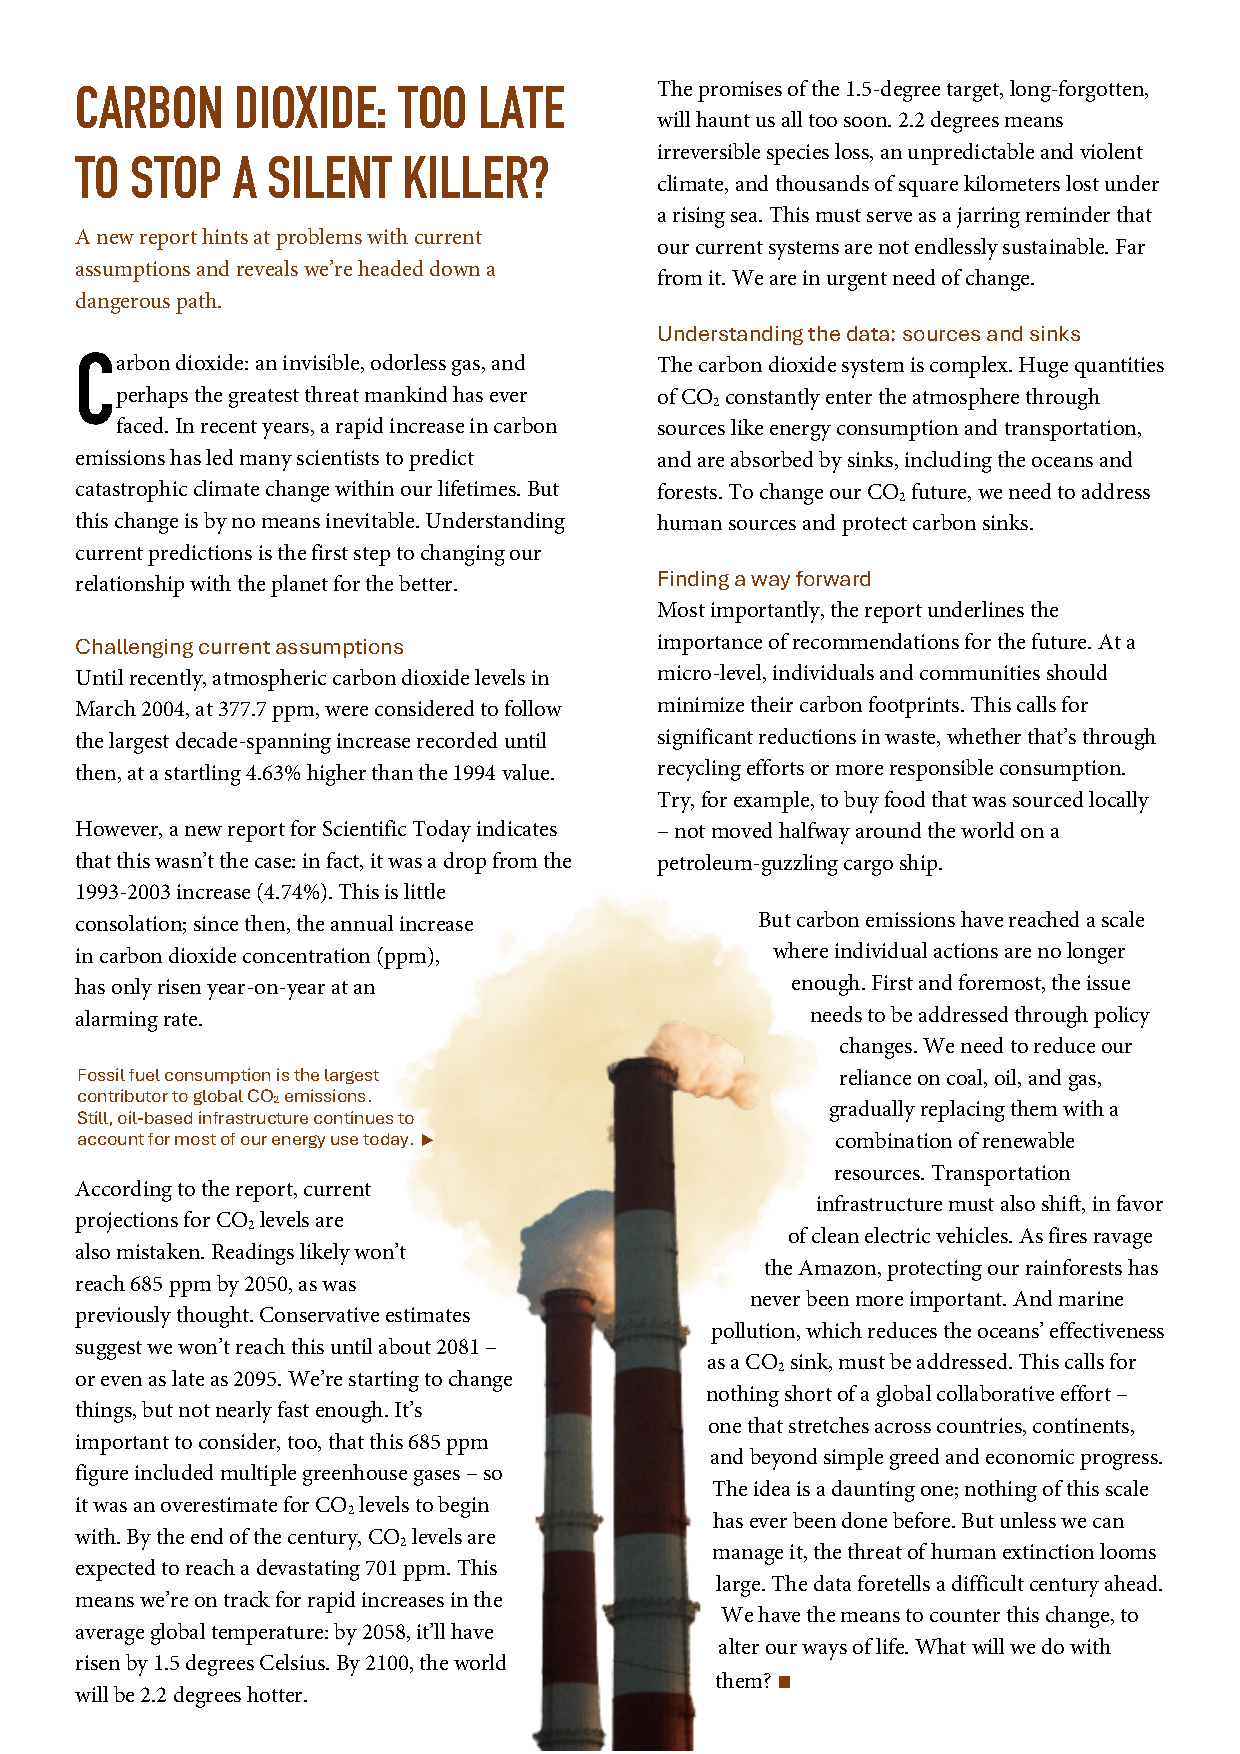
\includepdf[
        pages=-,
        addtotoc={1,section,1,New Report,a1}
    ]{article.pdf}


    \section{Introduction}

    \subsection{Background}
    The most significant greenhouse gas on Earth is carbon dioxide, which both absorbs and radiates heat. In contrast to oxygen and nitrogen, which together make up the majority of our atmosphere, greenhouse gases absorb heat emitted from the Earth's surface and re-emit it in all directions, including back toward the planet's surface. The natural greenhouse effect that keeps the Earth's atmosphere above freezing would be insufficient without carbon dioxide. People are accelerating the natural greenhouse effect and raising the earth's temperature by releasing more carbon dioxide into the atmosphere. The NOAA Global Monitoring Lab found that in 2021, carbon dioxide accounted for nearly two thirds of the total heating influence of all greenhouse gases created by humans.

    Prior to the Industrial Revolution, carbon dioxide in the atmosphere was consistently around 280 parts per million (ppm).
    The concentration of CO\textsubscript{2} in the atmosphere reached 377.7 ppm in March 2004, resulting in the largest 10-year average increase up to that time.
    According to scientists from National Oceanographic and Atmospheric Administration (NOAA) and Scripps Institution of Oceanography (SIO) the monthly mean CO\textsubscript{2} concentration level peaked at 421 ppm in May 2022.
    An Organisation for Economic Co-Operations and Development (OECD) report predicts a CO\textsubscript{2} level of 685 ppm by 2050.

    \subsection{Problem Analysis}
    \noindent\textbf{Problem 1: CO\textsubscript{2} level Forecasting}

    \begin{adjustwidth}{1cm}{}

        \noindent Modelling.

        \vspace{-6pt}
        \noindent Prodice models that reflect existing CO\textsubscript{2} data and extrapolates to reasonable predictions.

        \begin{adjustwidth}{1cm}{}
            \noindent Choose suitable mathematical models and fit each one to existing data.

            \noindent Evaluate each model\ldots~
            Use different evaluation approaches including statistical accuracy, contextual reasoning, comparison with external predictions, etc.

            \noindent Generate a conclusive model based on results obtained\ldots~
            Either pick the ``best'' model, or create new model based on multiple sub-parts.
        \end{adjustwidth}

        \noindent Verify External Claims.

        \begin{adjustwidth}{1cm}{}
            \noindent Whether CO\textsubscript{2} levels in 2004 had a ``larger increase than observed over any previous 10-year period''.

            \begin{adjustwidth}{1cm}{}
                \noindent Determine how exactly the comparison is done with ``any previous 10-year period''\ldots~
                Find supporting evidence from existing literature or make the best interpretation.
            \end{adjustwidth}

            \noindent Whether CO\textsubscript{2} levels will reach 685ppm by 2050.

            \begin{adjustwidth}{1cm}{}
                \noindent Testify this statement against all models.
            \end{adjustwidth}

        \end{adjustwidth}

        \noindent Draw Conclusions.

        \vspace{-6pt}
        \noindent Real-world implications based on predictions and results.

    \end{adjustwidth}


    \noindent\textbf{Problem 2: Temperature vs CO\textsubscript{2}}

    \begin{adjustwidth}{1cm}{}

        \noindent Modelling.

        \vspace{-6pt}
        \noindent Produce models that reflect existing temperature data and extrapolates to reasonable predictions.

        \begin{adjustwidth}{1cm}{}
            \noindent Direct relationship between CO\textsubscript{2} and temperature.

            \noindent Temperature as a time series, and compare with CO\textsubscript{2} models from Problem 1.
        \end{adjustwidth}

        \noindent Predictions.

        \vspace{-6pt}
        \noindent Predict points in time where global temperature will have an average increase of 1.25\textdegree C, 1.5\textdegree C, and 2\textdegree C compared to the base period of 1951--1980.

        \noindent Evaluation.

        \vspace{-6pt}
        \noindent Longevity \& Confidence; discuss the distance into the future that the model can still predict with reasonable accuracy.


    \end{adjustwidth}

    \bigskip

    \noindent Our thought process and plan is presented here below as a flowchart:
    \begin{center}
        \makebox[\textwidth]{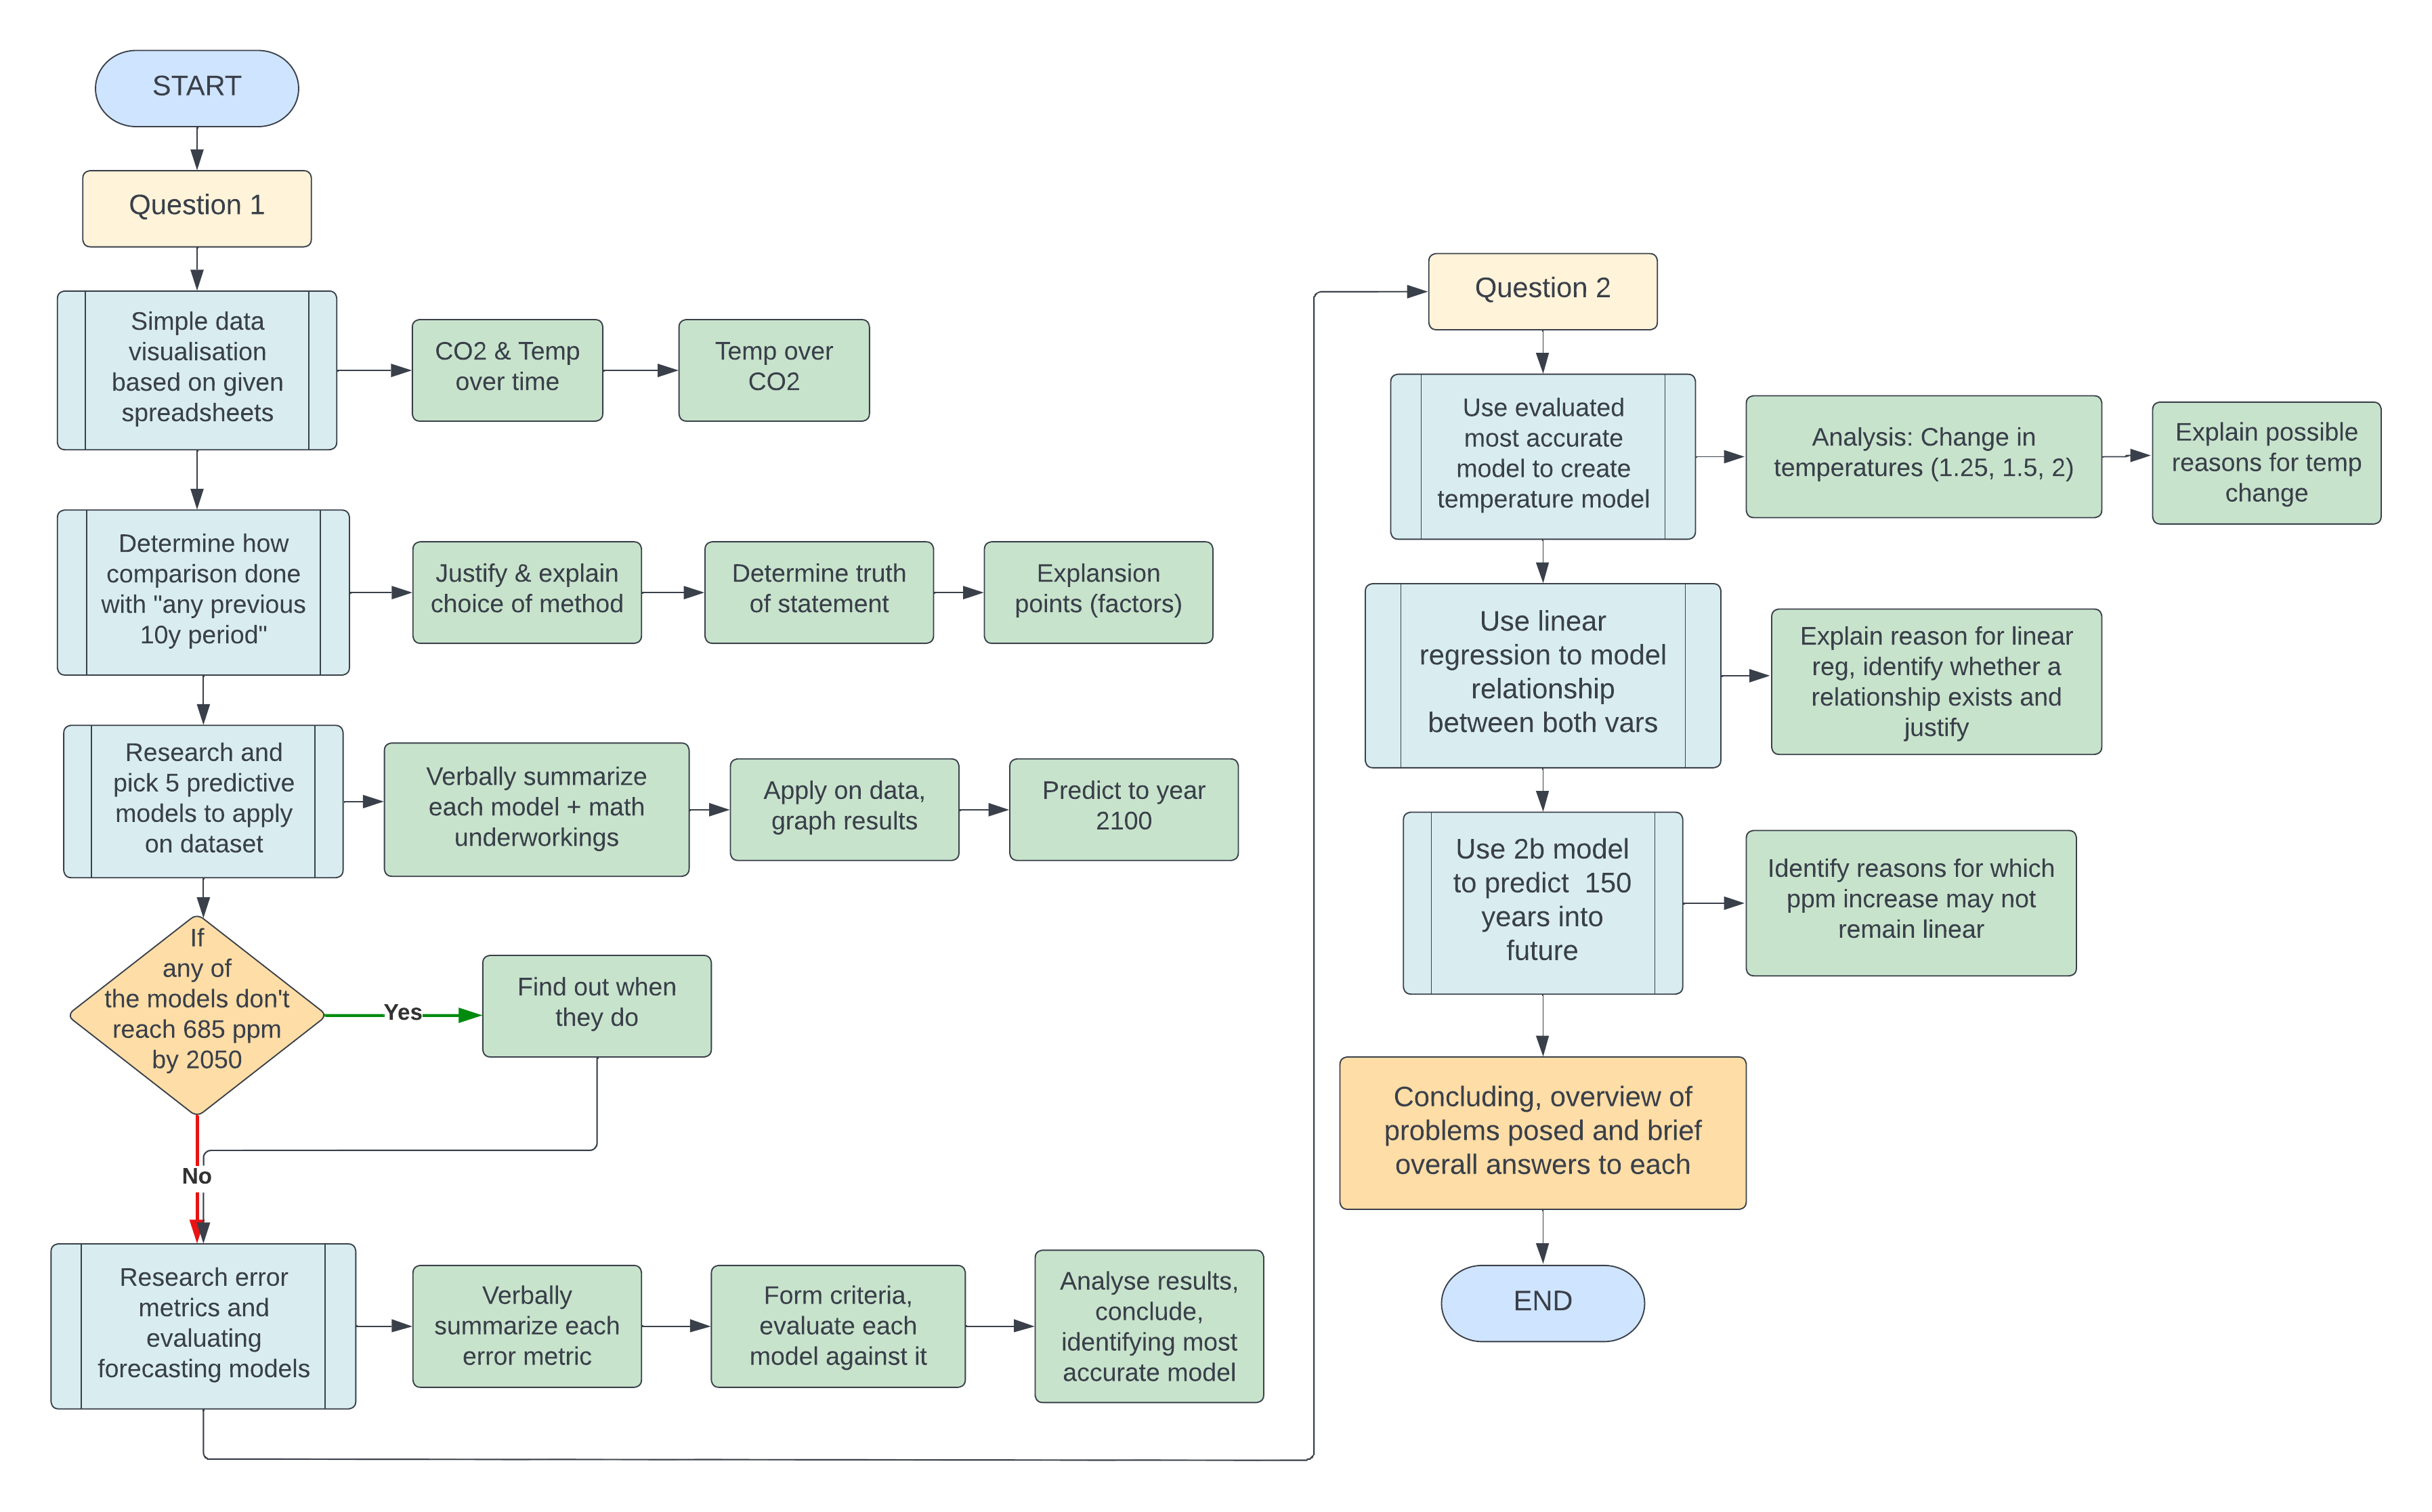
\includegraphics[width=\textwidth]{plan}}
    \end{center}

    \subsection{Keyword Definitions}
    \noindent\textbf{CO\textsubscript{2} Level/Content}: Global average concentration of CO\textsubscript{2} in the atmosphere, in parts-per-million (ppm).

    \noindent\textbf{Relative Temperature}: Global average temperature, relative to the baseline average temperature from 1951 to 1980, in degrees Celsius.

    \noindent\textbf{Error and Relationship Metric Abbreviations}: See Table~\ref{tab:err_abb}.

    \begin{table}[H]
        \centering
        \begin{tabular}{ll}
            \toprule
            Abb.                 & Full Name                                    \\
            \midrule
            MSE                  & Mean Squared-Error                           \\
            RMSE                 & Square Root of MSE                           \\
            MAE                  & Mean Absolute Error                          \\
            PCC                  & Pearson's Correlation Coefficient            \\
            R\textsuperscript{2} & Coefficient of Determination, or PCC Squared \\
            CVAR                 & Covariance                                   \\
            \bottomrule
        \end{tabular}
        \vspace{8pt}
        \caption{Abbreviations of Important Metrics}
        \label{tab:err_abb}
    \end{table}

    \subsection{Assumptions and Justifications}
    \noindent\textbf{Assumption 1}: CO\textsubscript{2}, as a greenhouse gas, has a true case-and-effect relationship with temperature.

    \vspace{-6pt}
    \noindent\textbf{Justification}: Most existing literature and evidence suggest that CO\textsubscript{2} is a greenhouse gas, and that greenhouse gases traps heat and leads to increases in temperature on a global scale. This fact is taken for granted to make more confident predictions that relate temperature to CO\textsubscript{2} levels.

    \noindent\textbf{Assumption 2}: Both datasets provided for CO\textsubscript{2} emissions and temperatures are reliable and accurate.

    \vspace{-6pt}
    \noindent\textbf{Justification}: Accurate predictions are always based on accurate data. Since official data is given along the problem, they will be taken and treated assuming the absence of mistakes and errors.

    \subsection{General Variables}
    See table~\ref{tab:my_label}:

    \begin{table}[h!]
        \centering
        \begin{tabular}{cc}
            \toprule
            Variable   & Definition                                                    \\
            \midrule
            $C_i$      & CO\textsubscript{2} level at year $i$, in~\si{ppm}            \\
            $T_i$      & Temperature at year $i$, in~\si{\degree C}                    \\
            $C^{-1}_i$ & Year where (predicted) CO\textsubscript{2} is at $i$~\si{ppm} \\
            $T^{-1}_i$ & Year where (predicted) Temperature is at $i$~\si{\degree C}   \\
            \bottomrule
        \end{tabular}
        \vspace{8pt}
        \caption{General Variables}
        \label{tab:my_label}
    \end{table}


    \section{The Generic Modelling Procedure}
    In this section, the generic procedure to produce specific models for a given task is stated and explained. All relevant information; such as metrics, concepts, and terms; are explained and directly referred to later. This section helps avoid bloat in the paper by isolating generic baseline information to prevent repetition and confusion.

    \subsection*{Modelling, Conceptually}

    ``A mathematical model is a description of a \textit{system} using mathematical concepts and language.'' (wikipedia reference) A completed math model should describe/simulate it\textquotesingle s target system to the best of its ability. All models behave like a (complex) function~\eqref{eq:model_func} - it produces outputs when given inputs. For this problem, the \textit{system}s to be modelled are atmospheric CO\textsubscript{2} and global warming.
%
    \begin{equation}
        y = f(x)
        \label{eq:model_func}
    \end{equation}
%
    \noindent where $y$ is the output, $x$ is the input, and $f$ is the model itself.

    \subsection*{Time Series}

    Inputs and outputs differ depending on the type of the model, but one type relevant to this paper is are time-series\textquotesingle . In a time-series model, the input is a timeframe, and the output describes the state of a system it is modelling; conceptually, a time-series models the evolution of a possibly boundless dynamic system over time~\eqref{eq:model_ts}. This will be useful later to, for example, model the change of CO\textsubscript{2} levels over time. Time-series\textquotesingle~belong to the family of relationship models, which produces outputs based on an input variable, effectively translation values between two variables. This will be useful later to model the relationship between CO\textsubscript{2} levels and temperature change.
%
    \begin{equation}
        \begin{aligned}
            t & \rightarrow y \\
            \Delta t & \rightarrow \Delta y + y_0
        \end{aligned}
        \label{eq:model_ts}
    \end{equation}
%
    \noindent where $y$ is the output, $t$ is the time or input, and $y_0$ is the initial state (when modelling relative evolution over time).

    \subsection*{Quantitative Data}

    Because math models are strictly quantitative, a pre-defined procedure must exist to translate between real-world parameters and numeric values. For most systems, this can be done using existing scientific measurements and units. Otherwise, custom metrics have to be defined. With the given problem, there are simple metrics for both CO\textsubscript{2} levels in the atmosphere and global warming, concentration in parts-per-million and temperature in degrees Celsius, respectively. In terms of time, years are already represented numerically.

    Once the system can be represented quantitatively and a quantitative output can be interpreted as a state of the system, a math model can be constructed. There are many different approaches to construct a model from numerical representations of a system, but this paper focuses on ``fitting'' ``generic models'' to true/historical numeric data.

    \subsection*{Function Regression}

    In short, a ``generic model'' is a mathematical function parameterized by a variable amount of constants within its definition~\eqref{eq:model_g}. The function exhibits specific characteristics regardless of the values of its parameters. The end goal of modelling is to adjust these parameters such that the function can produce the most accurate output (compared to the real system) for each given input. In the case of modelling CO\textsubscript{2} levels as a time-series, the model function should produce ppm values for a given year.
%
    \begin{equation}
        \begin{aligned}
            \bm{\beta} &= [p_1, p_2, p_3, p_4, \dots] \\
            f(x) &= g(x, \bm{\beta}) \\
            y &= f(x)
        \end{aligned}
        \label{eq:model_g}
    \end{equation}
%
    \noindent where $g$ is the generic model, and $f$ is a constructed model by finding specific values for each of the parameters $p_i$. $\bm{\beta}$ is simply a vector that encapsulates all of the parameters.

    \subsection*{Error Metrics}

    ``Fitting'' a model, also known as ``optimization'', is a systematic approach to find parameters that ``best'' models the given system. Usually, an error function is defined to quantitatively gauge how accurate or good the model is by calculating a metric based on the difference between the actual output and expected output for a given input~\eqref{eq:model_diff}. The optimization process tries to produce the ``best'' model by minimizing the error function across all available data values. For example,~\eqref{eq:model_sqd} is a square-error function that gives the sum of square-errors for all data points.
%
    \begin{equation}
        E(y) \approx y - \hat y
        \label{eq:model_diff}
    \end{equation}

    \begin{equation}
        E_{sum} = \sum_{i=1}^{n} (f(x_i) - \hat y_i)^2
        \label{eq:model_sqd}
    \end{equation}

    \subsection*{Optimization}

    The optimization process aims to minimize the (sum of the) error function.
    A generic approach is to take partial derivatives of the summed error with respect to every parameter in the model. This allows the minimum to be calculated by equating the differential functions to 0.
    Generally, the partial derivative of error $E$ with respect to parameter $\beta_j$ is:
%
    \begin{equation}
        \begin{aligned}
            \frac{\partial E}{\partial \beta_j} &= 2 \sum_i e_i \frac{\partial e_i}{\partial \beta_j} \\
            \frac{\partial E}{\partial \beta_j} &= -2\sum_i e_i\frac{\partial f(x_i,\boldsymbol \beta)}{\partial \beta_j}
        \end{aligned}
    \end{equation}
%
    \noindent where $e$ is the error, and $j = 1, \ldots, m$ for $m$ parameters in $\beta$.



    \section{CO\textsubscript{2} - Modelling}
    This section includes a walk through of all mathematical models used to model the CO\textsubscript{2} levels as a time series and how they specifically apply to the given data.

    \subsection{Pre-Analysis}
    Firstly, this problem takes the form of a single-variable time series; CO\textsubscript{2} levels evolve as time passes, and we are trying to model the relationship between time and CO\textsubscript{2}.
    Based on simple logic and scientific reasoning, there is no cause-and-effect relationship between time and carbon dioxide levels, so the models will assume a relationship that is purely a statistical correlation.

    The given CO\textsubscript{2} data is graphed to visualize the rough correlation and trend present in the data (Figure~\ref{fig:co2}). It is very apparent that there is a strong correlation with minimal variance between time and carbon dioxide levels. The shape of the curve seems exponential. These ideas will be help guide future mathematical modelling.
    Auto-correlation is calculated to identify any seasonality within the data (Figure~\ref{fig:co2_acf}). However, it is apparent that there is no clear seasonality within the data, as shown by the lack of an oscillating correlation. This is expected since the data comes in annual resolutions; yearly seasonality could be expected due to seasonal effects, but would only be observed with monthly data.

    \begin{figure}[h]
        \centering
        \begin{minipage}{.5\textwidth}
            \centering
            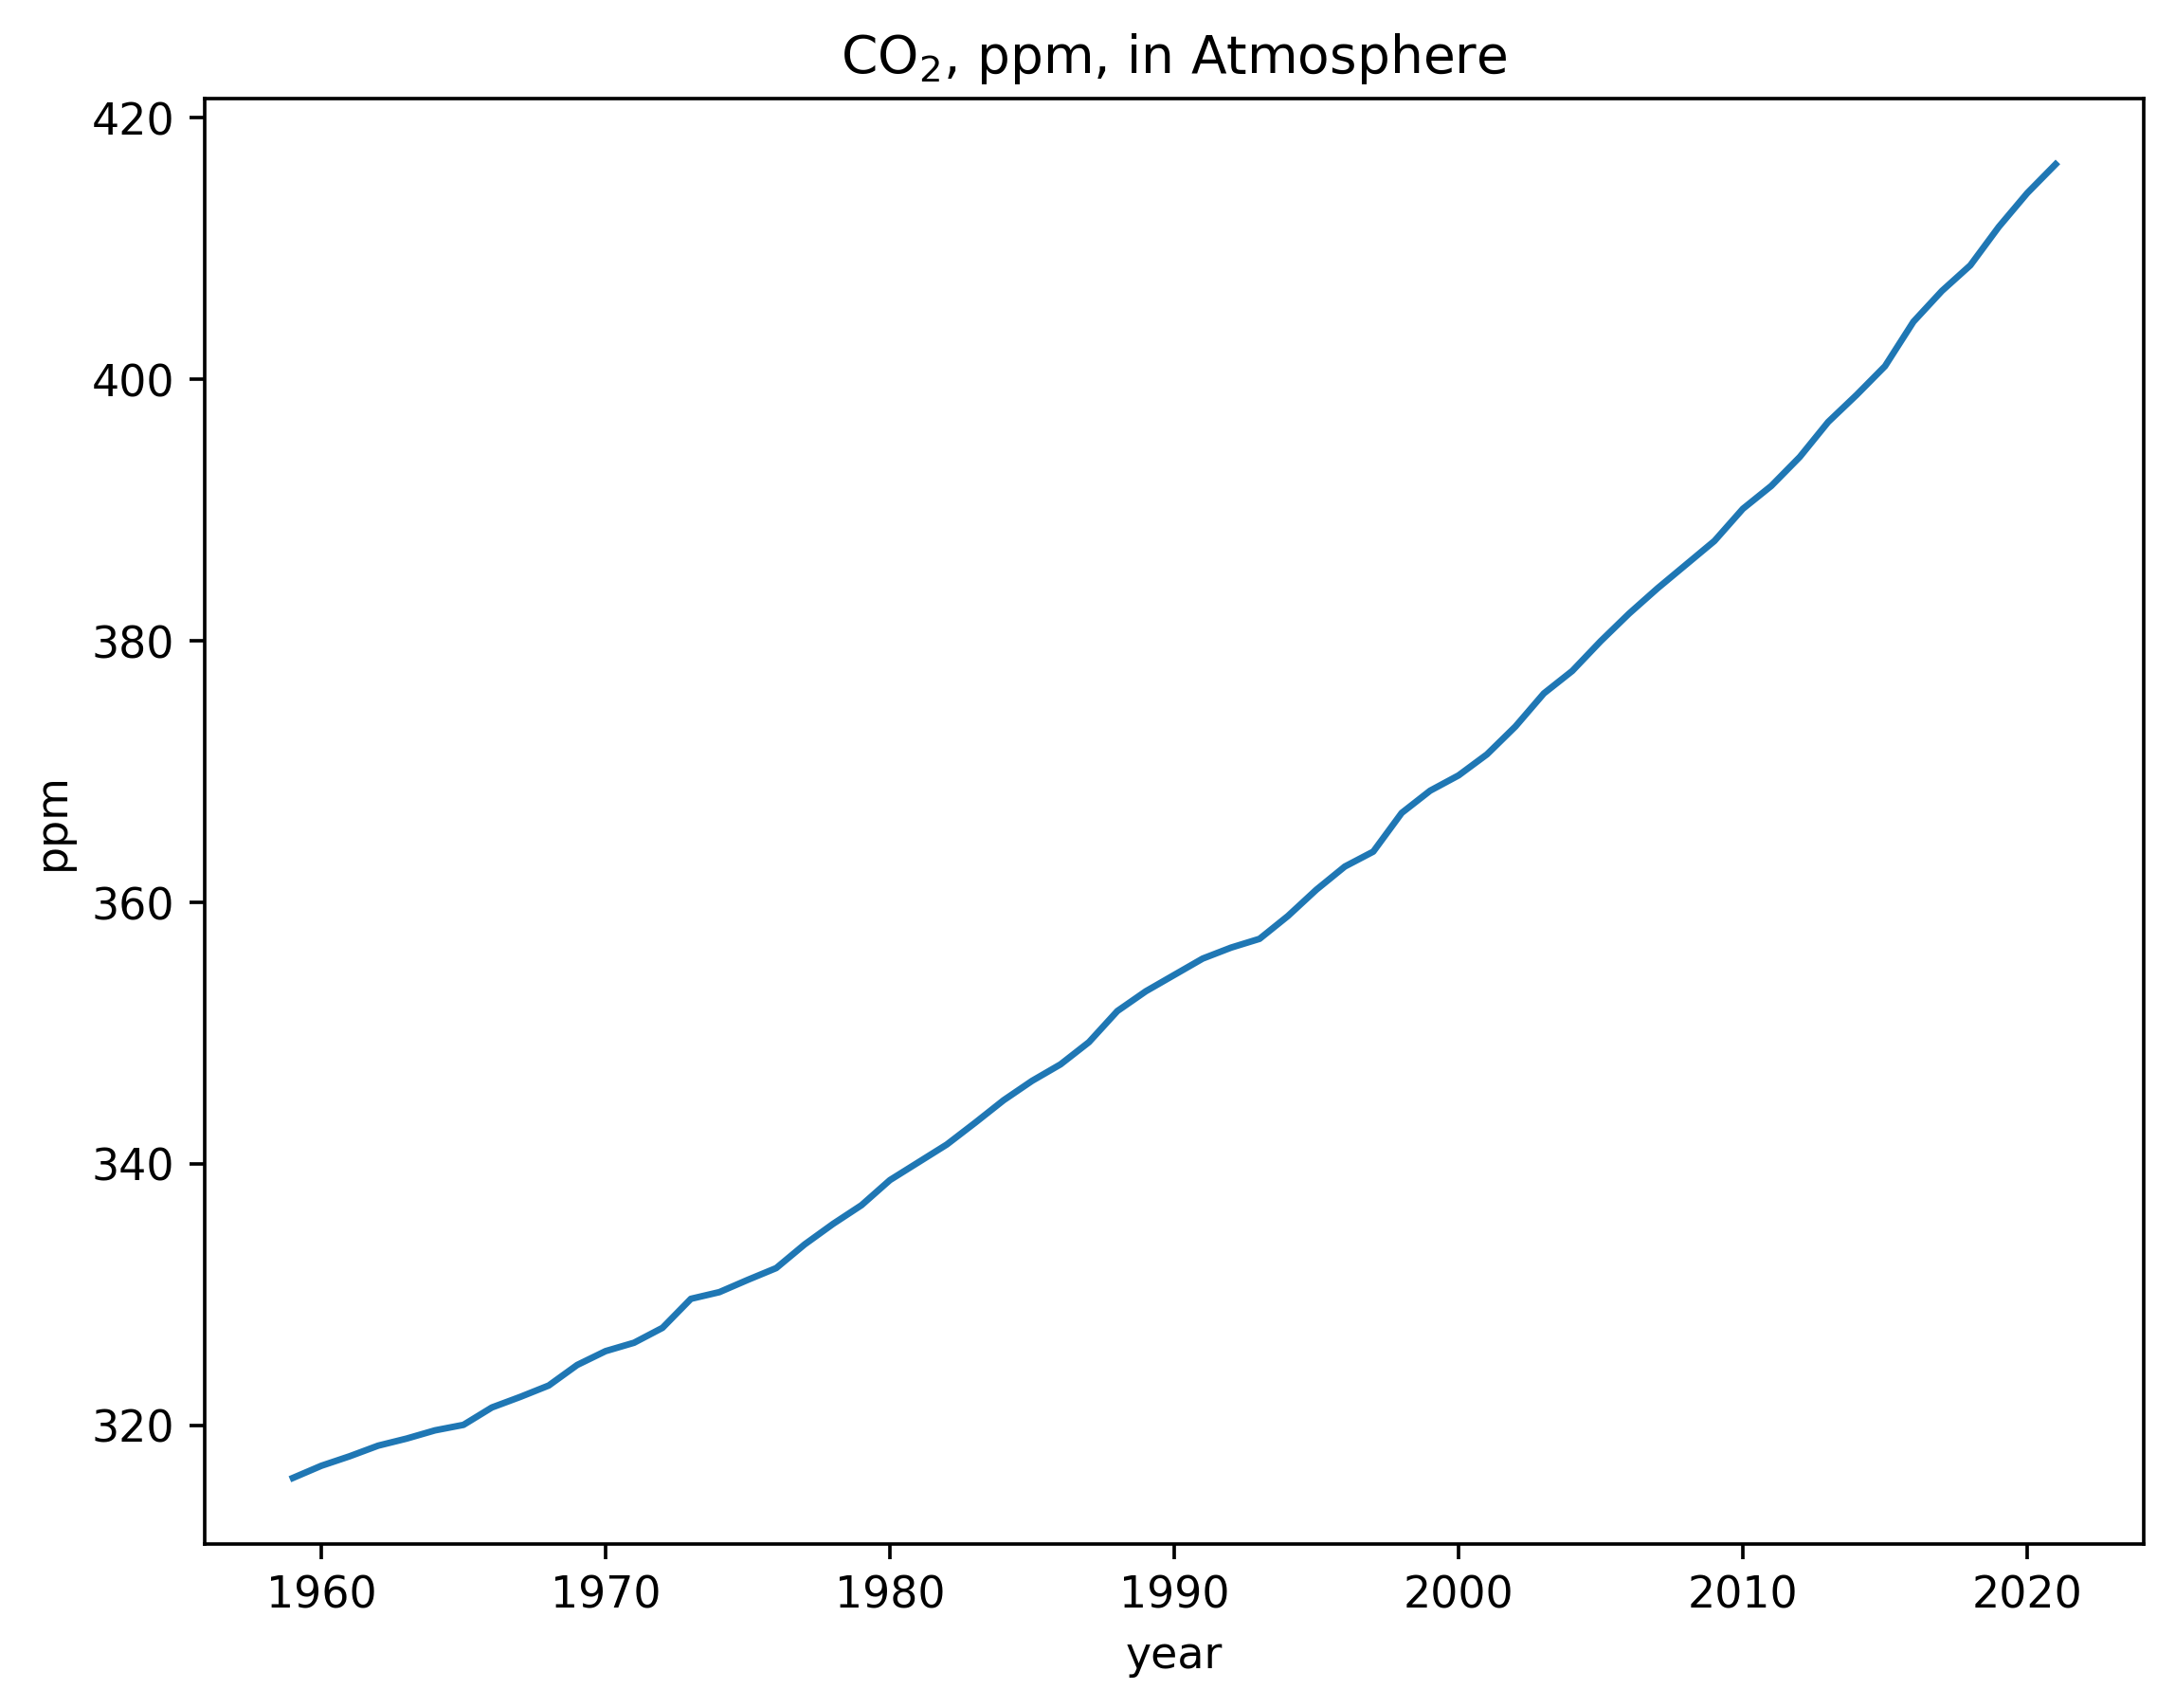
\includegraphics[width=\textwidth]{co2}%
            \caption{Graph of given CO\textsubscript{2} data}
            \label{fig:co2}
        \end{minipage}%
        \begin{minipage}{.5\textwidth}
            \centering
            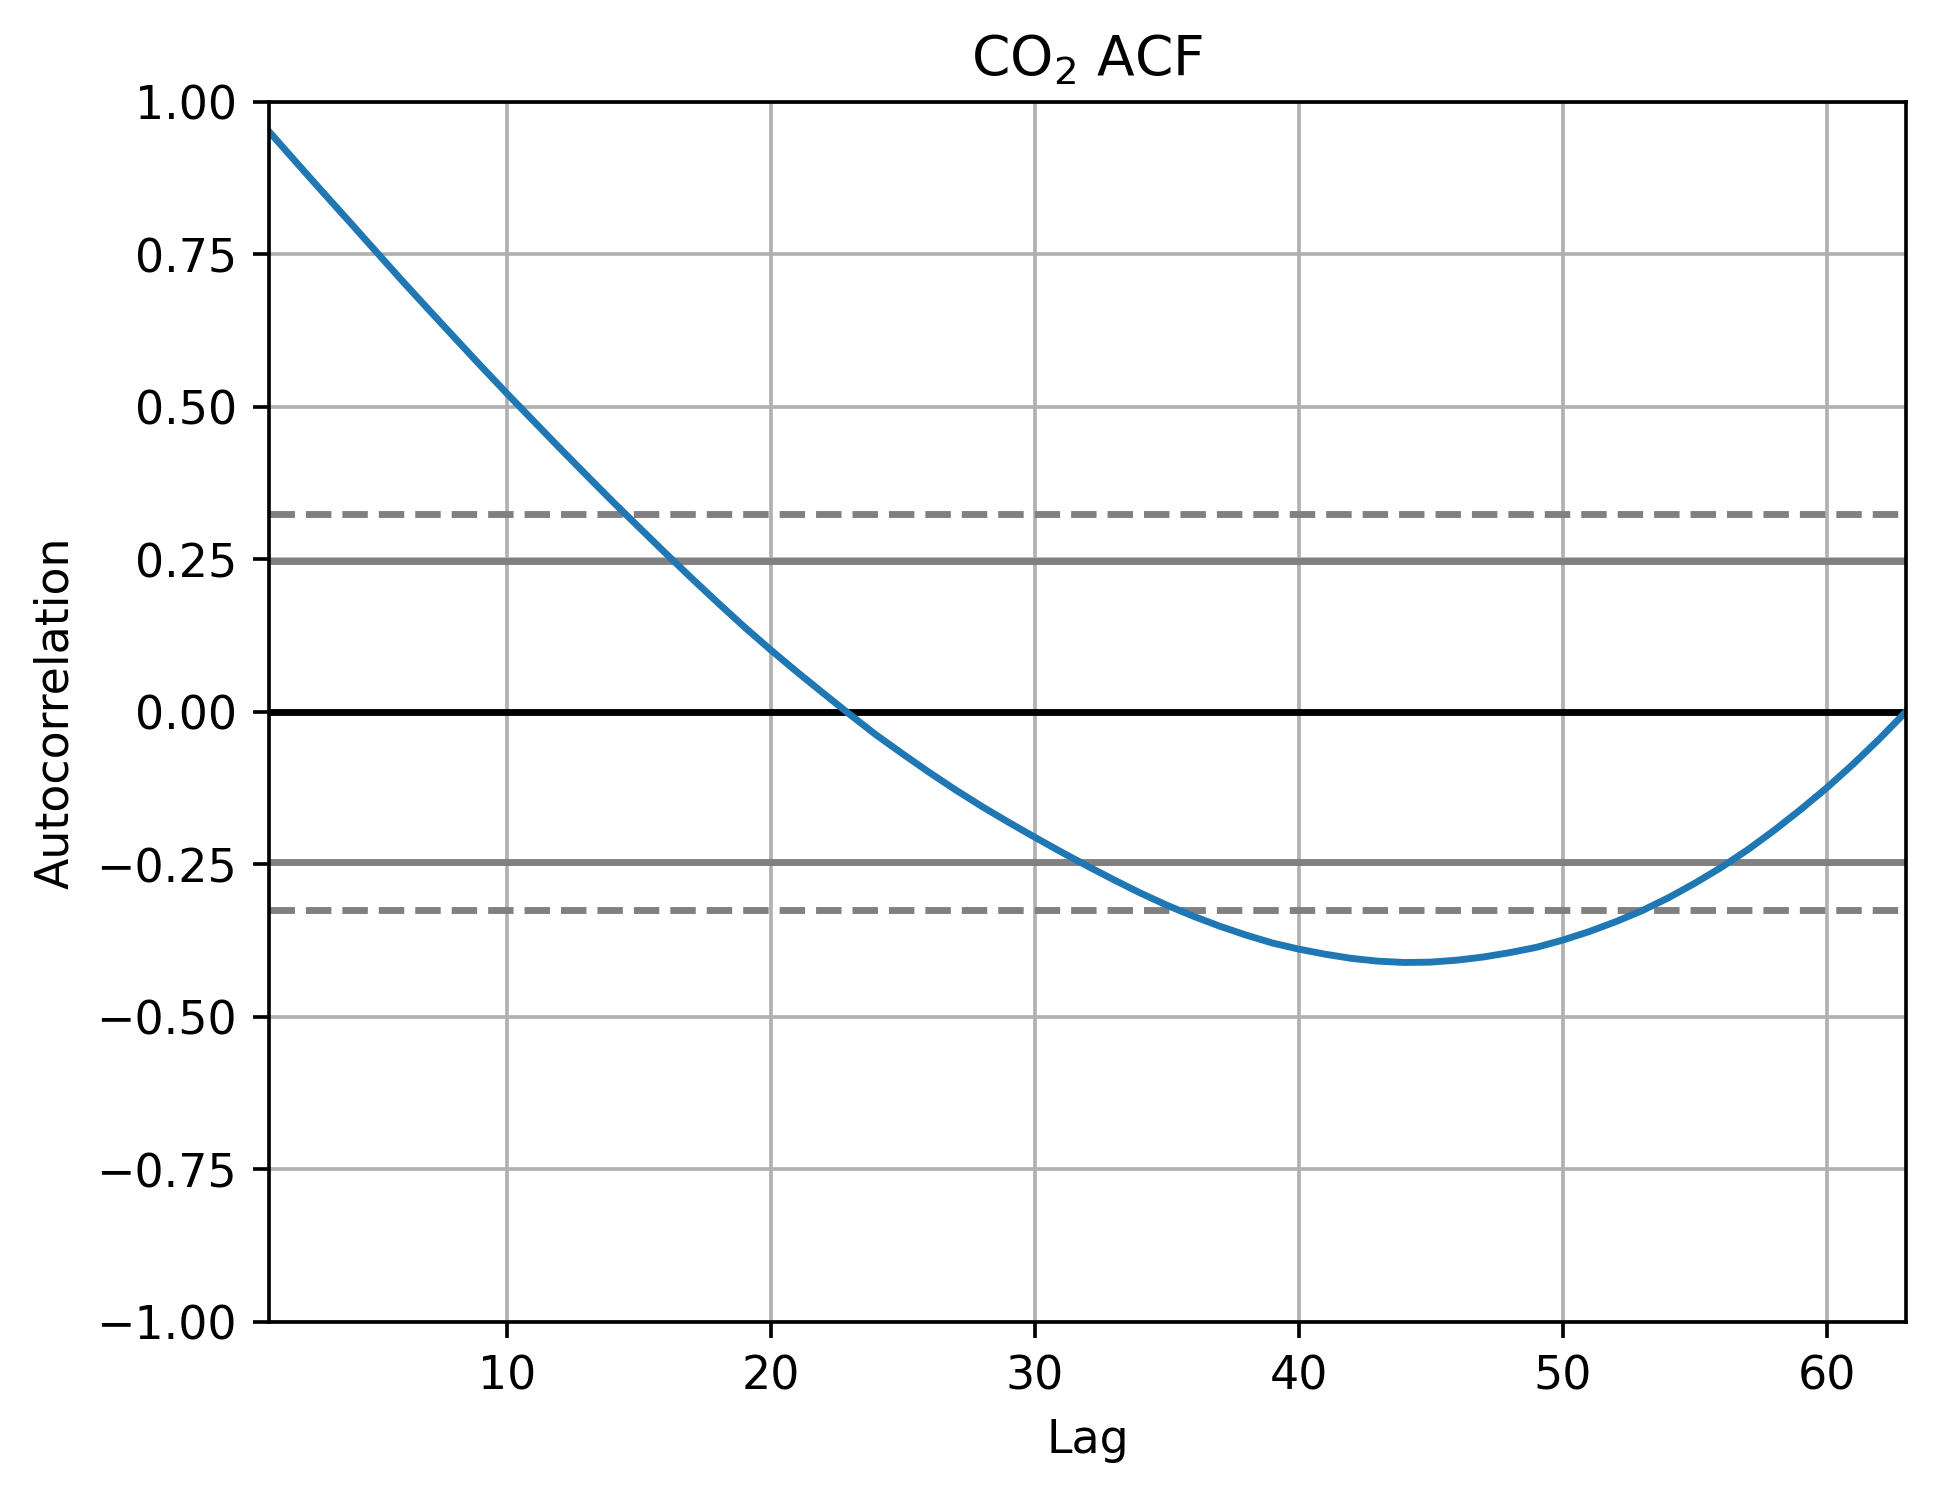
\includegraphics[width=\textwidth]{co2_acf}%
            \caption{CO\textsubscript{2} Auto-correlation}
            \label{fig:co2_acf}
        \end{minipage}
    \end{figure}

    \subsection{Linear}
    A linear regression is performed first due to its simplicity and ability to help pick more complex models.

    Linear regression is an approach used to model a linear relationship between an independent variable $x$ and a dependent variable $y$ by finding the slope of the trend and initial value ($y$ when $x$ is 0).
    It is used to represent existing data and predict future values; linear models are used both for interpolation and extrapolation. In this case, the model will be fit to existing data and used to predict future CO\textsubscript{2} levels.
    A linear growth function takes the general form of~\eqref{eq:lr}:
%
    \begin{equation}
        f(x) = \alpha x + \beta
        \label{eq:lr}
    \end{equation}
%
    \noindent where $\alpha$ is the coefficient, or growth rate; and $\beta$ is the y-intercept, or initial value.
    The values of $\alpha$ and $\beta$ are ``optimized'' using an algorithm to model a given dataset with the minimum ``error''.

    One of the most common and simplest methods used to calculate the coefficient and intercept of the regression line is the Ordinary Least Square (OLS) \textit{optimization} method.
    In short, OLS minimizes the Square-Error for each point against a given linear function by adjusting the function\textquotesingle s parameters, which in the end produces optimal parameters for a equation in the form of a linear line of best fit.

    The Square-\textit{Error} function, which is what OLS \textit{optimizes}, is simply a summation of the squares of the difference between actual values and predicted values, over all data points~\eqref{eq:ls}:

    \begin{equation}
        E = \sum{(y - \hat{y})^2}
        \label{eq:ls}
    \end{equation}

    Because the predicted values $\hat{y}$ for a linear model is modelled as $\alpha x + \beta$, the Square-Error function for a linear model can be more specific~\eqref{eq:ls_lr}:

    \begin{equation}
        E = \sum{(y - (\alpha x + \beta))^2}
        \label{eq:ls_lr}
    \end{equation}

    OLS calculates the values of $\alpha$ and $\beta$ which minimize $S$ in the summation above.
    Unlike the generic differential method described above, OLS is specialized for linear functions and can calculate the optimal parameters in one stop, using summation ratios.
    The coefficient $\alpha$, or the linear trend of the dataset can be calculated with~\eqref{eq:lr_coef}:

    \begin{equation}
        \alpha = \frac{n \sum x_i y_i - \sum x_i \sum y_i }{n \sum x^2_i - (\sum x_i)^2}
        \label{eq:lr_coef}
    \end{equation}

    \noindent where $n$ is the number of data points.

    After calculating the slope of the trend, the intercept $\beta$, is calculated by~\eqref{eq:lr_intc}:
%
    \begin{equation}
        \beta = \bar y - \alpha \bar x
        \label{eq:lr_intc}
    \end{equation}

    OLS was applied to the given data set to obtain the coefficient $\alpha$ and the y-intercept $\beta$ - $1.6140361$ and $-2854.59326421$, respectively - which corresponds to the following linear equation:
%
    \begin{equation}
        \hat C_i = 1.6140361 i - 2854.59326421
        \label{eq:co2_lr}
    \end{equation}
%
    \noindent where $i$ is the year.

    The inverse of the function is derived by solving for $i$ in terms of $C$:

    \begin{equation}
        \hat C^{-1}_i = \frac{C + 2854.59326421}{1.6140361}
        \label{eq:co2_lr_inv}
    \end{equation}

    $C$ was then set to 685 to find the year at which CO\textsubscript{2} emissions would reach 685ppm; it was found that it would reach this level at the year 2193.
    The regression line was then graphed and used to predict the next 30 years of CO\textsubscript{2} emissions; the actual data is also plotted for comparison (Figure~\ref{fig:co2_lr}).


    Linear regression is useful in relation to the problem as it is simple to interpret and portray, allowing the prediction of data to be accurate during interpolation.
    However, if the data to be predicted is outside of the range, such as predicting future CO\textsubscript{2} levels, extrapolation may be inaccurate due to a false assumption of the trend.
    Furthermore, if the variables plotted provide a non-linear relationship, a linear regression line may inaccurately represent and predict values, which is the case in the data provided.
    Statistical error of the linear regression model against existing data shows a good but not perfect accuracy (Table~\ref{tab:co2_lr_err}).

    \begin{table}[h]
        \begin{minipage}{0.7\linewidth}
            \centering
            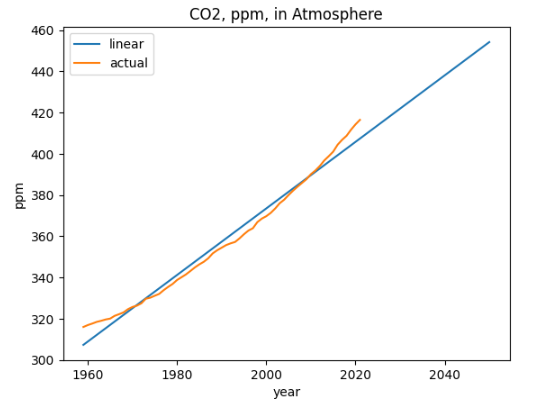
\includegraphics[width=\textwidth]{linear}%
            \captionof{figure}{Graph of given CO\textsubscript{2} data}
            \label{fig:co2_lr}
        \end{minipage}%
        \begin{minipage}{0.3\linewidth}
            \centering
            \begin{tabular}{ll}
                \toprule
                Metric               & Value  \\
                \midrule
                MSE                  & 15.376 \\
                RMSE                 & 3.9212 \\
                MAE                  & 3.1920 \\
                PCC                  & 0.9912 \\
                R\textsuperscript{2} & 0.9825 \\
                CVAR                 & 875.32 \\
                \bottomrule
            \end{tabular}
            \vspace{8pt}
            \caption{Linear Model Statistics}
            \label{tab:co2_lr_err}
        \end{minipage}
    \end{table}

    \subsection{Exponential}
    The second approach decided upon was exponential regression, which models the non-linear relationship between an independent variable $x$ and dependent variable $y$, where the rate of change of $y$ with respect to $x$ at a given point is proportional to the quantity itself.
    This choice was made based on visual indicators of the data given\textquotesingle s trend, where the line graph exhibited a possible exponential curve.
    Exponential growth functions take the general form of~\eqref{eq:exp}:
%
    \begin{equation}
        f(x) = \alpha^x
        \label{eq:exp}
    \end{equation}
%
    \noindent where $\alpha$ is the exponential growth factor.

    However, in order to fit such a model to arbitrary (non-normalized) values, two additional parameters have to be added to allow for displacement translations of the function on both axis. This gives:
%
    \begin{equation}
        f(x) = \beta (\alpha)^{x + a} + b
        \label{eq:exp2}
    \end{equation}
%
    \noindent where $a$ and $b$ allows for offsets in the x and y axis, respectively.

    An optimization can be made here - the equation can be rearranged to only have 3 parameters yet still be able to fit to any scale and offset of values:
%
    \begin{equation}
        f(x) = B^{b (x + a)} + c
        \label{eq:exp3}
    \end{equation}
%
    \noindent where $B$, the base, can be any positive constant, and the function is parameterized by $a$, $b$, and $c$.

    $a$ and $b$ performs a linear transformation on the input, while $c$ performs a translation on the output.
    The equation in this form expresses in the relationship in purely in terms of translations.
    This reduction in parameters allows for a higher efficiency when regressing the function to the dataset programmatically.
    In the actual regression, 2 was used for the value of $B$.

    Unlike linear regression, trying to fit an exponential function to a data set would theoretically require complex methods such as partial derivatives.
    However, a programmatic approach was taken, and the function was ``blindly'' regressed using gradient descent (Alg.~\ref{alg:grad}) from derivative estimates.
    The \verb|curve_fit()| optimizer from the Python SciPy library can optimize any non-linear function to a dataset blindly - without knowing the algebraic denotation of the function.
    It is able to optimize unknown functions by performing gradient estimates~\eqref{eq:grad} of the error function with respect to the parameters using the basic definition of the derivative (at a given point, $x$):
%
    \begin{equation}
        G = \frac{\Delta f(x)}{\Delta x} = \frac{f(x + \Delta x) - f(x)}{\Delta x}
        \label{eq:grad}
    \end{equation}
%
    \noindent where $G$ is the gradient of function $f$ at point $x$.
    $\Delta x$ is set to a very small value to increase accuracy for sensitive functions.

    After being able to calculate gradients of the error function at any point of the model function, a gradient descent algorithm~(\ref{alg:grad}) can be deployed to iteratively minimize the error function.
    The parameters are adjusted based the gradients of the error function:
%
    \begin{equation}
        \beta_j \longleftarrow \beta_j - \alpha \frac{E(x, \beta + \Delta \beta_j) - E(x, \beta)}{\Delta \beta_j}
    \end{equation}
%
    \noindent where parameter $\beta_j$ is adjusted based the error function $E$\textquotesingle s gradient - the parameter changes in to the opposite direction of the gradient in order to find the minimum of the error function.
    $\alpha$, the learning rate, is usually a very small value to prevent the parameters from changing too much at once.

    \begin{algorithm}
        \caption{Gradient Descent}
        \label{alg:grad}
        \begin{algorithmic}
            \Repeat
                \State $\epsilon \gets E(f(x, \mathbf{\beta}))$  \Comment{E is the error function}
                \State $\gamma \gets \frac{\Delta E(f(x, \mathbf{\beta}))}{\Delta \mathbf{\beta}}$  \Comment{calculate current gradient}
                \State $\mathbf{\beta} \gets \mathbf{\beta} - \alpha \gamma$  \Comment{$\alpha$ is the learning rate}
            \Until{$\epsilon$ \text{ is sufficiently small}}
            \State \Return $\mathbf{\beta}$ \text{ as the optimal parameters}
        \end{algorithmic}
    \end{algorithm}


    The SciPy curve fit optimizer was applied to the given data to obtain the following model:
%
    \begin{equation}
        \hat C_i = 2^{0.023381 (i - 1707.690634)} + 256.024002
        \label{eq:co2_exp}
    \end{equation}
%
    and $i$ was solved for $\hat C_i = 685$ to find that CO\textsubscript{2} levels will reach 685\si{ppm} in 2081.
    The exponential model was graphed alongside the actual values and the linear model for comparison in Figure~\ref{fig:co2_exp}.

    \begin{table}[h]
        \begin{minipage}{0.7\linewidth}
            \centering
            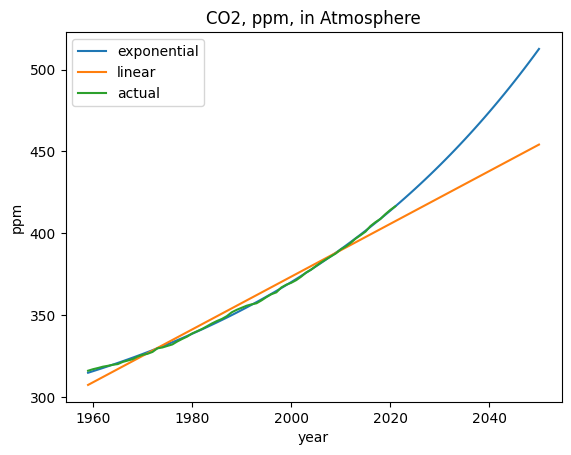
\includegraphics[width=\textwidth]{exponential}%
            \captionof{figure}{Graph of Exponential Regression}
            \label{fig:co2_exp}
        \end{minipage}%
        \begin{minipage}{0.3\linewidth}
            \centering
            \begin{tabular}{ll}
                \toprule
                Metric               & Value   \\
                \midrule
                MSE                  & 0.48061 \\
                RMSE                 & 0.69326 \\
                MAE                  & 0.56981 \\
                PCC                  & 0.99973 \\
                R\textsuperscript{2} & 0.99945 \\
                CVAR                 & 890.45  \\
                \bottomrule
            \end{tabular}
            \vspace{8pt}
            \caption{Exponential Model Statistics}
            \label{tab:co2_exp_err}
        \end{minipage}
    \end{table}

    Visually, the exponential function better aligns with the actual values; the predicted values also seem to fit with the general trend, and this is confirmed by extremely good error metrics, as show in Table~\ref{tab:co2_exp_err}.
    An advantage of exponential regression as a predictive model is that it provides high quality forecasts, which increase the accuracy of predicted values during interpolation.
    However, a key drawback is that a large data set is necessary to carry this method out, as a reasonable amount of continuity is needed to accurately predict future values, especially during extrapolation.

    \subsection{Sigmoid}
    The third predictive model selected shares similarities with the exponential model.
    While most sigmoid functions, when the domain is restricted, may behave very similar to an exponential function, the difference is that sigmoid functions also have an upper asymptote.
    The function has a S-shaped curve, comparable to two exponential functions, one with a negative exponent and one with a positive exponent, that are joined at the point of inflection.
    Sigmoid functions are commonly used to model growth variables with a natrual limit.
    The most common sigmoid function is the logistic function, which takes the general form of:
%
    \begin{equation}
        f(x) = \frac{L}{1 + e^{-k(x - x_0)}}
        \label{eq:logi}
    \end{equation}
%
    where
    $L$ is the curve\textquotesingle s maximum value,
    $k$ is the logistic growth rate, and
    $x_0$ is the x value of the sigmoid midpoint.

    The standard logistic function is, however, pretty limited; the minimum asymptote is fixed at zero and the shape of the curve is fixed other than the growth rate, which reflects the gradient at the midpoint.
    In order to fit to the CO\textsubscript{2} dataset, a more generalized and adjustable sigmoid function is used:
%
    \begin{equation}
        f(x) = \frac{x-x_{0}}{\left(s^{-z}+\frac{2\left|x-x_{0}\right|}{y_{max}-y_{min}}^{z}\right)^{\frac{1}{z}}}+\frac{y_{max}-y_{min}}{2}+y_{min}
    \end{equation}
%
    where
    $x_0$ is the x value of the sigmoid midpoint,
    $s$ is the growth rate or slope at the midpoint,
    $z$ governs the shape of the curve,
    $y_{max}$ is the maximum y value, and
    $y_{min}$ is the minimum y value.

    Removing parameters that allow linear transformations, the sigmoid function can be simplified to:
%
    \begin{equation}
        f(x) = \frac{x}{\left(s^{-z}+\frac{\left|x\right|}{L}^{z}\right)^{\frac{1}{z}}}
    \end{equation}
%
    and by removing the $z$ parameter, a basic algebraic sigmoid function remains:
%
    \begin{equation}
        f(x) = \frac{x}{s^{-1}+{\left|x\right|}/{L}}
    \end{equation}
%
    where
    $L$ is the curve\textquotesingle s maximum value (also the negative minimum; the function is centered at the origin) and
    $s$ is the growth rate or slope at the midpoint.

    Because the entire idea of a sigmoid function is that there is an upper limit, this limit has to be set before the other parameters defining the curve can be regressed against the dataset.
    If the limit left to the freedom of the optimizer, the output usually results in completely unreasonable limits, due to the fact that the optimizer will naively try to minimize the error function by adjusting any parameters necessary.
    This is demonstrated in Figure~\ref{fig:co2_logi_2400}, where the the limit was automatically regressed to beyond 2700\si{ppm}.
    The logistic function used was inflated so much that the sigmoid curve could only be seen on half-millennium time scales.

    To avoid this issue which causes sigmoid functions to regress into practically exponential functions in a short time frame, the limit set to values between 420 and 960\si{ppm} before the optimizer was applied. The range of sigmoid curves for different limits is shown in Figure~\ref{fig:co2_sigm_all}. As explored later, external sources predict a maximum CO\textsubscript{2} level within the near future (2070) to be around 565\si{ppm}, which is used as the limit of the final sigmoid model:
%
    \begin{equation}
        \hat C_i = \frac{x-2016.8}{\left(2.2796^{-1.4953}+\frac{2\left|x-2016.8\right|}{565-246.49}^{1.4953}\right)^{\frac{1}{1.4953}}}+\frac{565-246.49}{2}+246.49
        \label{eq:co2_sig}
    \end{equation}

    \begin{table}[h]
        \begin{minipage}{0.7\linewidth}
            \centering
            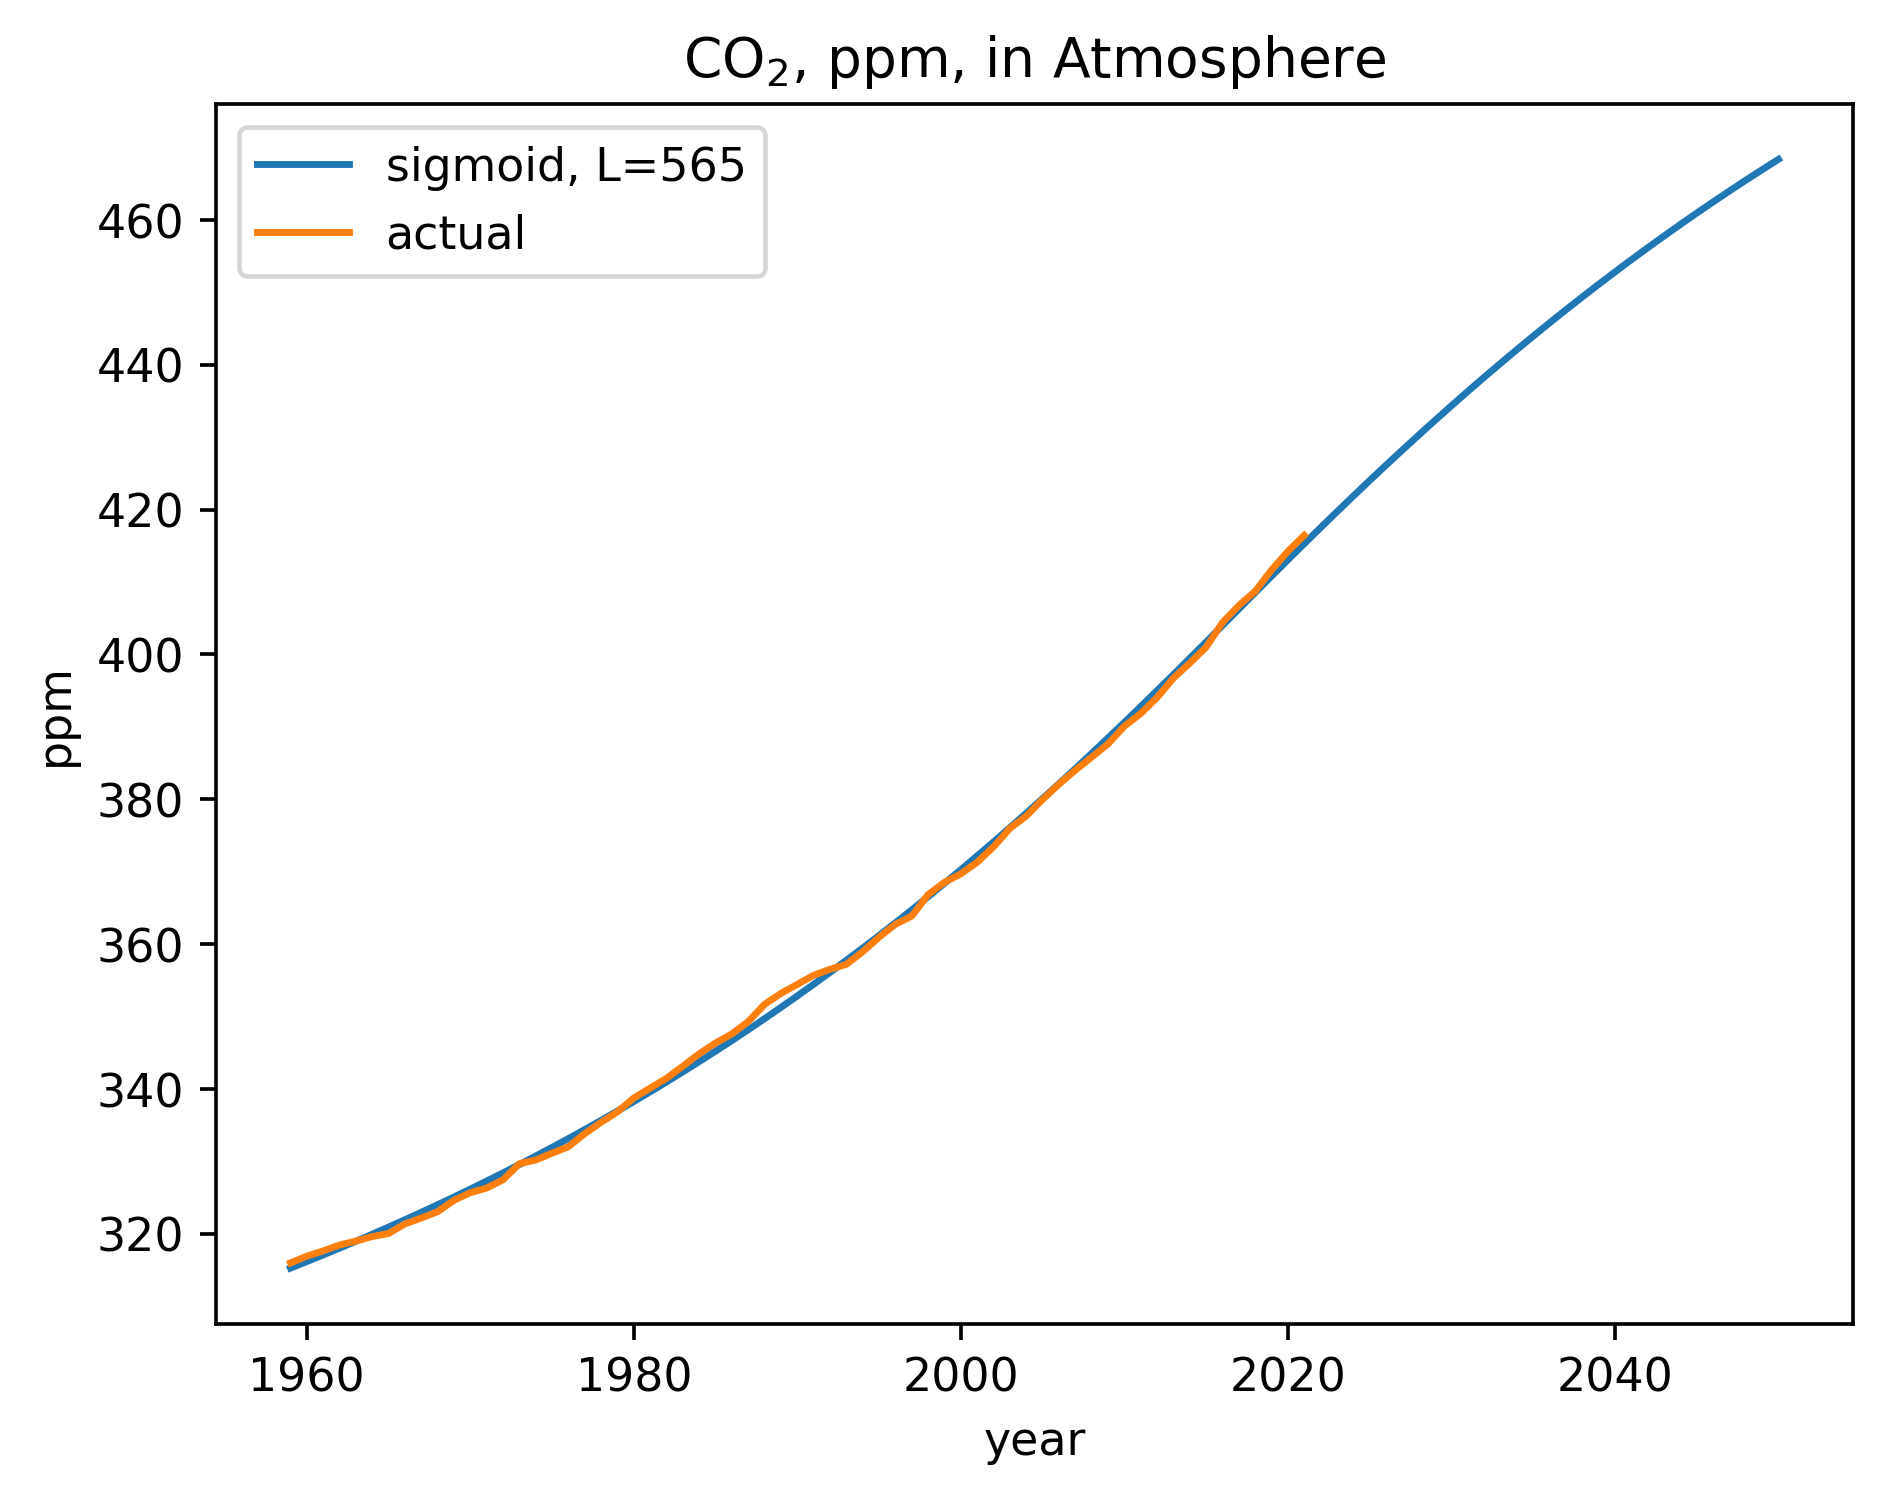
\includegraphics[width=\textwidth]{co2_sigm_565}%
            \captionof{figure}{Graph of Sigmoid Regression}
            \label{fig:co2_logi}
        \end{minipage}%
        \begin{minipage}{0.3\linewidth}
            \centering
            \begin{tabular}{ll}
                \toprule
                Metric               & Value   \\
                \midrule
                MSE                  & 0.61002 \\
                RMSE                 & 0.78104 \\
                MAE                  & 0.66351 \\
                PCC                  & 0.99965 \\
                R\textsuperscript{2} & 0.99930 \\
                CVAR                 & 889.87  \\
                \bottomrule
            \end{tabular}
            \vspace{8pt}
            \caption{Error Metrics for Sigmoid Regression}
            \label{tab:co2_logi_err}
        \end{minipage}
    \end{table}

    \begin{figure}[h]
        \begin{minipage}{0.5\linewidth}
            \centering
            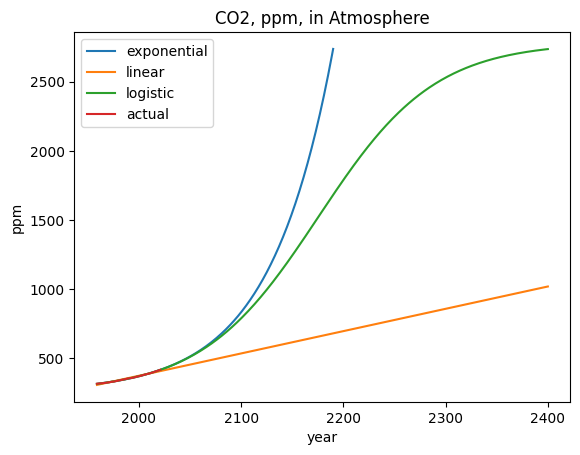
\includegraphics[width=\textwidth]{logistic_2400}%
            \captionof{figure}{Blown up Logistic Regression}
            \label{fig:co2_logi_2400}
        \end{minipage}%
        \begin{minipage}{0.5\linewidth}
            \centering
            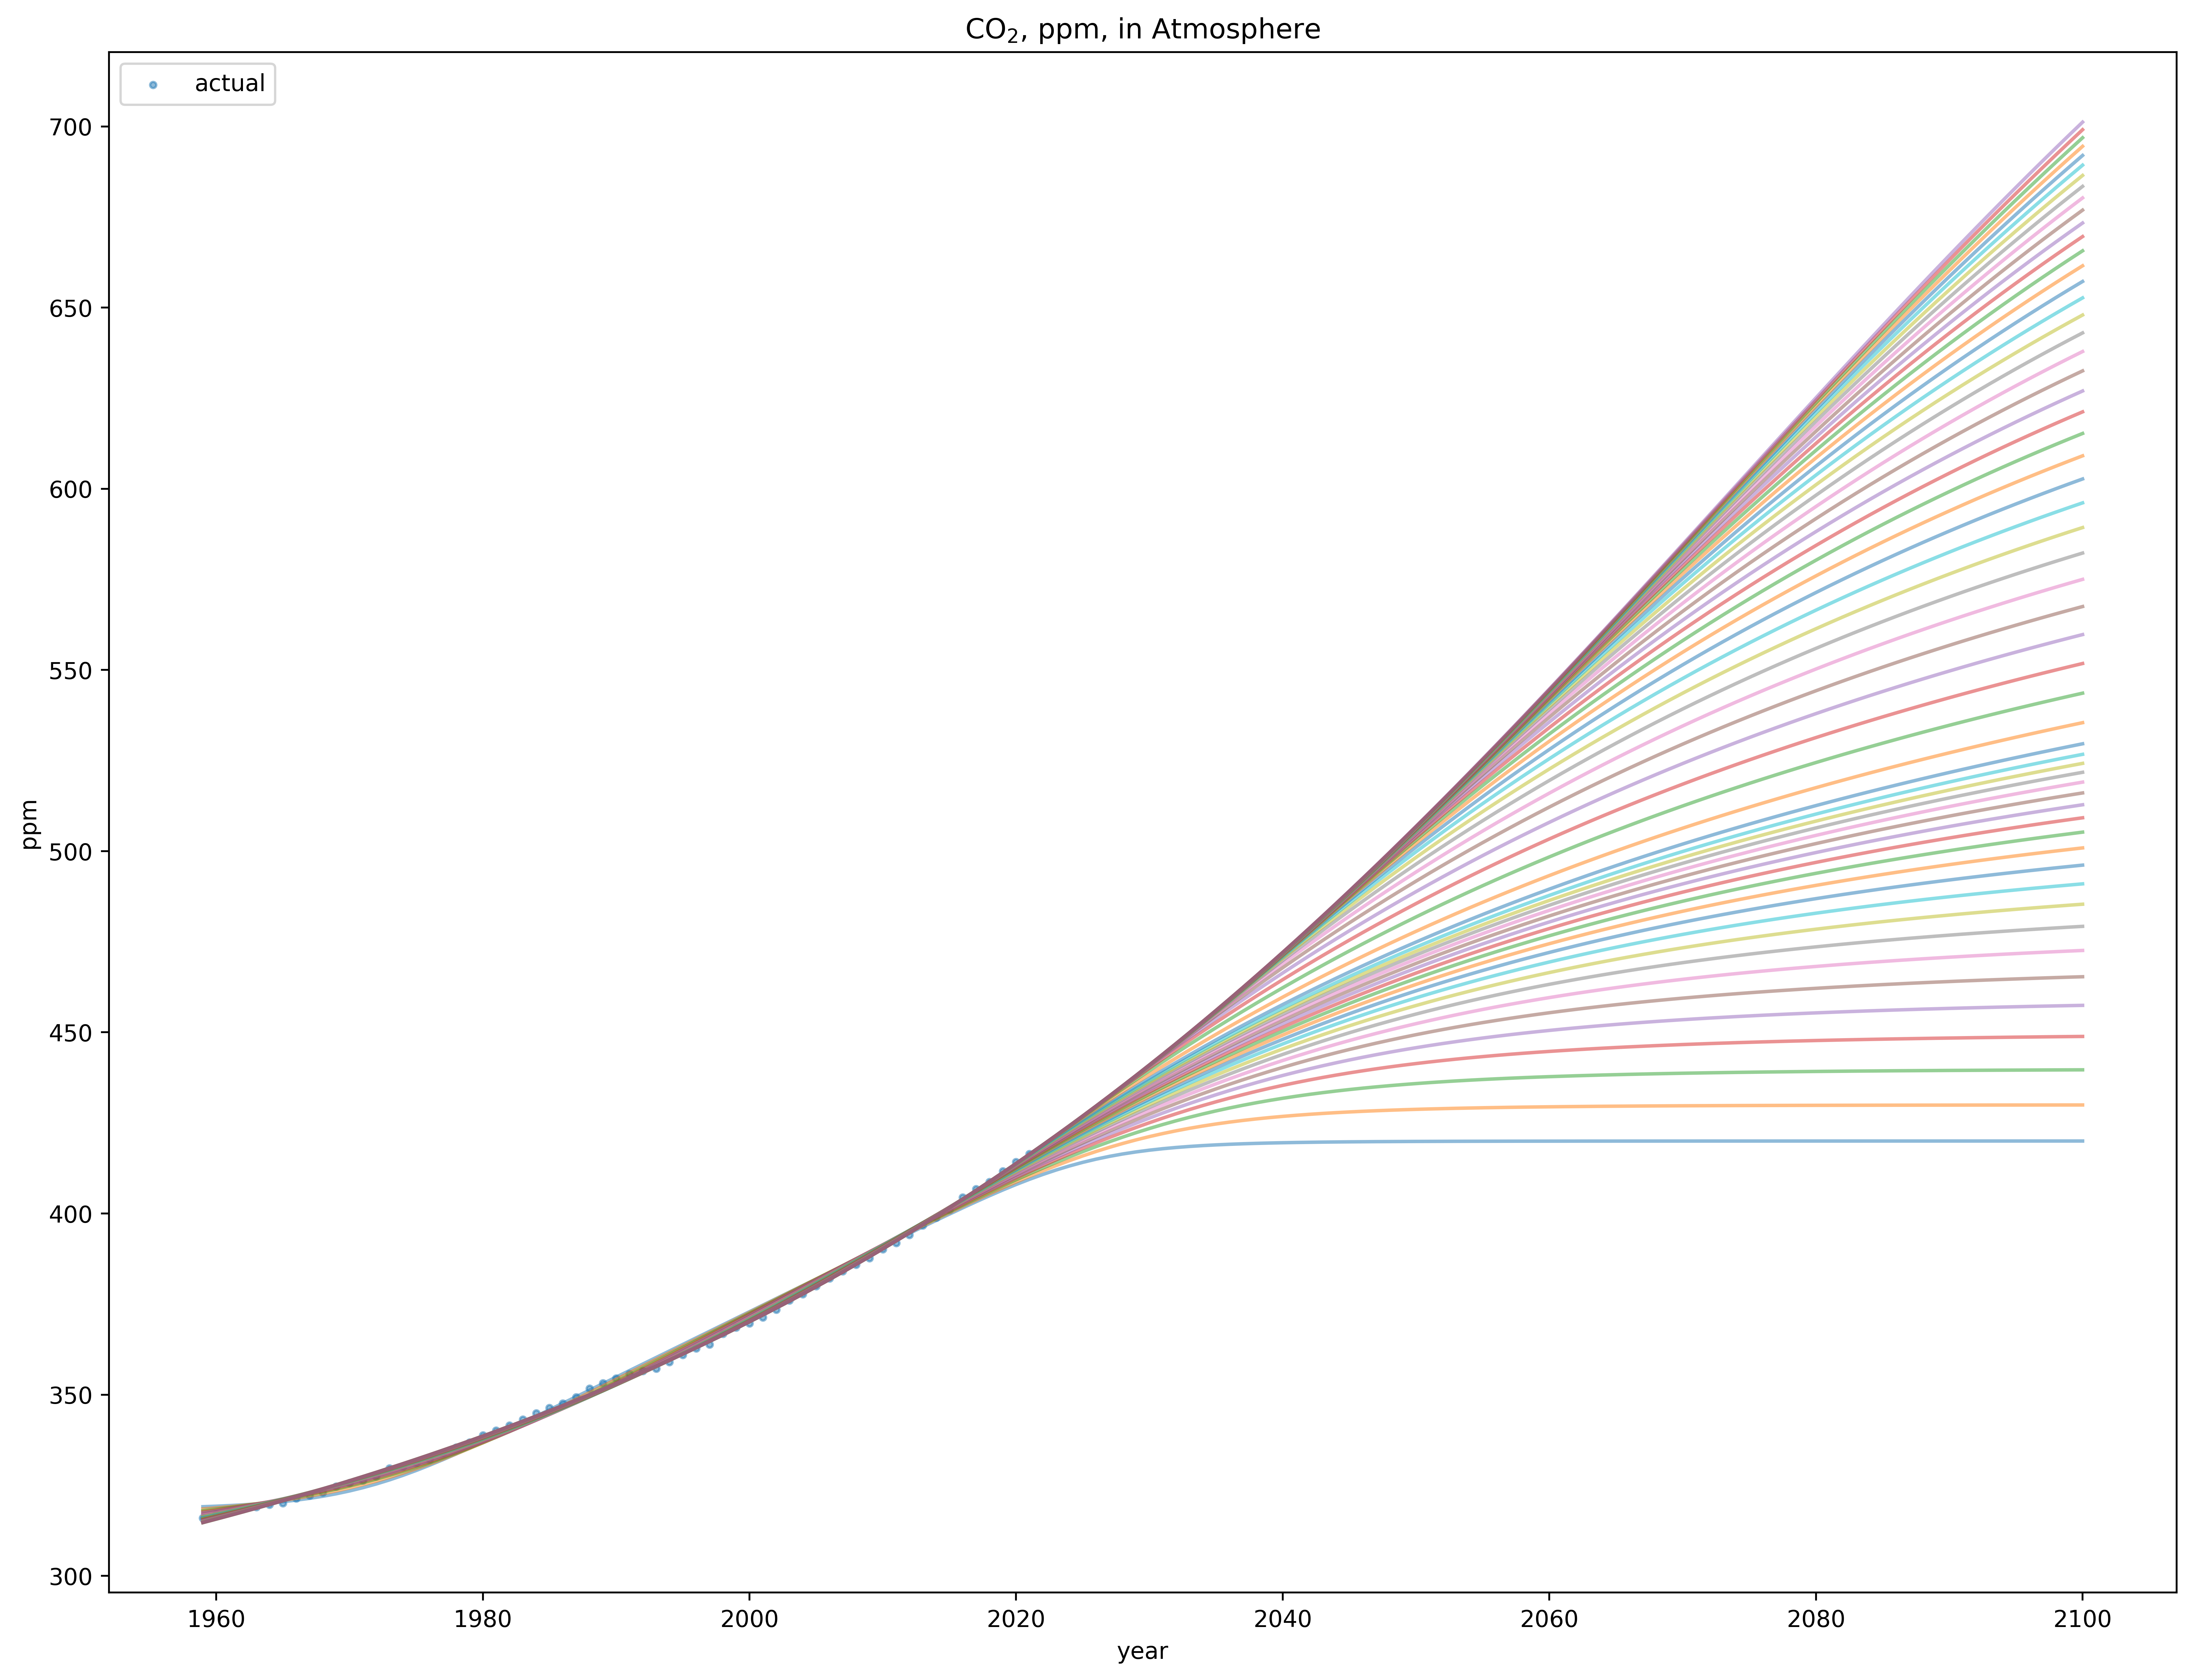
\includegraphics[width=\textwidth]{co2_sigm_all}%
            \caption{Sigmoid Functions with Different Limits}
            \label{fig:co2_sigm_all}
        \end{minipage}
    \end{figure}

    A limit at 565\si{ppm} obviously prevents the model from every reaching a 685\si{ppm} prediction. Therefore, a longer-term limit of 960\si{ppm} is used to predict the CO\textsubscript{2} level until 2100. This model predicts CO\textsubscript{2} levels to reach 685\si{ppm} in 2096. This is a reasonable limit because the predictions fall between the exponential and Prophet (explored below) models.


    \subsection{Prophet}
    Prophet is a an advanced time-series forecasting model developed by Facebook.
    Its selling points are the ability to produce multi-part models that fit complex trends as well as seasonality.
    Prophet is fast and generally maintains a high accuracy when predicting values.
    It can be used in a range of different contexts and it is robust to outliers, shifts in the overall trend and missing data.
    A Prophet model is similar to a Generalized Additive Model (reference):
%
    \begin{equation}
        f(x) = g(x) + s(x) + h(x) + \epsilon
    \end{equation}
%
    where
    $g$ is the trend (made of piecewise linear or logistic functions),
    $s$ captures seasonal patterns,
    $h$ captures holiday (one-off) effects, and
    $\epsilon$ is the remaining noise-like error unaccounted for by the model.

    The model follows a Bayesian approach, where the prior distribution is specified; the parameters are then tuned for the model to better fit the data set. The piecewise trend consists of change-points, which are automatically selected; an upper bound can be set with a logistic function. The seasonal patterns involve Fourier series, where the default orders for annual and weekly seasonality are set to 10 and 3 respectively. Holiday effects are extra parameters designed to take into account public holidays.

    While Prophet is able to fit to existing data with near-perfect accuracy, its future predictions are a linear extension of the latest trend - a projection of approximately 2.4\si{ppm} increase per year. This is a reasonable prediction, but it does not reach 685\si{ppm} within the next century. Summary of the model is presented in Figure~\ref{fig:co2_prophet} and Table~\ref{tab:co2_prophet_err}.

    \begin{table}[h]
        \begin{minipage}{0.7\linewidth}
            \centering
            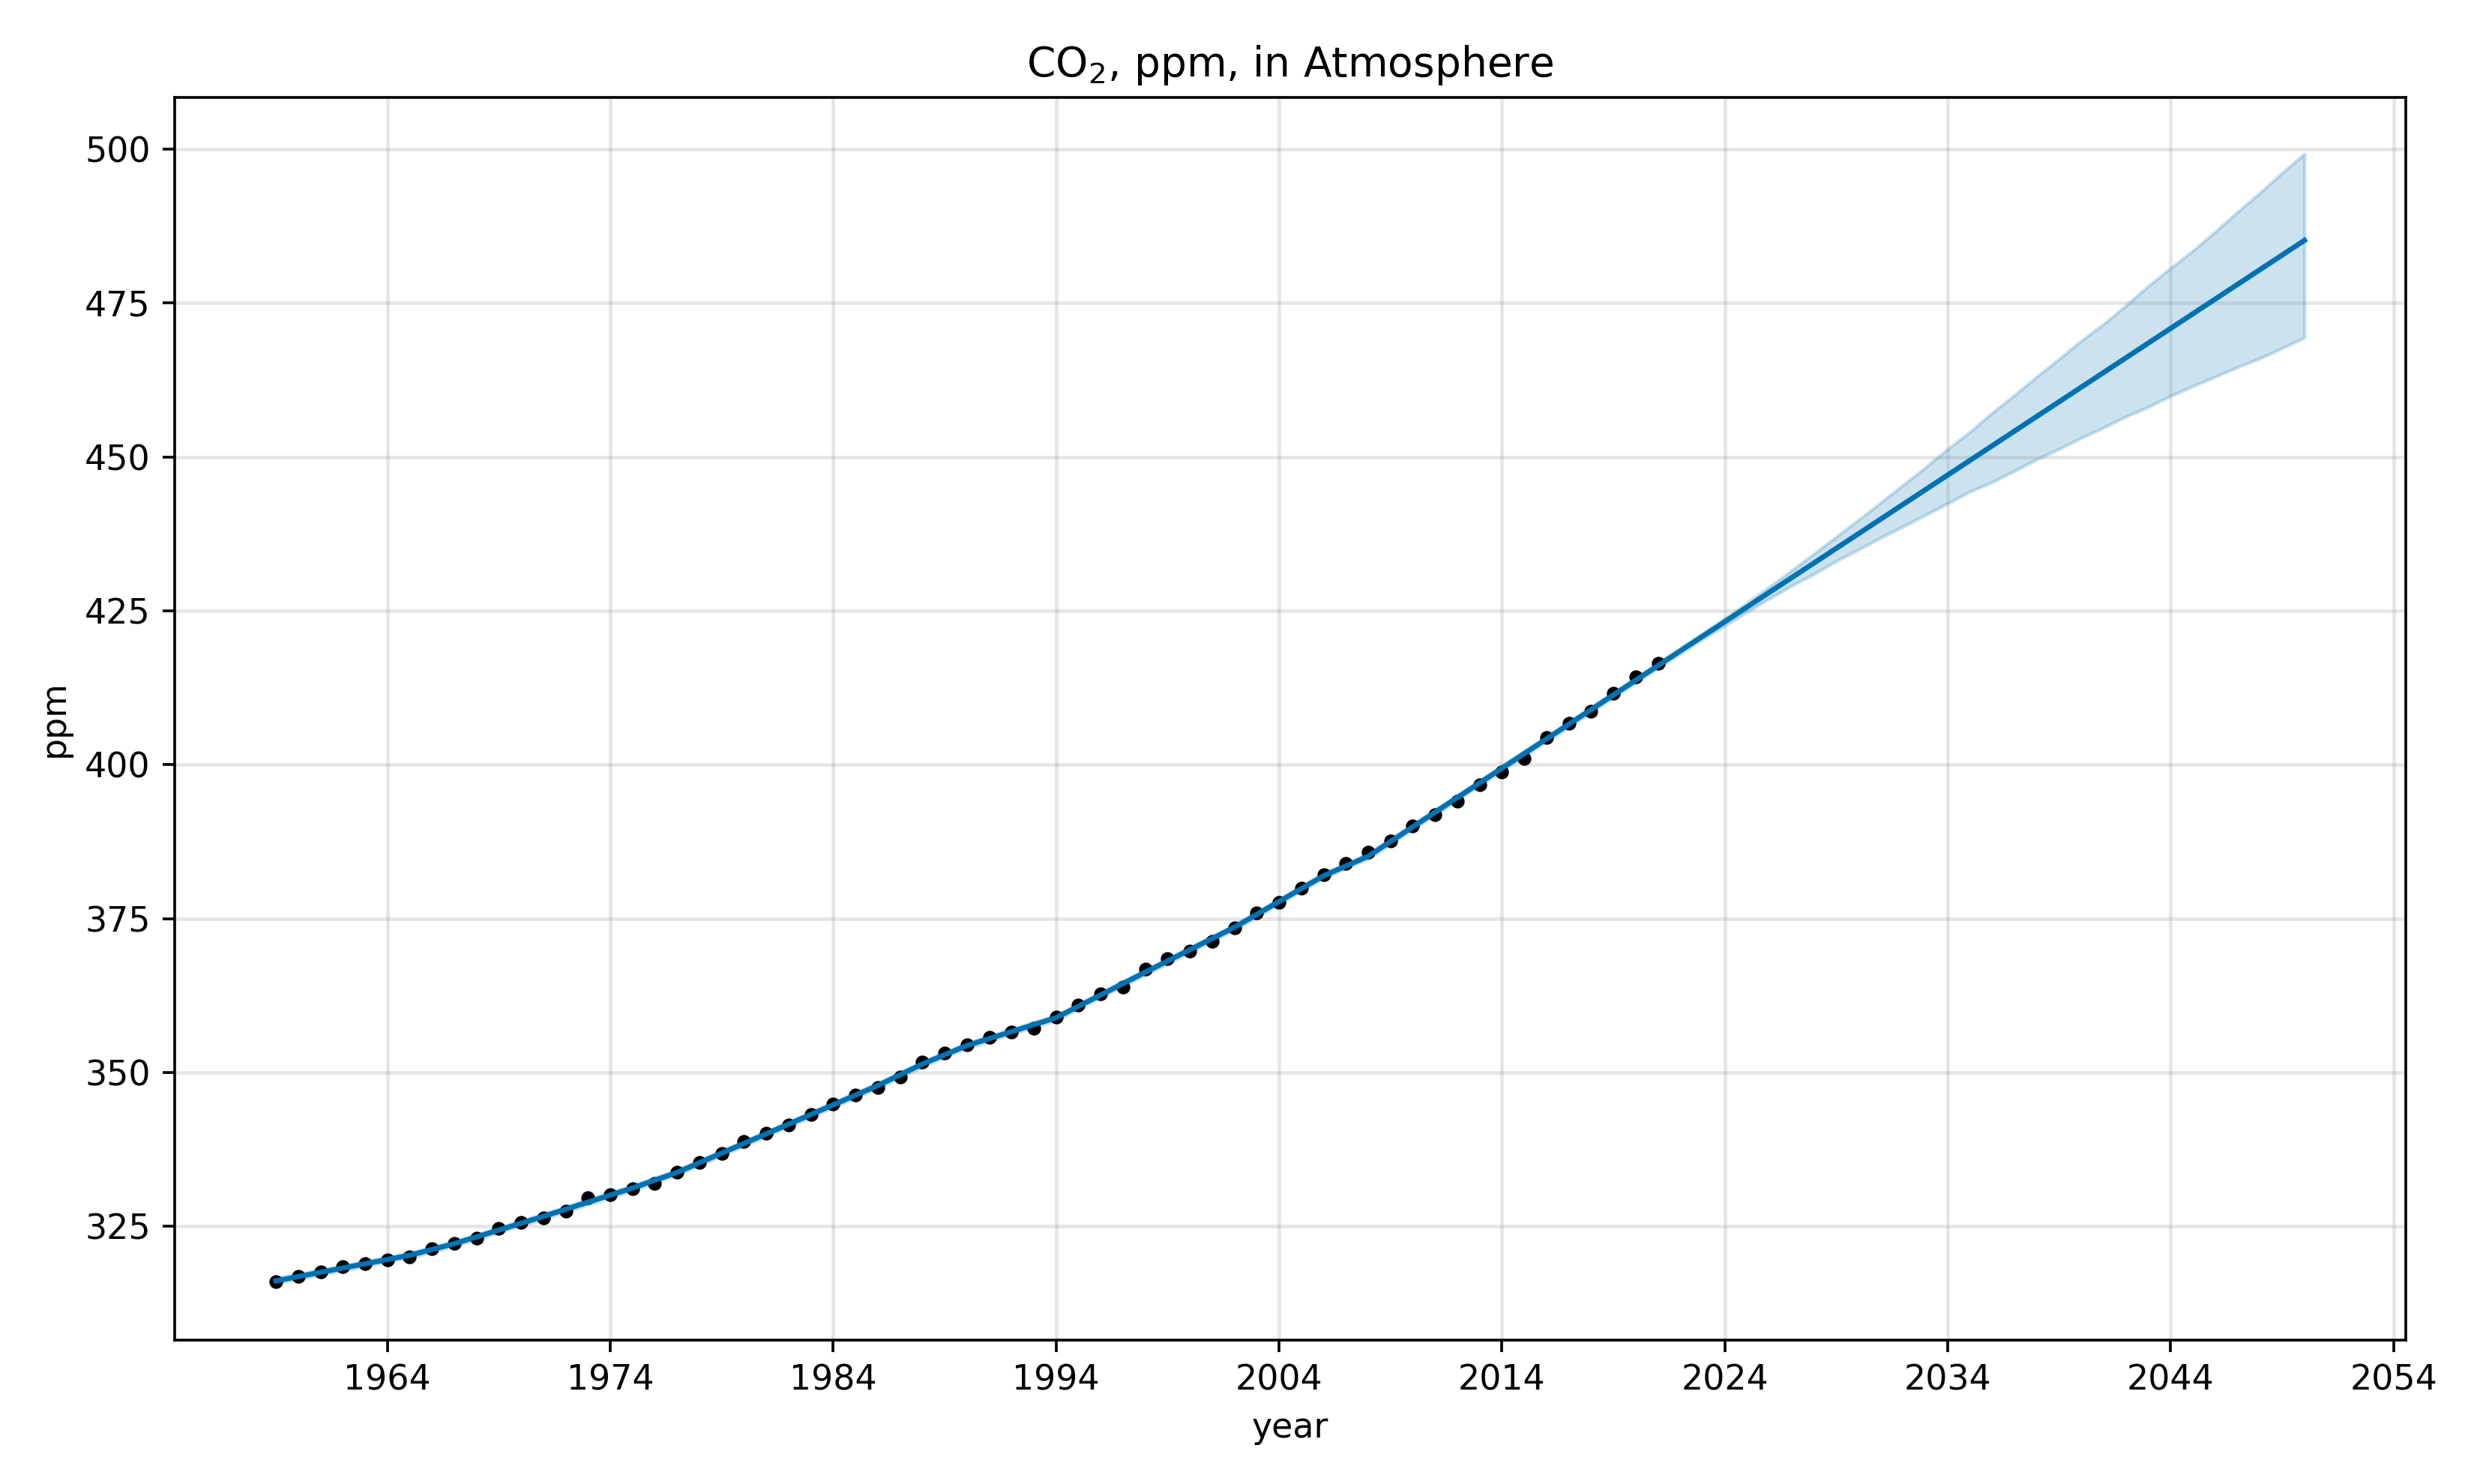
\includegraphics[width=\textwidth]{co2_prophet}%
            \captionof{figure}{Graph of Prophet}
            \label{fig:co2_prophet}
        \end{minipage}%
        \begin{minipage}{0.3\linewidth}
            \centering
            \begin{tabular}{ll}
                \toprule
                Metric               & Value   \\
                \midrule
                MSE                  & 0.10309 \\
                RMSE                 & 0.32108 \\
                MAE                  & 0.25507 \\
                PCC                  & 0.99994 \\
                R\textsuperscript{2} & 0.99988 \\
                CVAR                 & 890.82  \\
                \bottomrule
            \end{tabular}
            \vspace{8pt}
            \caption{Error Metrics for Prophet}
            \label{tab:co2_prophet_err}
        \end{minipage}
    \end{table}


    \subsection{ARIMA}
    An additional time-series prediction model that was investigated was ARIMA, which is based on ARMA (AutoRegressive Moving Average). These models are widely used in datasets that demonstrate non-stationarity, where the series\textquotesingle statistical properties such as mean, variance and autocorrelation change over time. ARMA assumes the input data to be stationary, so any non-stationary data has to be made stationary through a reversible process. Usually, the transformation involves finding the general trend with methods such as regression and then using differencing to remove the trend from the dataset. With the trend eliminated, an ARMA model can then be constructed and its optimal parameters found.

    Another appropriate model to use in regards to the data set is ARIMA, which is an extension of ARMA. ARIMA models are generally denoted as ARIMA$(p, d, q)$ where
    $p$ is the number of Auto-Regressive (AR) terms,
    $d$ is the orders of differencing, and
    $q$ is the number of Moving Average (MA) terms.

    The functions AR(p) and MA(q) are defined below as:
    AR(p):

    \begin{tabular}{|*2{p{.45\textwidth}|}}
        \hline
        AR(p):                       & MA(q):                   \\
        \quad ${\phi (B) X_t = w_t}$ & ${X_t = \theta (B) w_t}$ \\[\baselineskip]
        Where
        \begin{itemize}[nosep]
            \item ${\phi (B)}$ = Autoregressive operator
            \item ${X_t}$ = Inverse operator
            \item ${w_t}$ = White noise
        \end{itemize}
        &
        Where
        \begin{itemize}[nosep]
            \item ${\theta (B)}$ = Moving average operator
            \item ${X_t}$ = Inverse operator
            \item ${w_t}$ = White noise
        \end{itemize}
        \\
        \hline
    \end{tabular}

    Before tuning the parameters p and q, the number of differencing required to make the data stationary must be found out. To evaluate whether the current dataset is stationary, an Augmented Dickey-Fuller (ADF) test was performed.

    ADF tests expand on the original Dickey-Fuller test by including higher-order autoregressive processes to form the equation:
%
    \begin{equation}
        \Delta y_{t}=\alpha +\beta t+\gamma y_{t-1}+\delta _{1}\Delta y_{t-1}+\cdots +\delta _{p-1}\Delta y_{t-p+1}+\varepsilon _{t}
    \end{equation}
%
    where
    ${y_{t}}$ is the value of the time series at time t,
    ${\alpha}$ is a constant,
    ${\beta}$ is the coefficient of the trend, and
    $p$ is the lag order of the autoregressive process.

    The results of the ADF test applied on the given dataset is presented below:
%
    \begin{center}
        \begin{tabular}{ |c|c|c|c|}
            \hline
            \textbf{ADF Test Statistic}  & 5.506786113910213 & \textbf{Significance Level} & \textbf{Critical Value} \\
            \hline
            \textbf{P-Value}             & 1.0               & \textbf{1\%}                & -3.5463945337644063     \\
            \hline
            \textbf{No. of Lags Used}    & 2                 & \textbf{5\%}                & -2.911939409384601      \\
            \hline
            \textbf{No. of Observations} & 59                & \textbf{10\%}               & -2.5936515282964665     \\
            \hline
        \end{tabular}
    \end{center}

    The p-value obtained is greater than the significance level 0.05 and the ADF statistic is higher than any of the critical values, hence it can be concluded that the time series has a unit root and is non-stationary. The high p-value signifies that a high order of differencing will need to be used.

    To further confirm the data\textquotesingle s stationarity, autocorrelation and partial autocorrelation graphs were also used. AFC and PAFC functions are measures of correlation between past and present data, and indicate which past data values are most useful in predicting future ones. The results of these functions are then used to select the most optimal parameters for p and q. Both functions were applied on the given dataset and the graphed results displayed below:

    \begin{wrapfigure}{R}{0.6\textwidth}
        \centering
        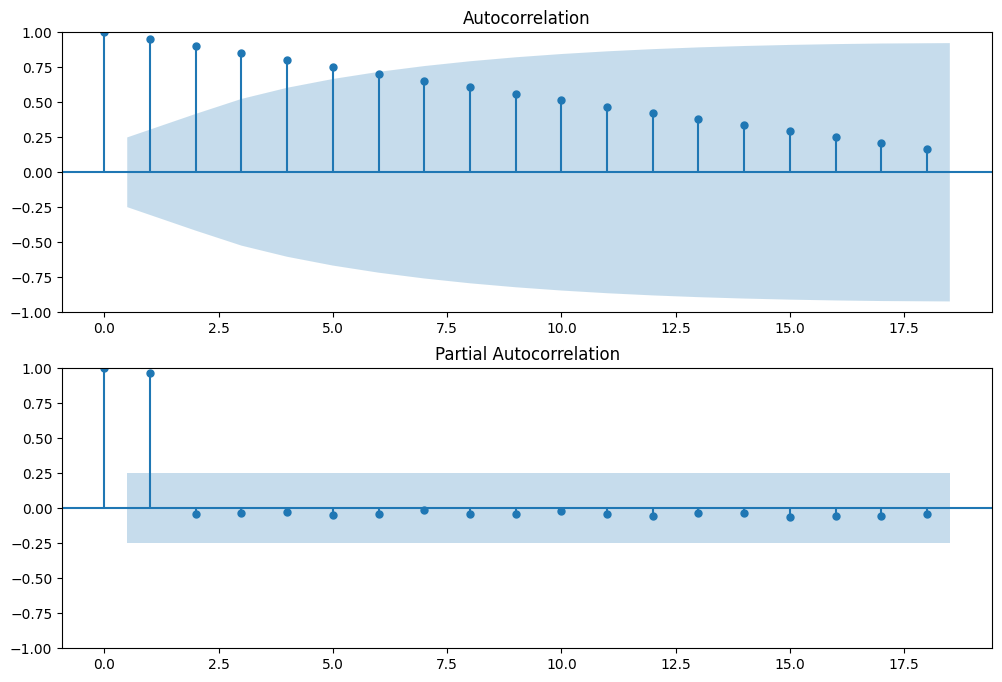
\includegraphics[width=0.6\textwidth]{pacf_acf}
        \caption{ACF and PACF of CO\textsubscript{2} data}
        \label{fig:pacf_acf}
    \end{wrapfigure}

    For both graphs the x-axis represents lag, whereas the y-axis indicates the correlation strength. ACF graphs represent the correlation between data values that are n intervals apart. PACF graphs are similar in that they represent the same information, however they also account for the values of the intervals in between.

    The correlation that can be seen in the ACF graph is negative, indicating that large current values correspond with small values at the specified lag. The absolute correlation values represent the strength of the relationship; to construct an ARIMA model, the expected trend of these values should be random. In this case, the initial relationship between past and present values is strong, but gradually decreases over lags, indicating a clear trend of decreasing correlation strength.

    If the autocorrelation follows a random non-linear trend, then AR(p) and MA(q) can be applied to the graphed functions to obtain the optimal parameter values for p and q.
    However, this is only assuming the data does not have a trend or seasonality component, which does not apply to the given dataset.

    The autocorrelation trend as well as the high order of differencing required to transform the data to stationary (as seen in the ADF test) both demonstrate that the given dataset is unsuitable for constructing an ARIMA model, and therefore this prediction model has been rejected and will not be used as part of the predicted CO\textsubscript{2} and temperature values.



    \section{CO\textsubscript{2} - Model Evaluation}

    \subsection{Procedure}

    To rank the 4 accepted predictive models on their mathematical accuracy, the following error metrics are to be calculated for each model and then compared with each other:
%
    \begin{tabular}{|*2{p{.5\textwidth}|}}
        \hline
        \textbf{Scale-dependent Errors} & \textbf{Forecast Errors} \\
        \hline
        \begin{itemize}[nosep]
            \item MSE (Mean Squared Error)
            \item RMSE (Root Mean Squared Error)
            \item MAE (Mean Absolute Error)
            \item PCC (Pearson\textquotesingle s Correlation Coefficient)
            \item ${R^2}$ (Coefficient of Determination)
            \item Covariance
        \end{itemize}
        &
        \begin{itemize}[nosep]
            \item Seperation of known values into testing and training data
        \end{itemize}
        \\
        \hline
    \end{tabular}

    \noindent \textbf{Separation of Known Values into Testing and Training data}

    75\% of known data values are allocated to the testing data group, remaining 25\% are allocated to the training group. The predictive model will take in the training group data values as its sole input, and will predict the remaining 25\%. The model\textquotesingle s predicted values are then to be compared with the training group\textquotesingle s values and the forecast errors obtained.
    A forecast error is defined as the difference between an observed and its forecasted value; the formula for a single forecast error can be modified to suit multiple data values, and it is denoted by the following equation:
%
    \begin{equation}
        e_{T+h} = y_{T+h} - \hat{y}_{T+h|T}
    \end{equation}
%
    where
    ${e_{T+h}}$ is the forecast error,
    ${y_{T+h}}$ is the actual value of the h-step observation, and
    ${\hat{y}_{T+h|T}}$ is the actual value of the h-step forecast.

    The equation was again modified to find the sum of all the forecast errors, this was then applied to each model to construct the table below:
%
    \begin{center}
        \begin{tabular}{ |c|c|c|c|c|}
            \hline
            & \textbf{Linear} & \textbf{Exponential} & \textbf{Sigmoid} & \textbf{Prophet} \\
            \hline
            \textbf{Forecast RMSE} & 11.660          & 0.37768                & 0.41312            & 3.5618            \\
            \hline
        \end{tabular}
    \end{center}

    \begin{figure}
        \centering
        \begin{minipage}{0.5\linewidth}
            \centering
            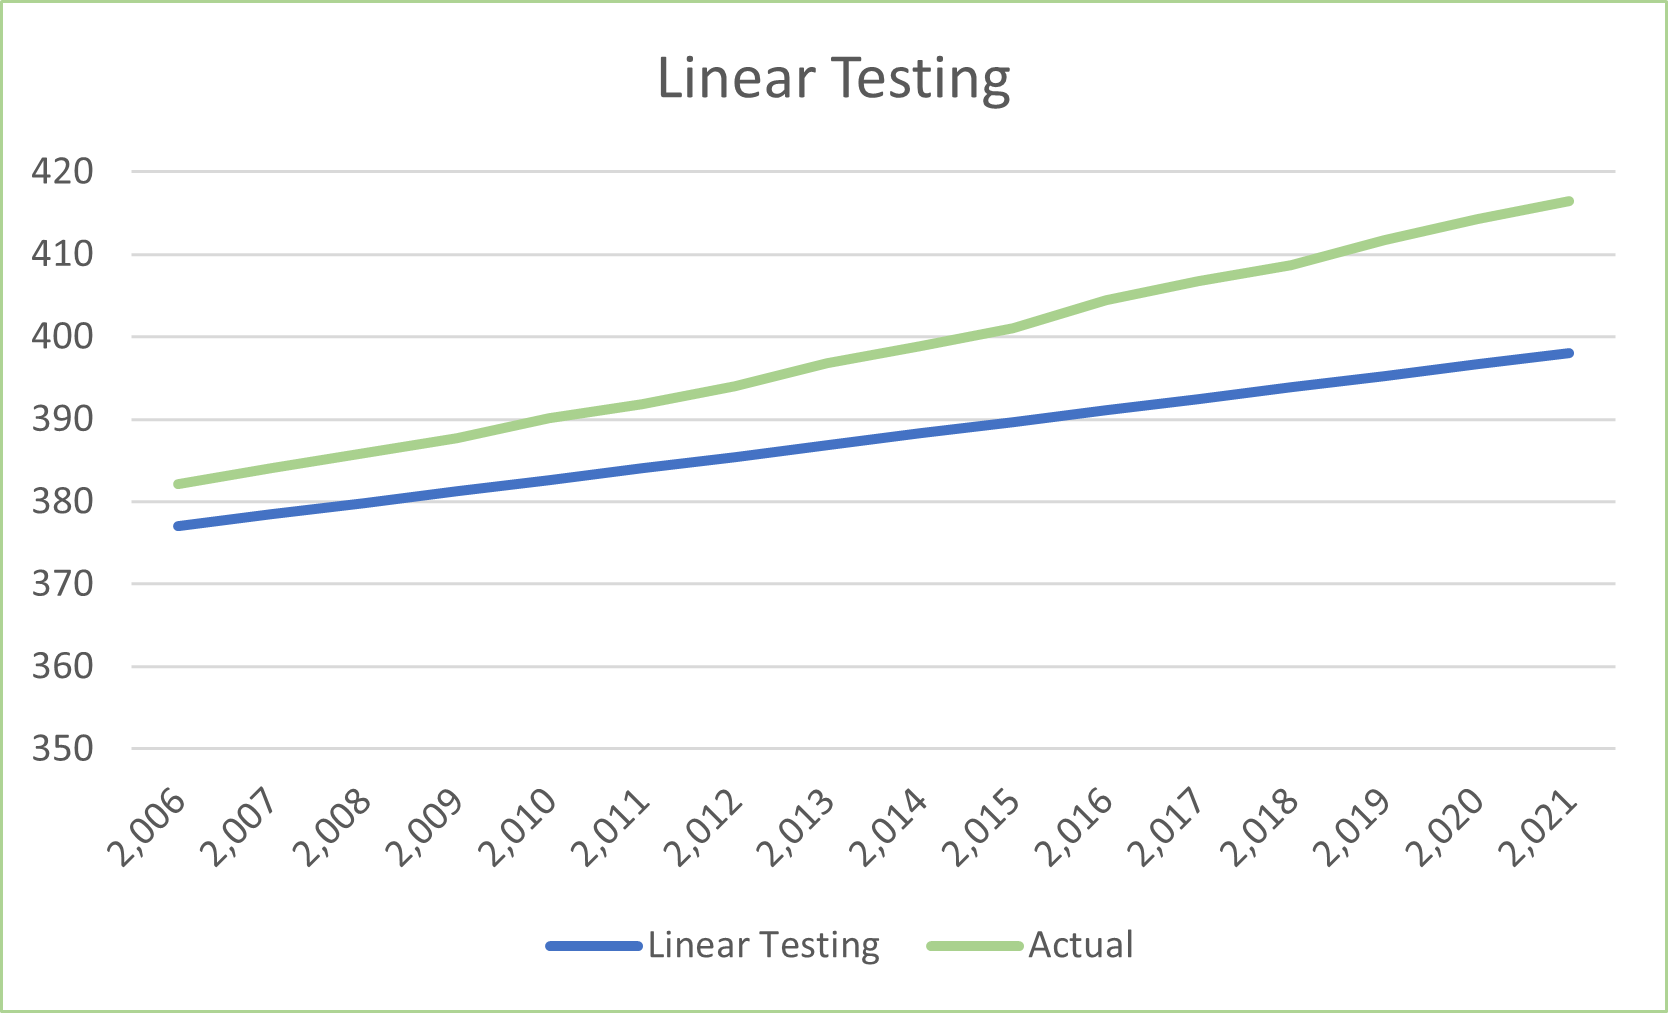
\includegraphics[width=\textwidth]{linear_testing}
        \end{minipage}%
        \begin{minipage}{0.5\linewidth}
            \centering
            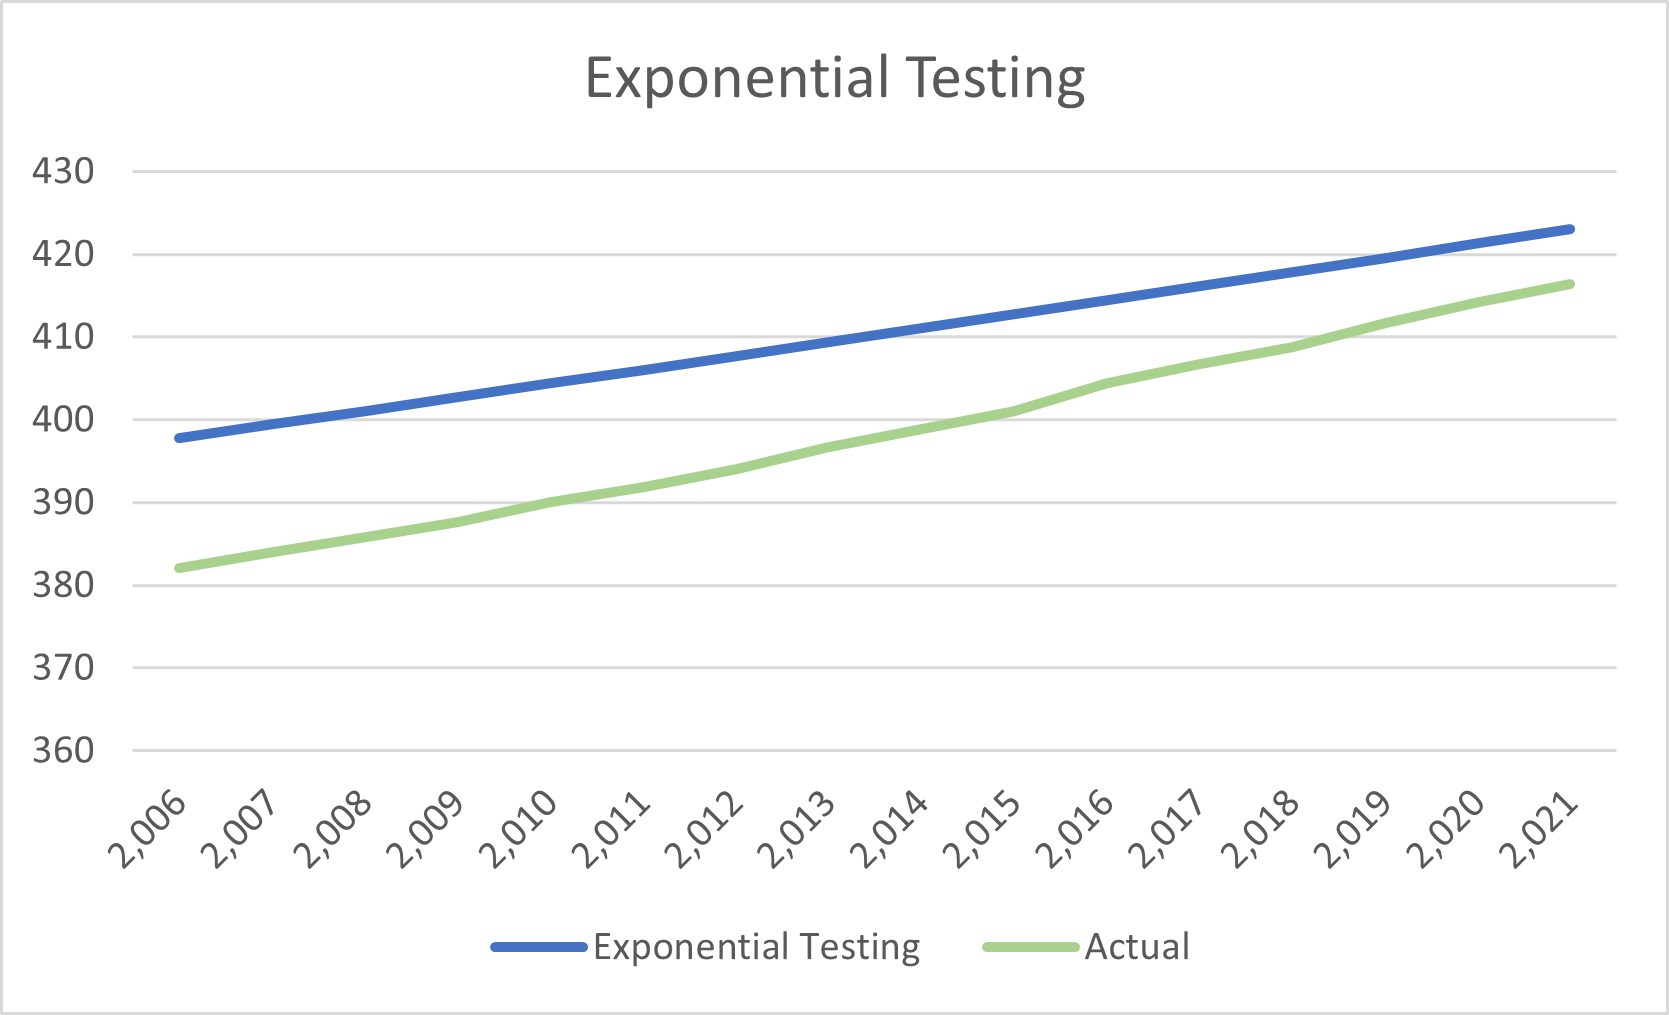
\includegraphics[width=\textwidth]{exponential_testing}
        \end{minipage}
    \end{figure}%
    \begin{figure}
        \centering
        \begin{minipage}{0.5\linewidth}
            \centering
            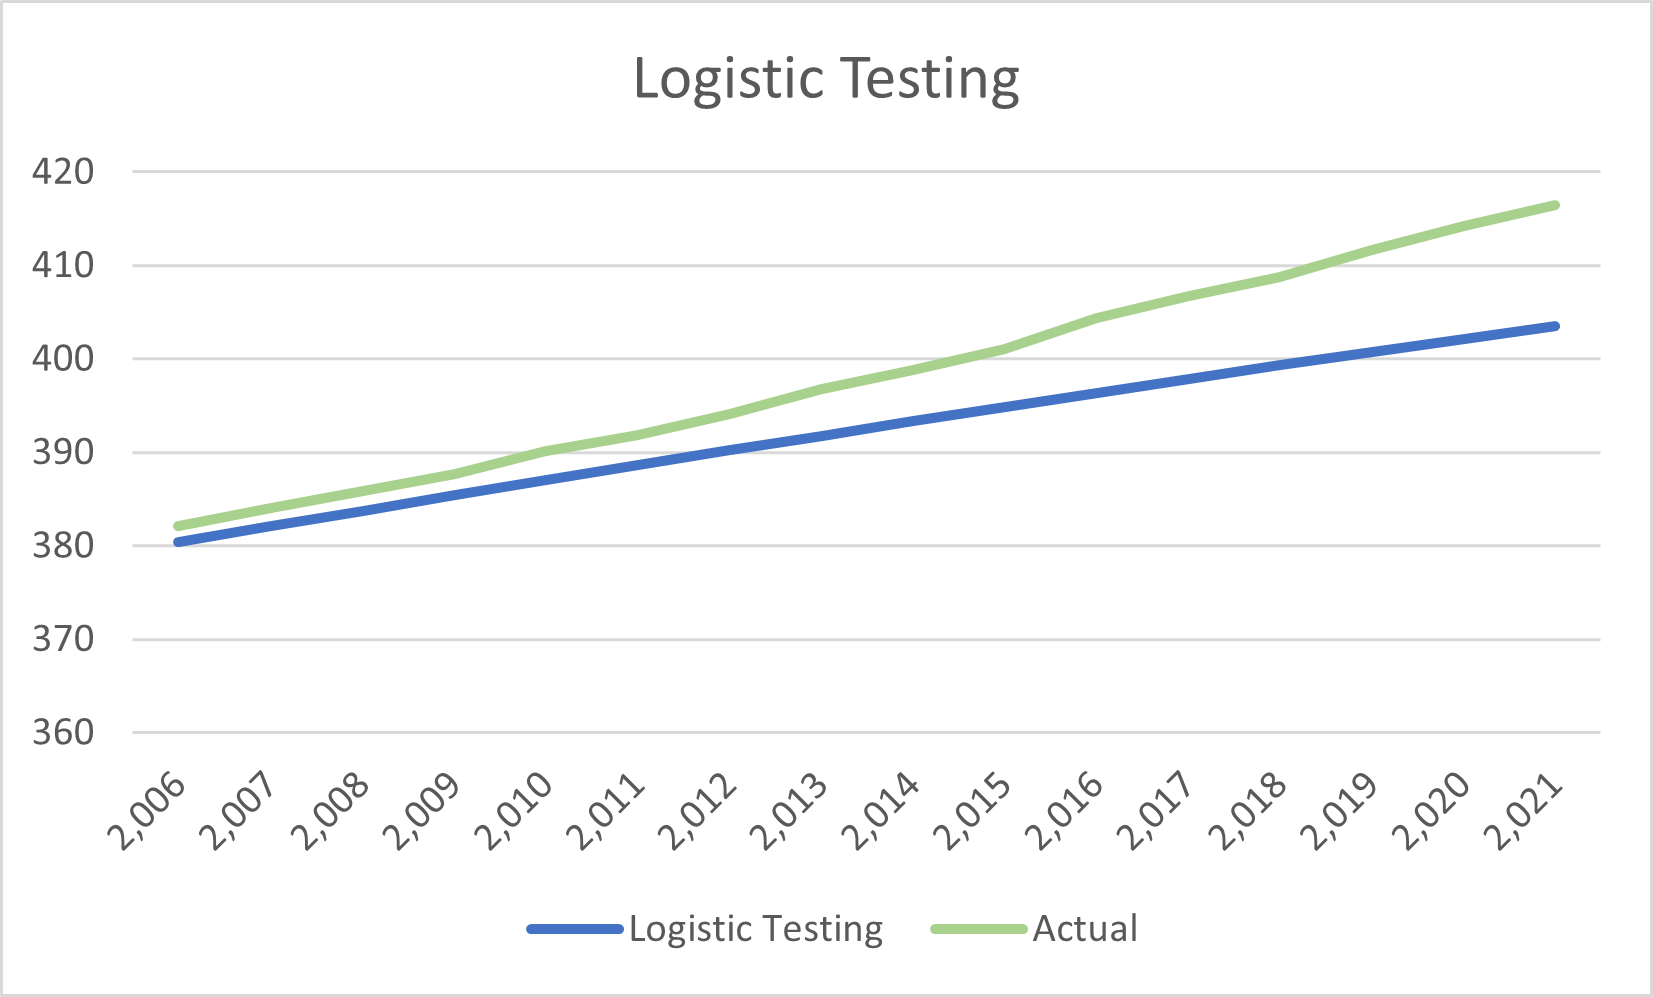
\includegraphics[width=\textwidth]{logistic_testing}
        \end{minipage}%
        \begin{minipage}{0.5\linewidth}
            \centering
            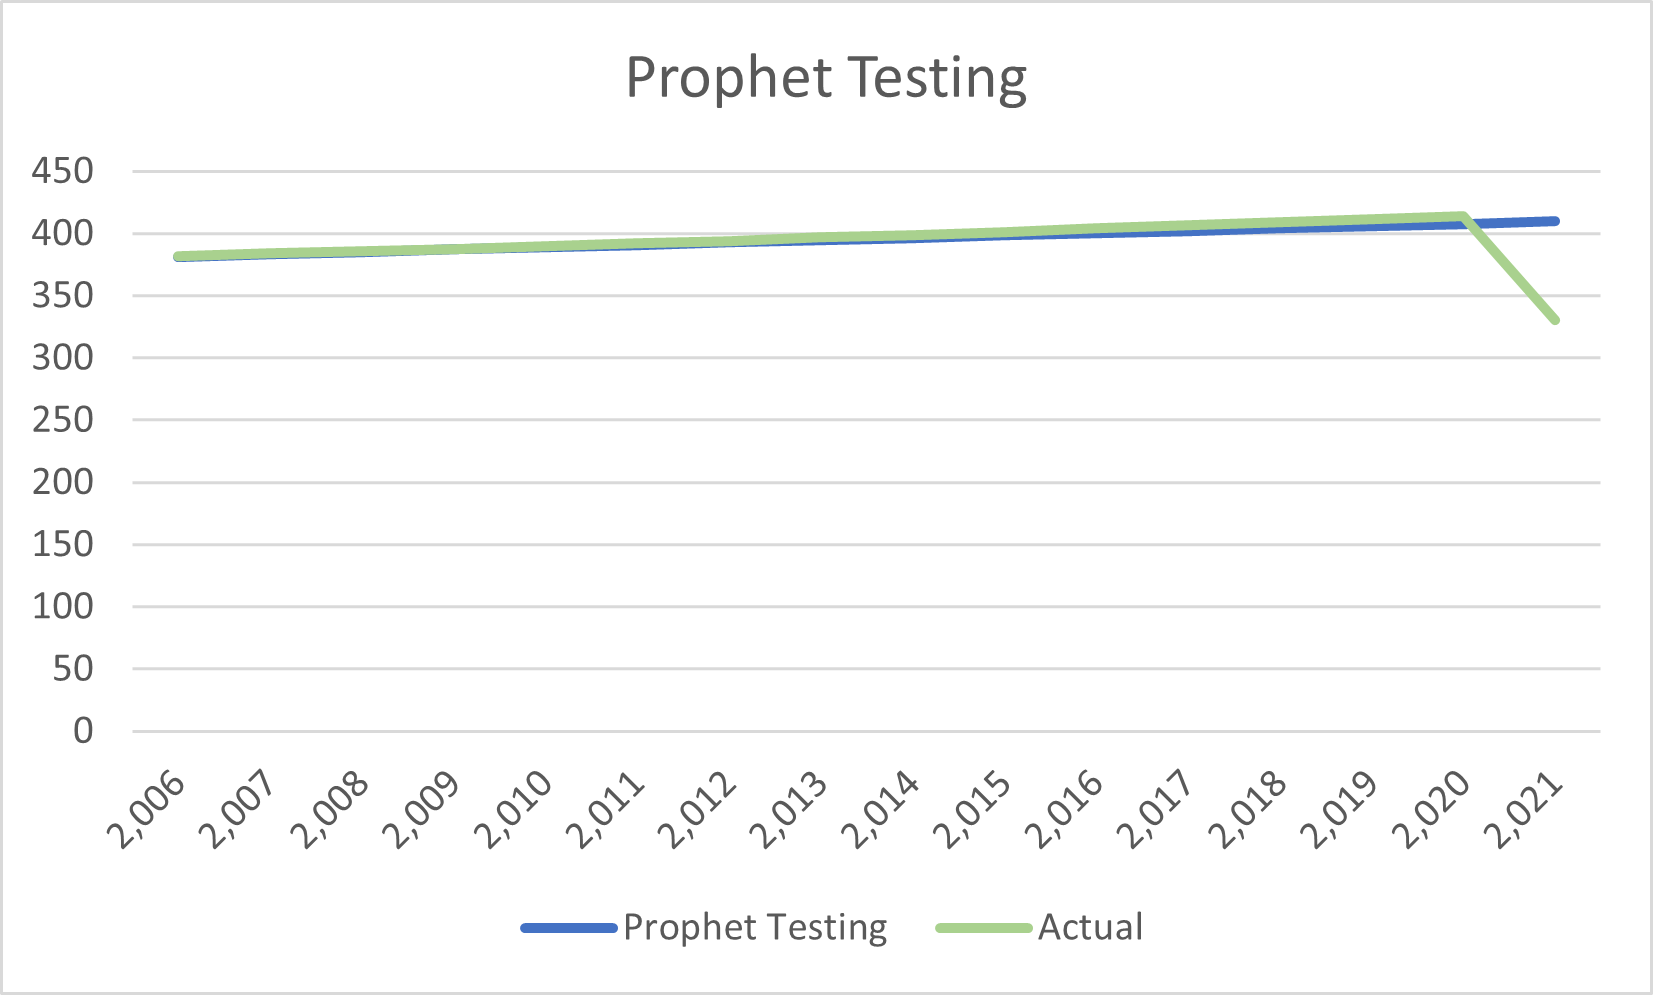
\includegraphics[width=\textwidth]{prophet_testing}
        \end{minipage}
    \end{figure}


    It is important to note that although a model may fit the testing data well, it does not necessarily mean the model will forecast well, therefore it is important to take the other error metrics into consideration.


    \subsection{Accuracy Analysis}

    \subsubsection*{MSE}
    Mean Squared Error (MSE) is a measure of the quality of a predictor or of an assessor, its definition differing accordingly. It is the average squared distance between the actual and predicted values, measuring the variance of the residuals. In this case, only the quality of the predictor is to be assessed. It involves taking the average squared distance between the actual and predicted values, measuring the variance of the residuals. The within-sample MSE of a predictor can then be denoted as:
%
    \begin{equation}
        \operatorname {MSE} ={\frac {1}{n}}\sum _{i=1}^{n}\left(Y_{i}-{\hat {Y_{i}}}\right)^{2}
        \label{eq:MSE}
    \end{equation}
%
    where
    ${\frac {1}{n}\sum _{i=1}^{n}}$ calculates the mean (across all data points) and
    ${\left(Y_{i}-{\hat {Y_{i}}}\right)^{2}}$ is the squares of the difference between the actual and predicted values, or the error.

    MSE also has a differentiable graph so it makes it easier to perform mathematical operations in comparison to MAE. MSE is more sensitive to outliers compared to MAE\@.

    \subsubsection*{RMSE}
    Root Mean Squared Error (RMSE) is the square root of the MSE, measuring the standard deviation of the residuals. The higher the RMSE value, the larger the deviation between actual and predicted values. By proxy, the lower the RMSE value, the lower the deviation, hence the model is more accurate. Building on the MSE~\eqref{eq:MSE} formula, RMSE can be denoted as:
%
    \begin{equation}
        \operatorname {RMSE} = \sqrt{MSE}
    \end{equation}

    When outliers are exponentially rare, such as this situation, RMSE is generally preferred over MSE as it provides a better evaluation of model performance, as it uses the same units as the Y axis (CO\textsubscript{2} emissions).

    \subsubsection*{MAE}
    Mean Absolute Error (MAE) is the sum of the absolute difference between the actual and predicted values. A perfect prediction model would yield a 0 as its MAE value. The further away from 0 the MAE value is, the more errors the model makes and hence the less accurate the model is. The formula to calculate MAE is denoted as:
%
    \begin{equation}
        \displaystyle {MAE} ={\frac {\sum _{i=1}^{n}\left|y_{i}-x_{i}\right|}{n}}
    \end{equation}
%
    where
    ${\sum _{i=1}^{n}\left|y_{i}-x_{i}\right|}$ is the sum of absolute error and
     $n$ is the Number of data points.

    \subsubsection*{PCC, R\textsuperscript{2}, AND COVARIANCE}
    The last 3 error metrics are explained in further detail when exploring the relationship between temperature and CO\textsubscript{2} emissions



    \section{CO\textsubscript{2} - Results \& Conclusions}

    \subsection{Forecast Results}

    Figure~\ref{fig:co2_all} summarizes all above models in one graph.
    The horizontal line marks 685\si{ppm}.

    \begin{figure}[h]
        \centering
        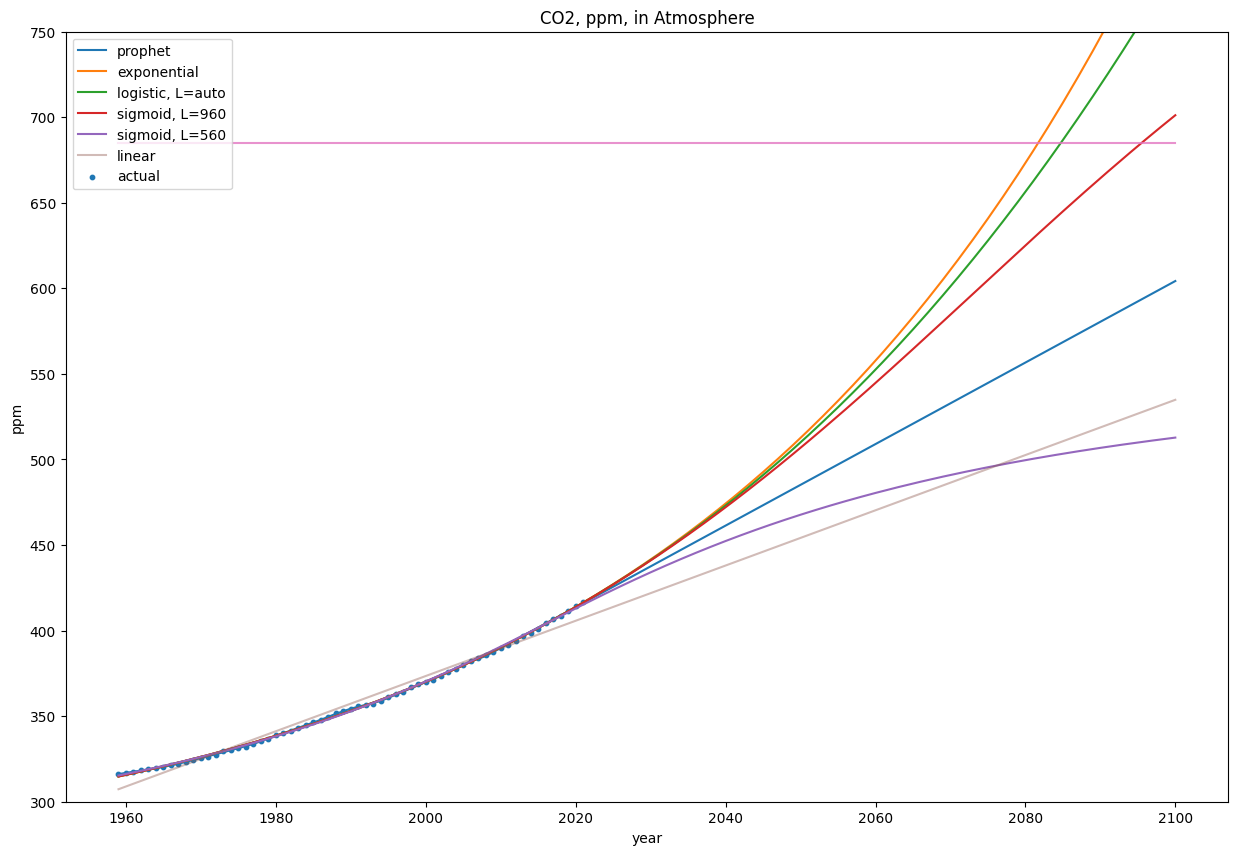
\includegraphics[width=\linewidth]{co2_pred_all}
        \caption{Graph of all Models}
        \label{fig:co2_all}
    \end{figure}


    The MSE, RMSE, MAE, PCC, R\textsuperscript{2} and covariance were calculated for each accepted model, rounded to 5 s.f., and compiled into a results table below. For each error metric, the model with the value closest to and furthest from a perfect value were highlighted:

    \begin{center}
        \begin{tabular}{ |c|c|c|c|c|}
            \hline
            & \textbf{Linear} & \textbf{Exponential} & \textbf{Sigmoid} & \textbf{Prophet} \\
            \hline
            \textbf{MSE}        & 15.376          & 0.47977              & 0.61002          & 0.10310          \\ \hline
            \textbf{RMSE}       & 3.9212          & 0.69266              & 0.78104          & 0.32109          \\ \hline
            \textbf{MAE}        & 3.1920          & 0.56081              & 0.66350          & 0.25507          \\ \hline
            \textbf{PCC}        & 0.99119         & 0.99973              & 0.99965          & 0.99994          \\ \hline
            \textbf{R\textsuperscript{2}}    & 0.98246         & 0.99945              & 0.99930          & 0.99990          \\ \hline
            \textbf{Covariance} & 875.32          & 890.45               & 889.87           & 890.82           \\ \hline
        \end{tabular}
    \end{center}

    For each model, the year at which 685ppm was reached and the range from 2050 was found to construct the following table:

    \begin{table}
        \centering
        \begin{tabular}{ |c|c|c|c|c|}
            \hline
            & \textbf{Linear} & \textbf{Exponential} & \textbf{Sigmoid} & \textbf{Prophet} \\
            \hline
            \textbf{Year (at which 685ppm is reached)} & 2193            & 2081                 & 2096             & 2134             \\
            \hline
            \textbf{Range (from 2050)}                 & +143            & +31                  & +46              & +84              \\
            \hline
        \end{tabular}
        \caption{Different Models\textquotesingle~Predictions to reach 685ppm}
        \label{tab:co2_685}
    \end{table}

    The train-test data split procedure demonstrated that the exponential model has the least amount of forecasting errors.
    However, Prophet has the best error metrics, such as the lowest MSE and highest R\textsuperscript{2}. However, this improvement is small over the exponential model and is explained by Prophet's ability to fit to arbitrary trends where it was able to capture irregularities in the data; essentially over-fitting.

    Overall, even if by a small margin, as the Prophet model better fulfills the above criteria, it is deemed to be the most accurate out of the accepted models chosen and tested. This decision is reinforced by the model’s use in major companies; additional studies have also demonstrated Prophet’s high accuracy in predictions. A major disadvantage to the model however is its speed, as the run time to process a single item is ~60ms. In this situation, this disadvantage can be overlooked, as the data set was small enough so as not to cause time issues.


    \subsection{Comparison with External Claims}

    With all relevant models fully constructed, a conclusion can be provided in response to claims by external sources.


    \subsubsection*{NOAA: 2004 observed largest increase yet}

    Quoted from the problem statement: the ``March 2004 increase of CO\textsubscript{2} resulted in a larger increase than observed over any previous 10-year period''.

    Before attempting to verify this claim, ambiguities in the meaning of a ``larger increase than observed over any previous 10-year period'' must be clearly defined.
    This statement contains two parts: ``larger increase than [previously] observed'' and ``any previous 10 year period''.
    How a comparative change metric for any 10-year period is left to interpretation.
    In the end, two reasonable quantitative approaches were adopted, both of which perform calculations on pre-2004 data, 10 consecutive years at a time, to generate a metric that encapsulates the change of CO\textsubscript{2} levels for that decade.


    \noindent\size{12}{\textbf{Comparing to decadal changes}}

    In this approach, a simple method was used to calculate the net percentage change between any two years for CO\textsubscript{2} levels. The following equation was used,
%
    \begin{equation}
        \displaystyle \% \triangle CO_2 = \frac{C_f - C_i}{C_i} \times 100
    \end{equation}
%
    where
    $C_f$ is the CO\textsubscript{2} level in the final year of the decade and
    $C_i$ is the CO\textsubscript{2} level in the initial year of the decade.

    This computation was carried out using a moving ten-year interval window, yielding a comparable measure of change for every preceding decade.

    \begin{wrapfigure}{R}{0.6\textwidth}
        \centering
        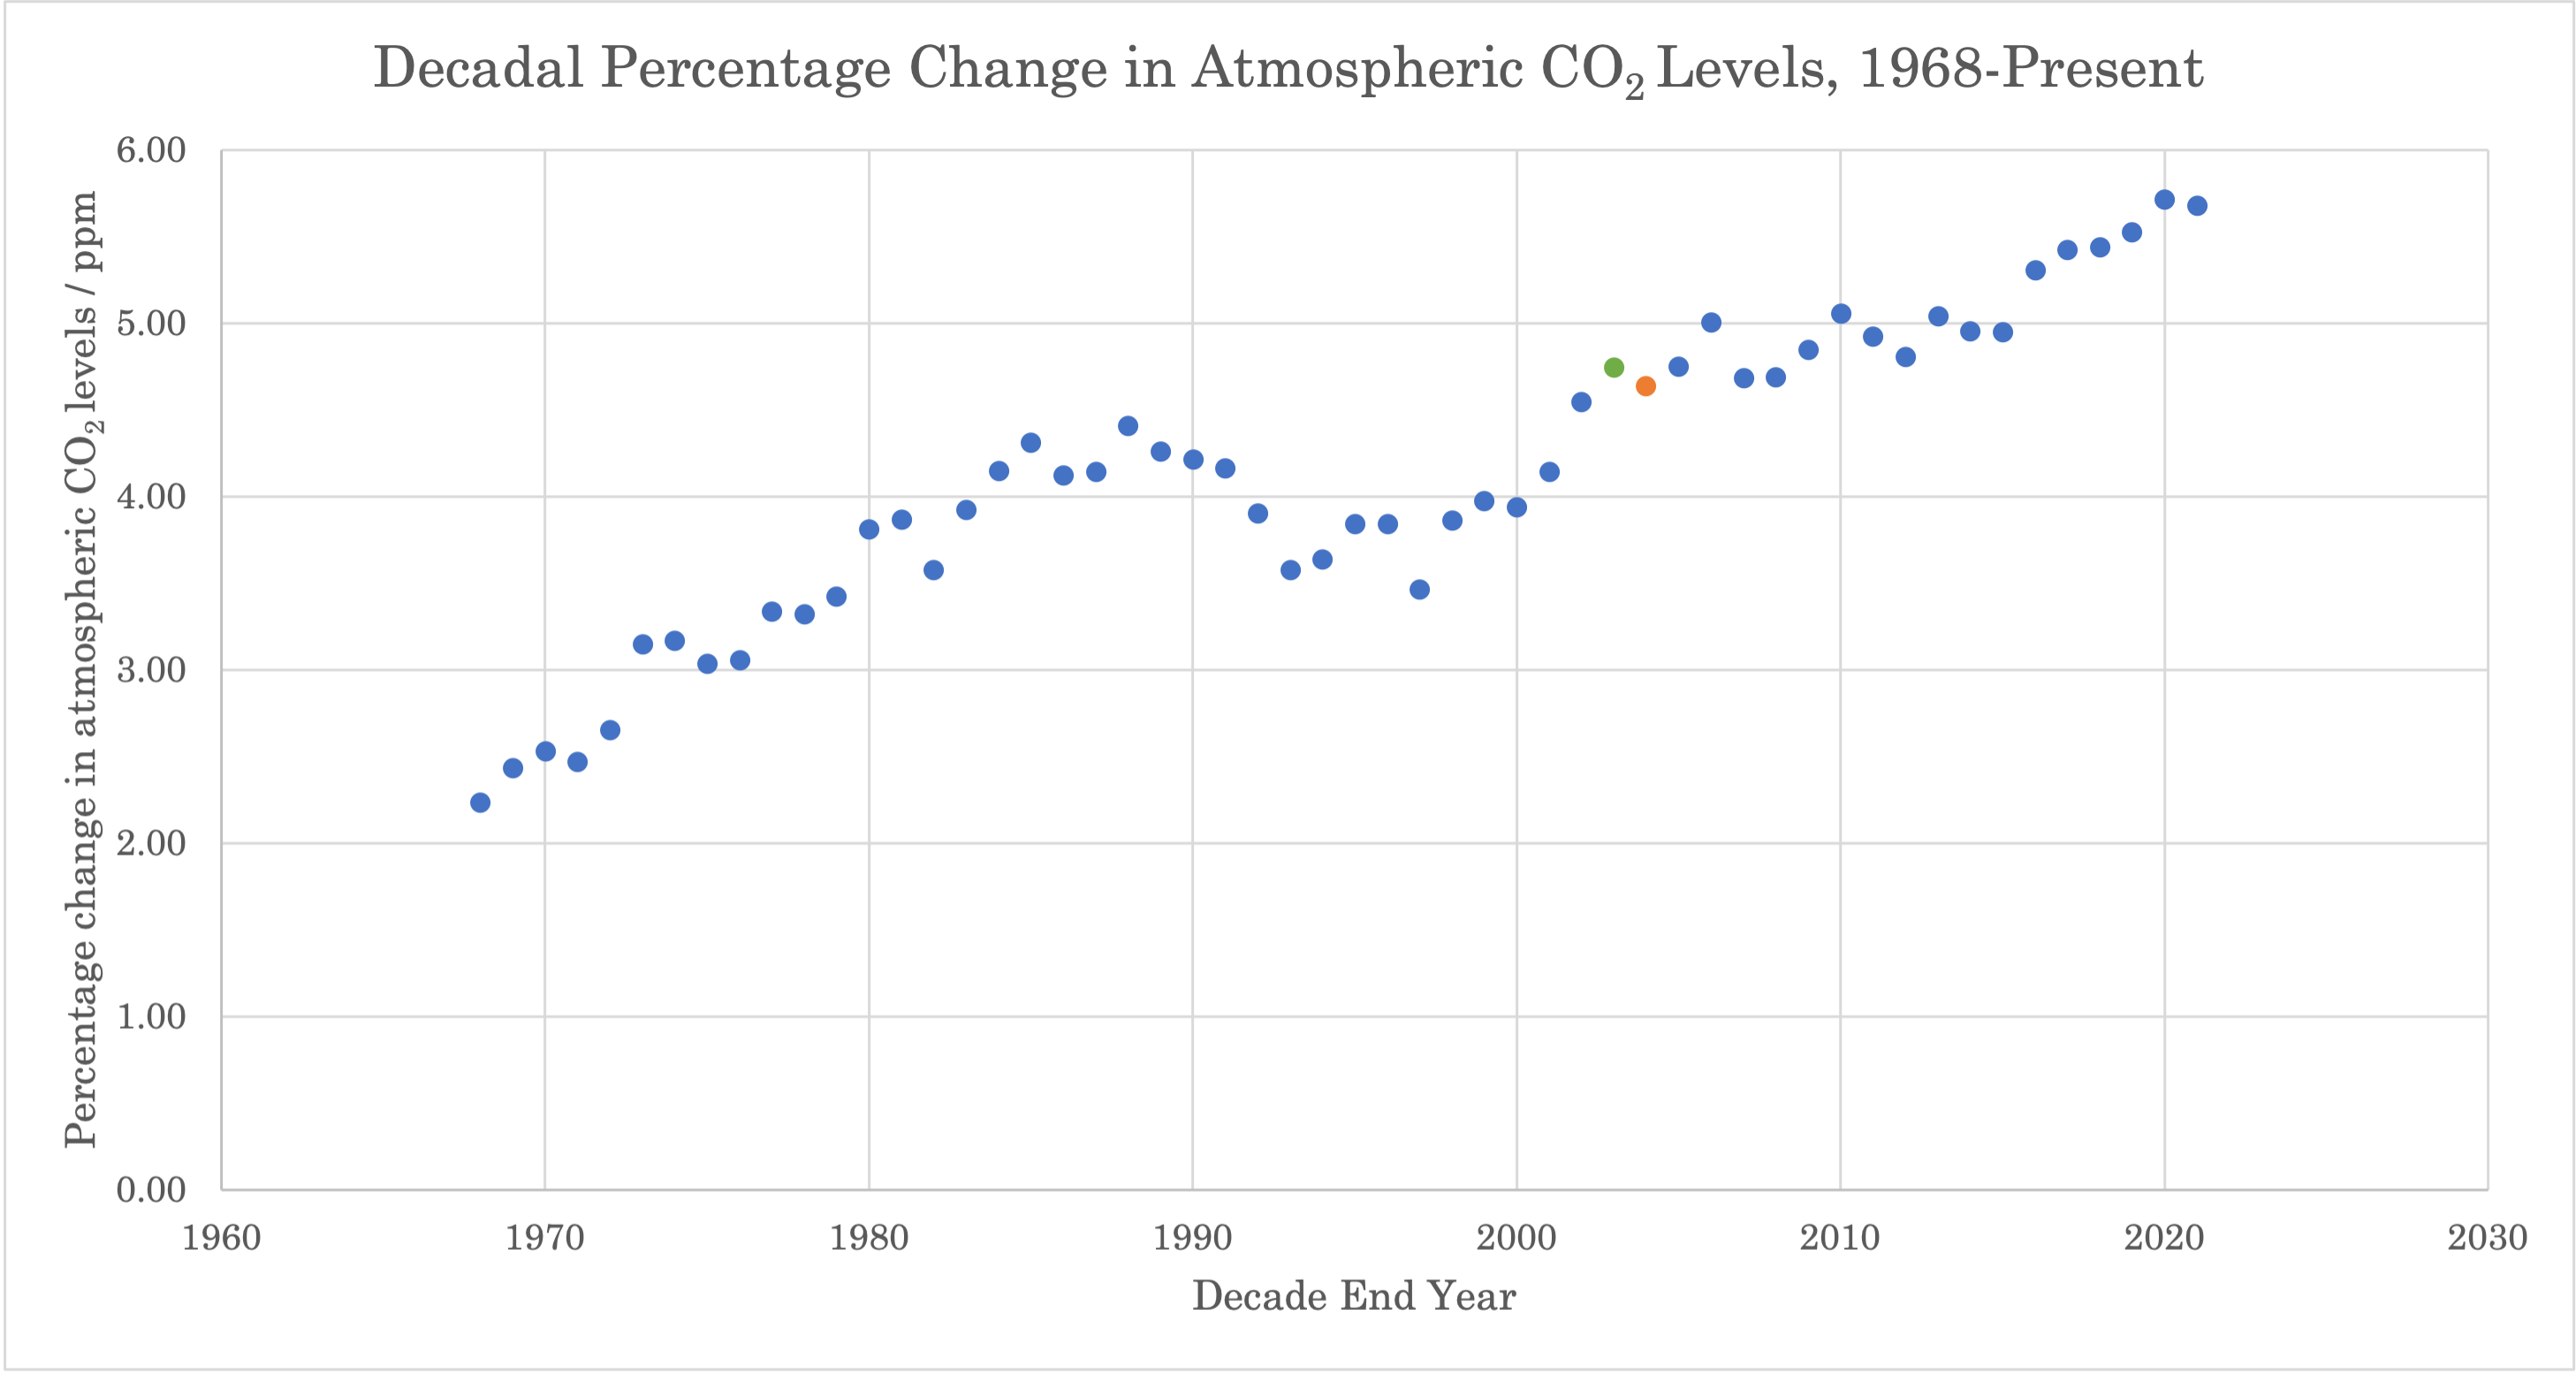
\includegraphics[width=0.6\textwidth]{1a_10y_chg_rel}
        \caption{Moving Decadal Change}
        \label{fig:1a_1}
    \end{wrapfigure}

    As indicated in Figure~\ref{fig:1a_1}, the net percentage increase in atmospheric CO\textsubscript{2} levels over the ten-year period 1994--2004 (4.63\%), while significant, was lower than that of the period1993--20033 (4.74\%). With regard to the available data, the March 2004 increase was therefore only the second-highest recorded over any previous 10-year period.

    \noindent\size{12}{\textbf{Comparing to moving averages}}

    In addition to direct inter-decade comparisons, an analysis of change relative to the average values for each ten-year period was undertaken using the following methodology.

    Using a moving ten-year window, the annual data was divided into 54 overlapping intervals.
    For each interval, the arithmetic average of the annual CO\textsubscript{2} levels was calculated.
    To create a ratio-based indicator, $\propto$, for the extent of change, the following step was further applied:
%
    \begin{equation}
        \propto = \frac{C_f}{\mu}
    \end{equation}
%
    where
    $C_f$ is CO\textsubscript{2} level in the decade end year
    $\mu$ is ten-year arithmetic average CO\textsubscript{2} level.

    The indicator thus provides a convenient and comparable measure for the increase in CO\textsubscript{2} levels at the end of each decade, relative to the ten-year average. A comparison of the-values calculated over the available data yielded the following result, represented visually in Figure~\ref{fig:asdf}, below.
%
    \begin{figure}[h]
        \centering
        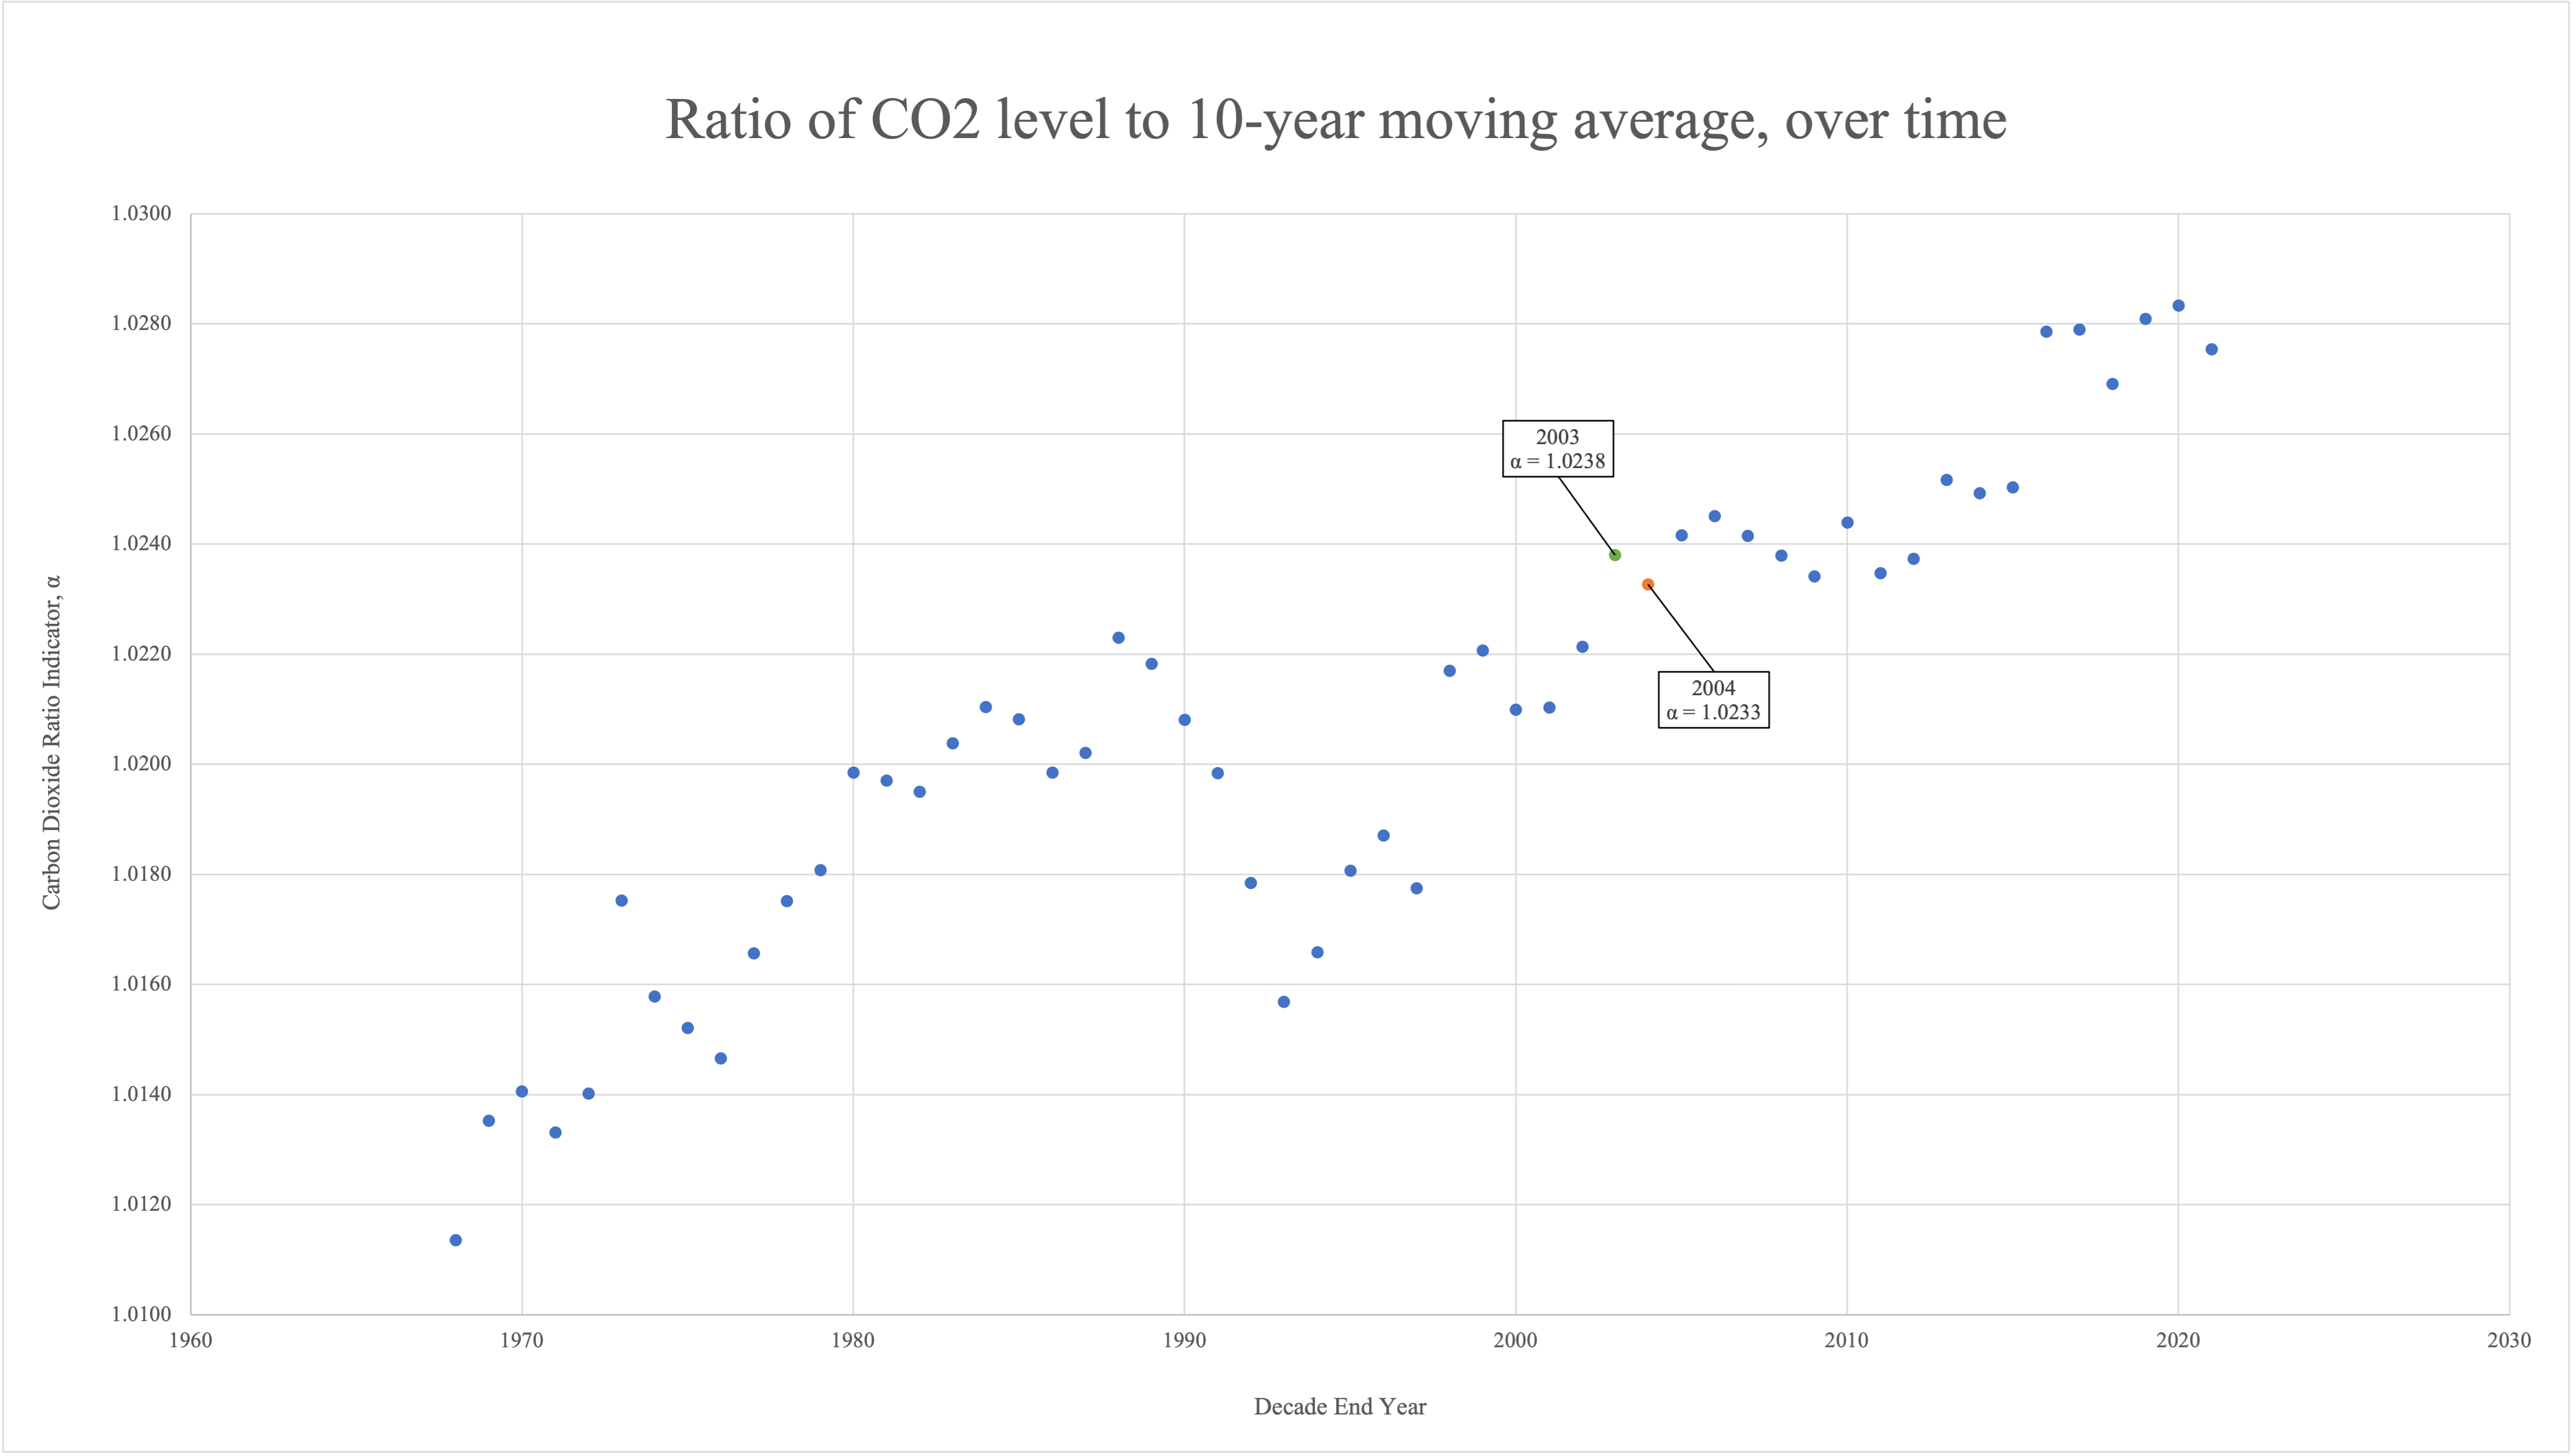
\includegraphics[width=0.8\linewidth]{1a_10y_mv_avg_rel}
        \caption{Moving Decadal Average}
        \label{fig:asdf}
    \end{figure}

    Relative to previous years, the value of $\alpha$ for the decade ending in 2004 (1.0233) was the second-highest calculated, exceeded by that of 2003 (1.0238). This implies that the intra-decade increase for March 2004, in comparison to previous decades, was not the highest.

    A similar procedure was implemented to determine the relative annual increases, using the following formula to calculate a ratio $\beta$:
%
    \begin{equation}
        \beta = \frac{I_f}{\mu_i}
    \end{equation}
%
    where $I_f$ is the final increase, from the second-last to the last year in a given ten-year period; and
    $\mu_i$ is the arithmetic average yearly increase over the ten-year period.

    This yielded a corroborating result, with the $\beta$-value for the decade ending in 2004 (1.217) lower than that of 14 other preceding decade groups.
%
    \begin{figure}[h]
        \centering
        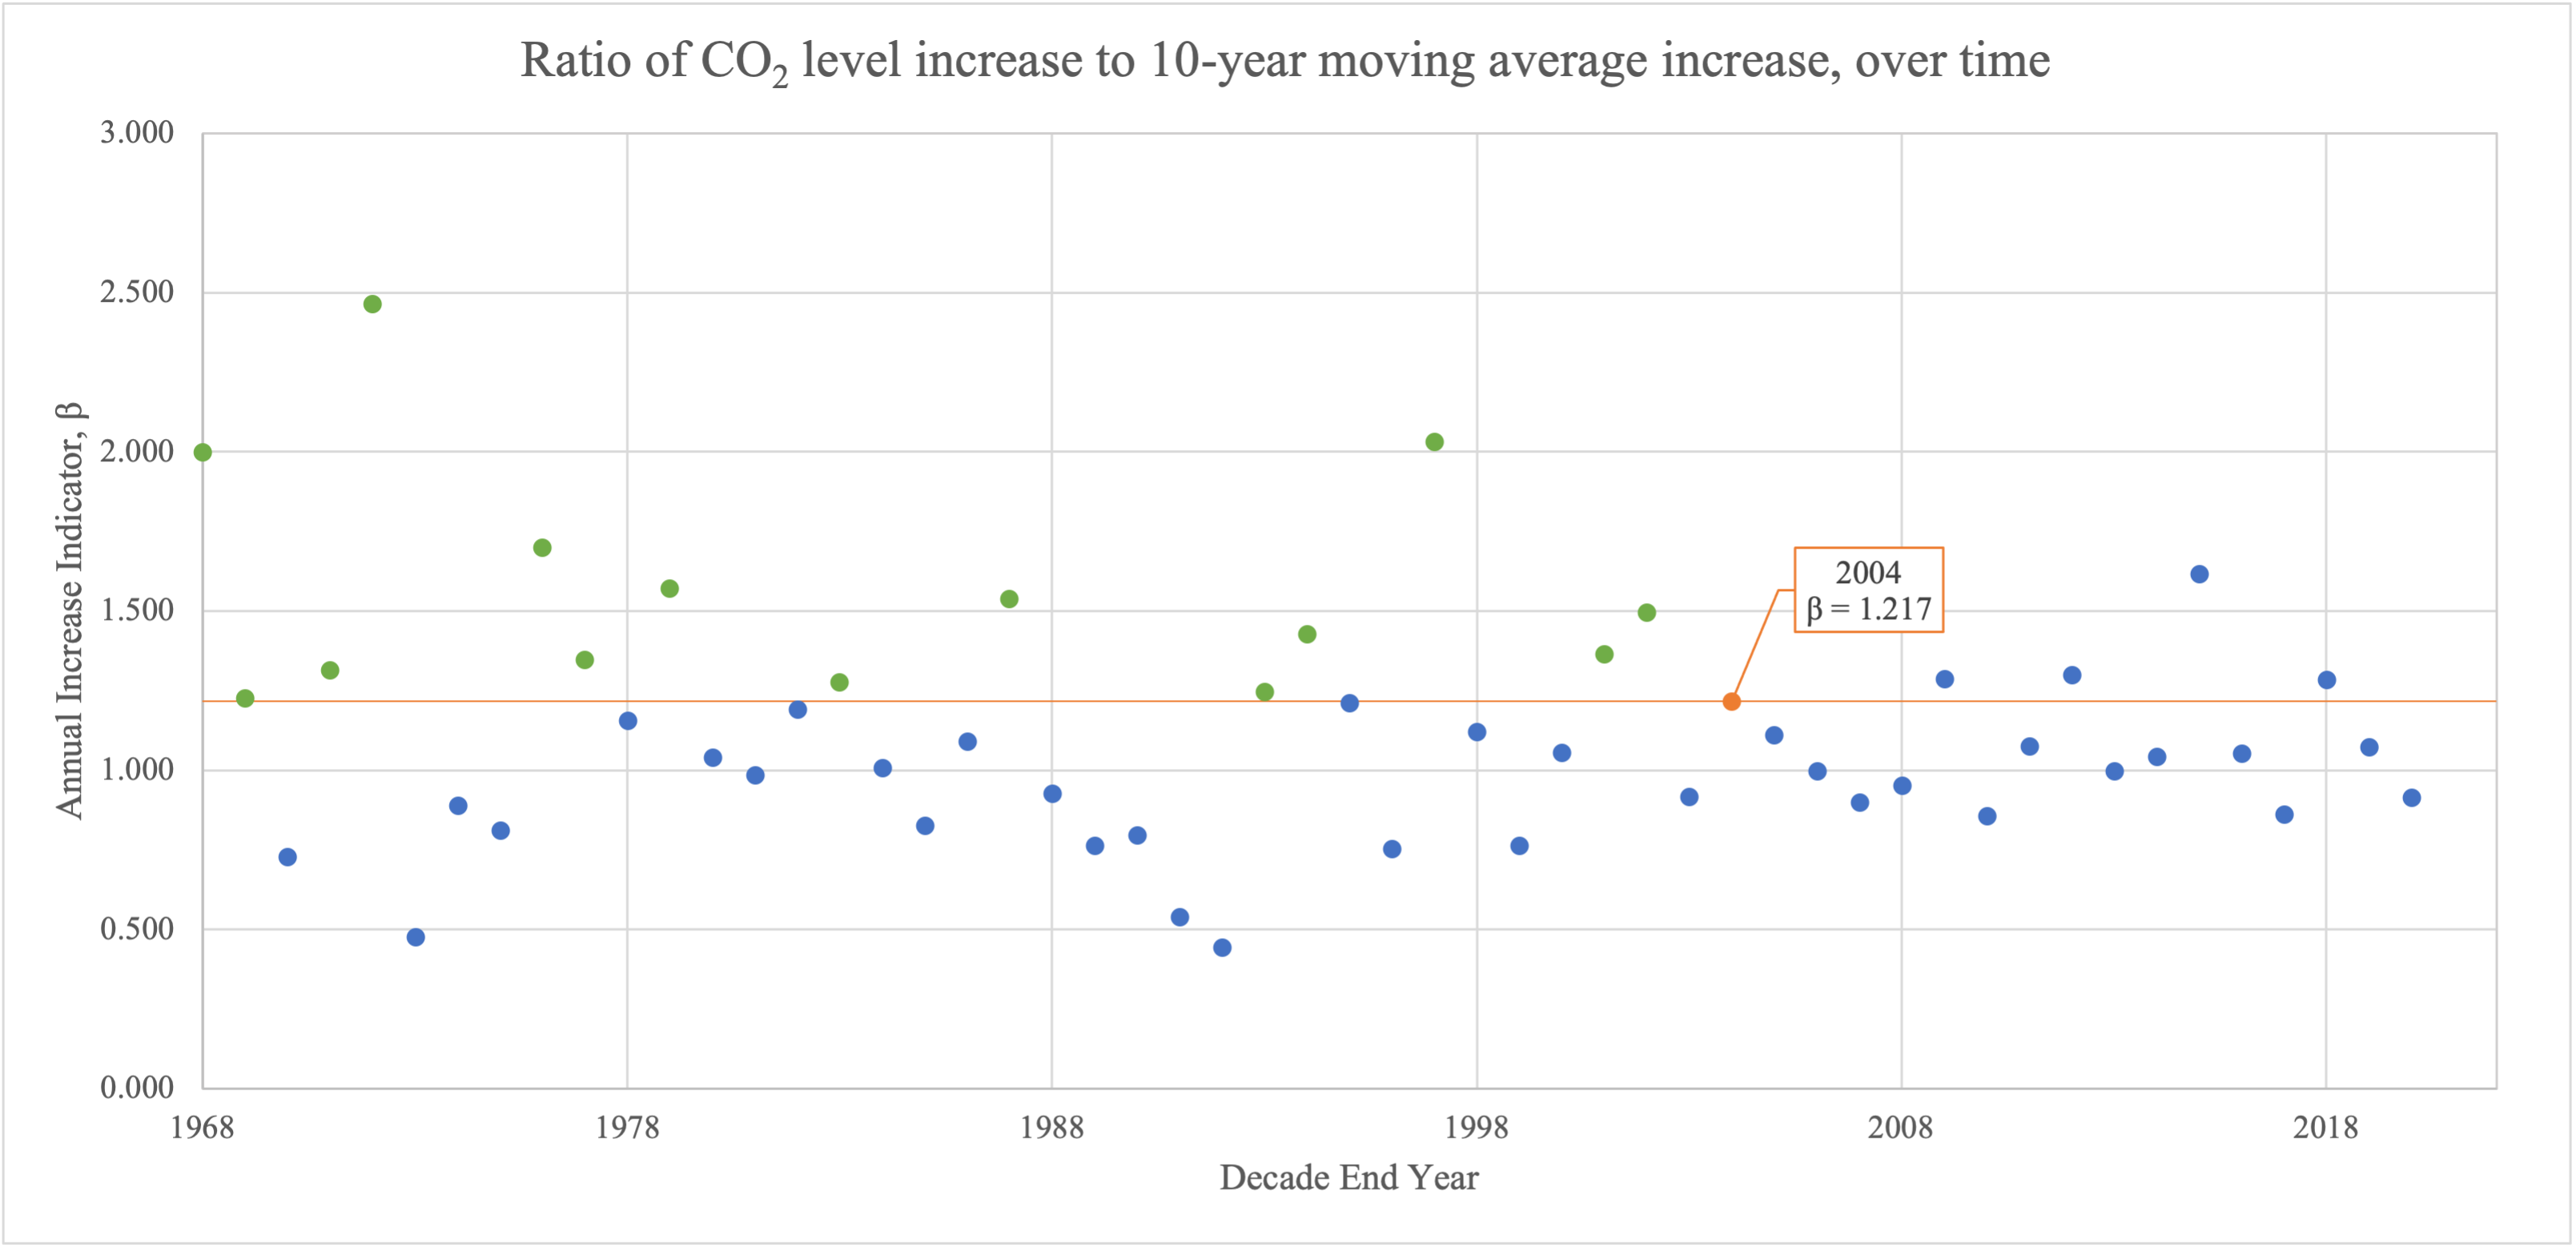
\includegraphics[width=0.8\linewidth]{1a_10y_mv_avg_chg_rel}
        \caption{Moving Decadal Average Change}
        \label{fig:asdfasdf}
    \end{figure}
%

    Therefore, the intra-decade change for 1994--2004 is significantly smaller than that of multiple preceding decades.



    In summary, both approaches yielded an identical conclusion; while the March 2004 increase of CO\textsubscript{2} was among the largest observed until that date, it was not the single largest. In terms of net change and increase from the decadal mean, it was exceeded by the change as of March 2003. Furthermore, its final increase relative to the average annual increase within the ten-year period was significantly smaller than several preceding decade intervals.


    \subsubsection*{OECD: reaching 685ppm by 2050}

   Quoted from the problem statement: ``An Organisation for Economic Co-Operations and Development (OECD) report predicts a CO\textsubscript{2} level of 685ppm by 2050.''.

    Unlike the claim above, this one is straightforward to verify. According to data presented in Table~\ref{tab:co2_685}, no models constructed were close to the year proposed by this claim; even the fastest-growing model, the exponential model, predicted a minimum of 2081 to reach 685ppm.
    All other models provide even further estimates.

    There is a simple explanation for this discrepancy. The OECD never claimed a 686ppm level of \textit{carbon dioxide} by 2050, but rather of \textit{all greenhouse gases}. Naturally, this figure will be higher than CO\textsubscript{2} alone, because CO\textsubscript{2} only accounts for 76\% of all greenhouse gases.


    \section{Temperature - Modelling}

    The model chosen to both forecast future temperature changes and to investigate whether a relationship exists between CO2 emissions and temperatures is a linear regression model. Although it was previously evaluated that Prophet and exponential regression were the most accurate models in forecasting future CO2 emissions, it will not be used for this section. The reason for the exponential model’s success is mainly attributed to the data set’s visibly curved trend, suggesting an exponential or power trend. An exponential relationship was confirmed after practical modelling.

    On the other hand, temperature visually follows a more steadily linear trend; curves and deviations are not as apparent, hence the model was chosen to further investigate and confirm the trend. Additionally, to support this decision, linear regression is a popular and common approach used to model the relationship between an independent and a dependent variable (this case being CO2 emissions and temperature respectively), and hence would be the most optimal model to use for temperature/CO2 analysis.

    \begin{wrapfigure}{r}{0.6\textwidth}
        \centering
        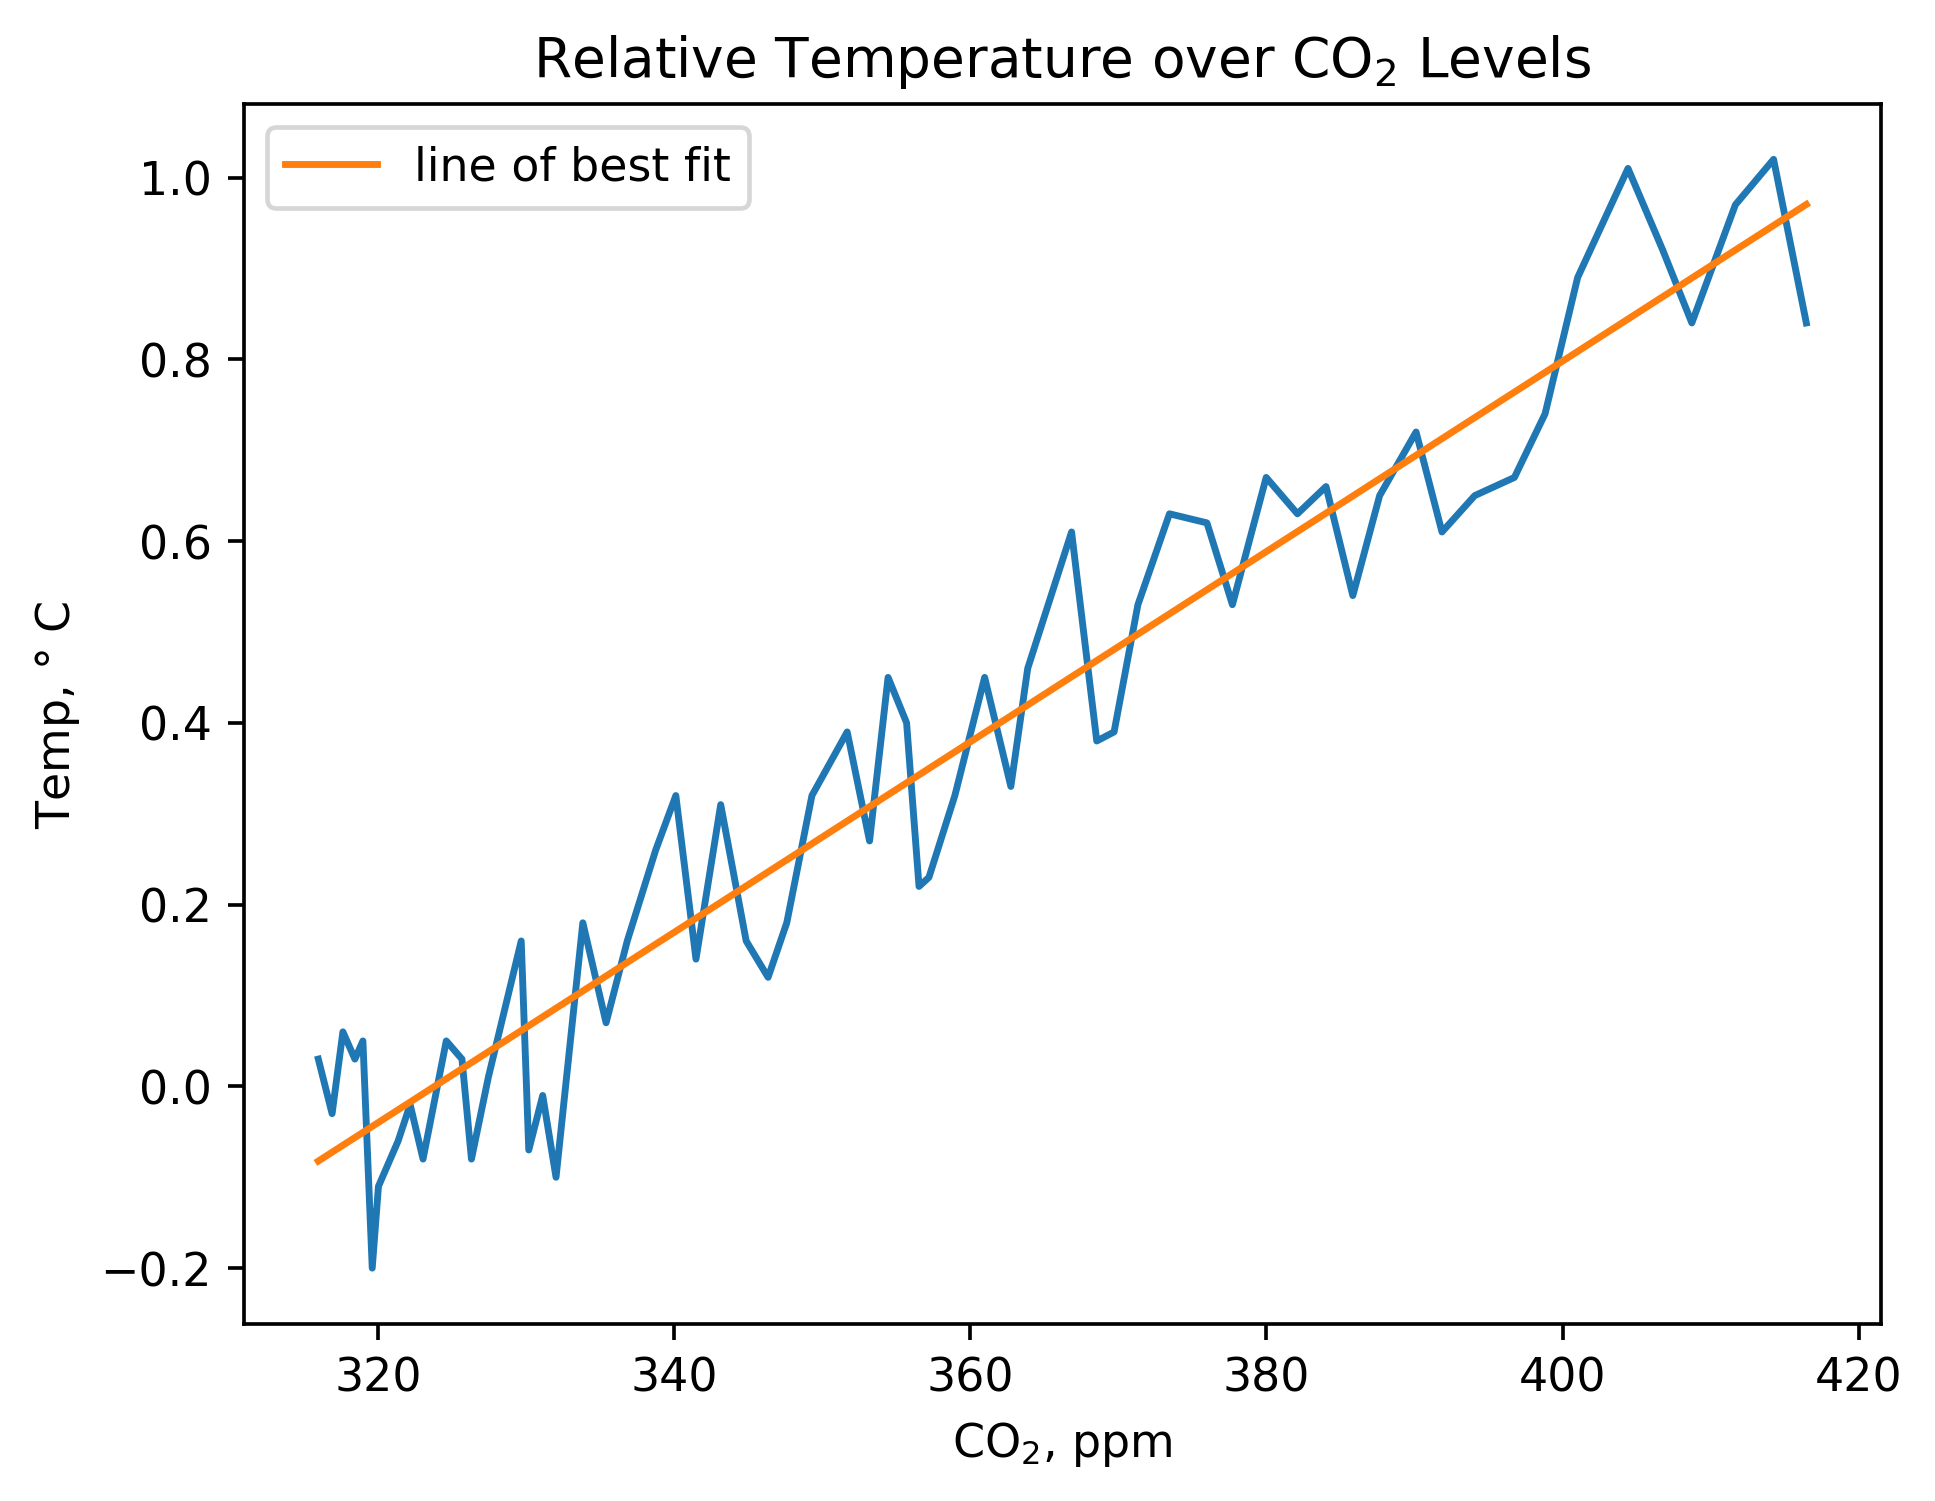
\includegraphics[width=0.6\textwidth]{ct2}
        \caption{Temperature over CO\textsuperscript{2}}
        \label{fig:ct}
    \end{wrapfigure}

    To begin, the values for each variable are plotted onto a graph, and a regression line drawn which can be analysed, allowing other values to be predicted based on existing values. For simple regression, the form of model (trend line) can be defined as.

    The regression line (Figure~\ref{fig:ct}) shows the relationship between the two variables, where PCC is used to measure the correlation strength. The coefficient of determination was determined by squaring the PCC value. R\textsuperscript{2} measures the proportion of variation in the temperatures and CO\textsubscript{2} levels. Covariance was also calculated, and this measures the directional relationship between the x and y variable. The definitions and results for PCC and covariance are denoted in Table~\ref{tab:mm}.



    \section{Temperature - Evaluation}

    \subsection{Accuracy \& Correlation}

    \begin{table}[h]
        \begin{tabular}{|*2{p{.5\textwidth}|}}
            \hline & \\
            \quad ${\displaystyle r={\frac {\sum (x_{i}-{\bar {x}})(y_{i}-{\bar {y}})}{{\sqrt {\sum (x_{i}-{\bar {x}})^{2}}}{\sqrt {\sum (y_{i}-{\bar {y}})^{2}}}}}}$ & ${\displaystyle cov_{x,y}={\frac {\sum (x_{i}-{\bar {x}})(y_{i}-{\bar {y}})}{{N-1}}}}$\\[\baselineskip]
            Where
            \begin{itemize}[nosep]
                \item {r} = Correlation coefficient
                \item ${x_i}$ = Values of the x-variable in a sample
                \item ${\overline x}$ = Mean of the values of the x-variable
                \item ${y_i}$ - Values of the y-variable in a sample
                \item ${\overline y}$ = Mean of the values of the y-variable
            \end{itemize}
            &
            Where
            \begin{itemize}[nosep]
                \item ${cov_{x,y}}$ = Covariance between variable x and y
                \item ${x_i}$ = Data value of x
                \item ${y_i}$ = Data value of y
                \item ${\bar{x}}$ = Mean of x
                \item ${\bar{y}}$ = Mean of y
                \item {N} = Number of data values
            \end{itemize}
            \\
            \hline
        \end{tabular}
        \caption{More Metrics}
        \label{tab:mm}
    \end{table}%
    \begin{table}[H]
        \centering
        \begin{tabular}{ |c|c|c|}
            \hline
            \textbf{PCC} & \textbf{R\textsuperscript{2}} & \textbf{Covariance}\\
            \hline
            0.9599812208926523 & 0.9215639444665472 & 9.20384156682028\\
            \hline
        \end{tabular}
    \end{table}

    The PCC and covariance values obtained indicate a very strong positive correlation between CO\textsubscript{2} emissions and temperature. As for the R\textsuperscript{2} value, it indicates that 92\% of the variability observed in temperature can be explained by CO\textsubscript{2} emissions. Hence, the conclusion can be formed that there exists a strong positive relationship between CO\textsubscript{2} emissions and temperature.

    As the existence of the relationship has been confirmed and justified, the regression line can be used to extrapolate future data. A temperature over time model was constructed and extended 30 years in the future to forecast future temperatures. The results are plotted in Figure~\ref{fig:temp_pred}; the highlighted region indicates the margin of error and the black points indicate the actual observed values.

    \begin{figure}[h]
        \centering
        \begin{minipage}{0.45\linewidth}
            \centering
            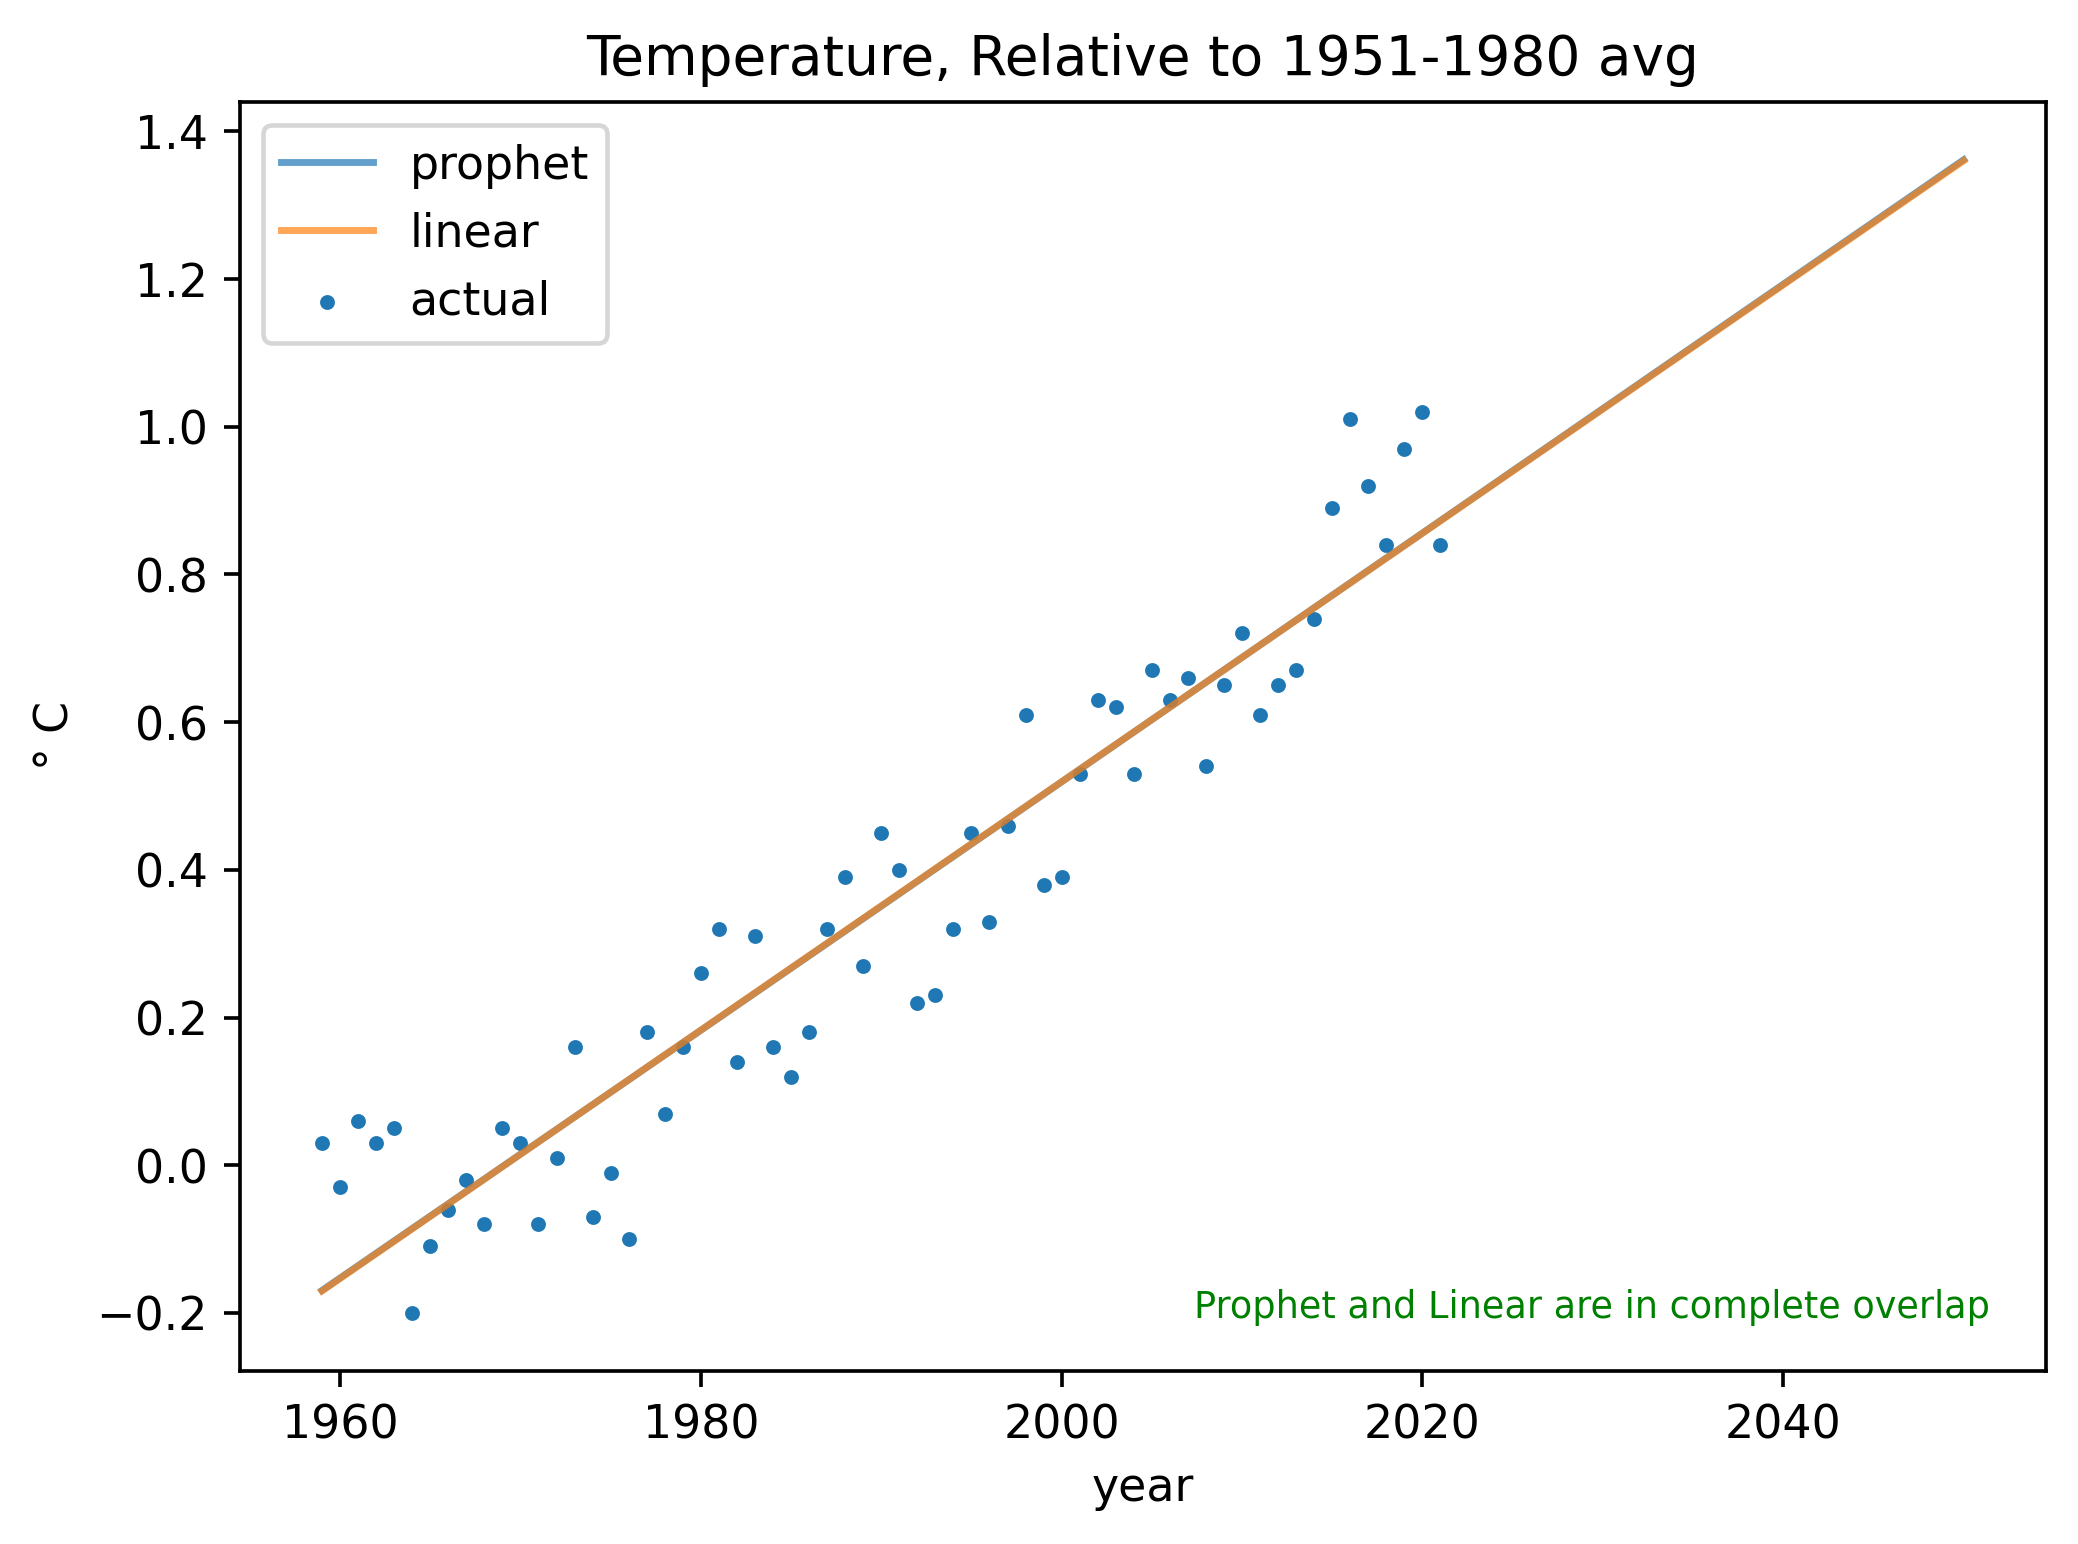
\includegraphics[width=\textwidth]{temp_pred}
        \end{minipage}%
        \begin{minipage}{0.55\linewidth}
            \centering
            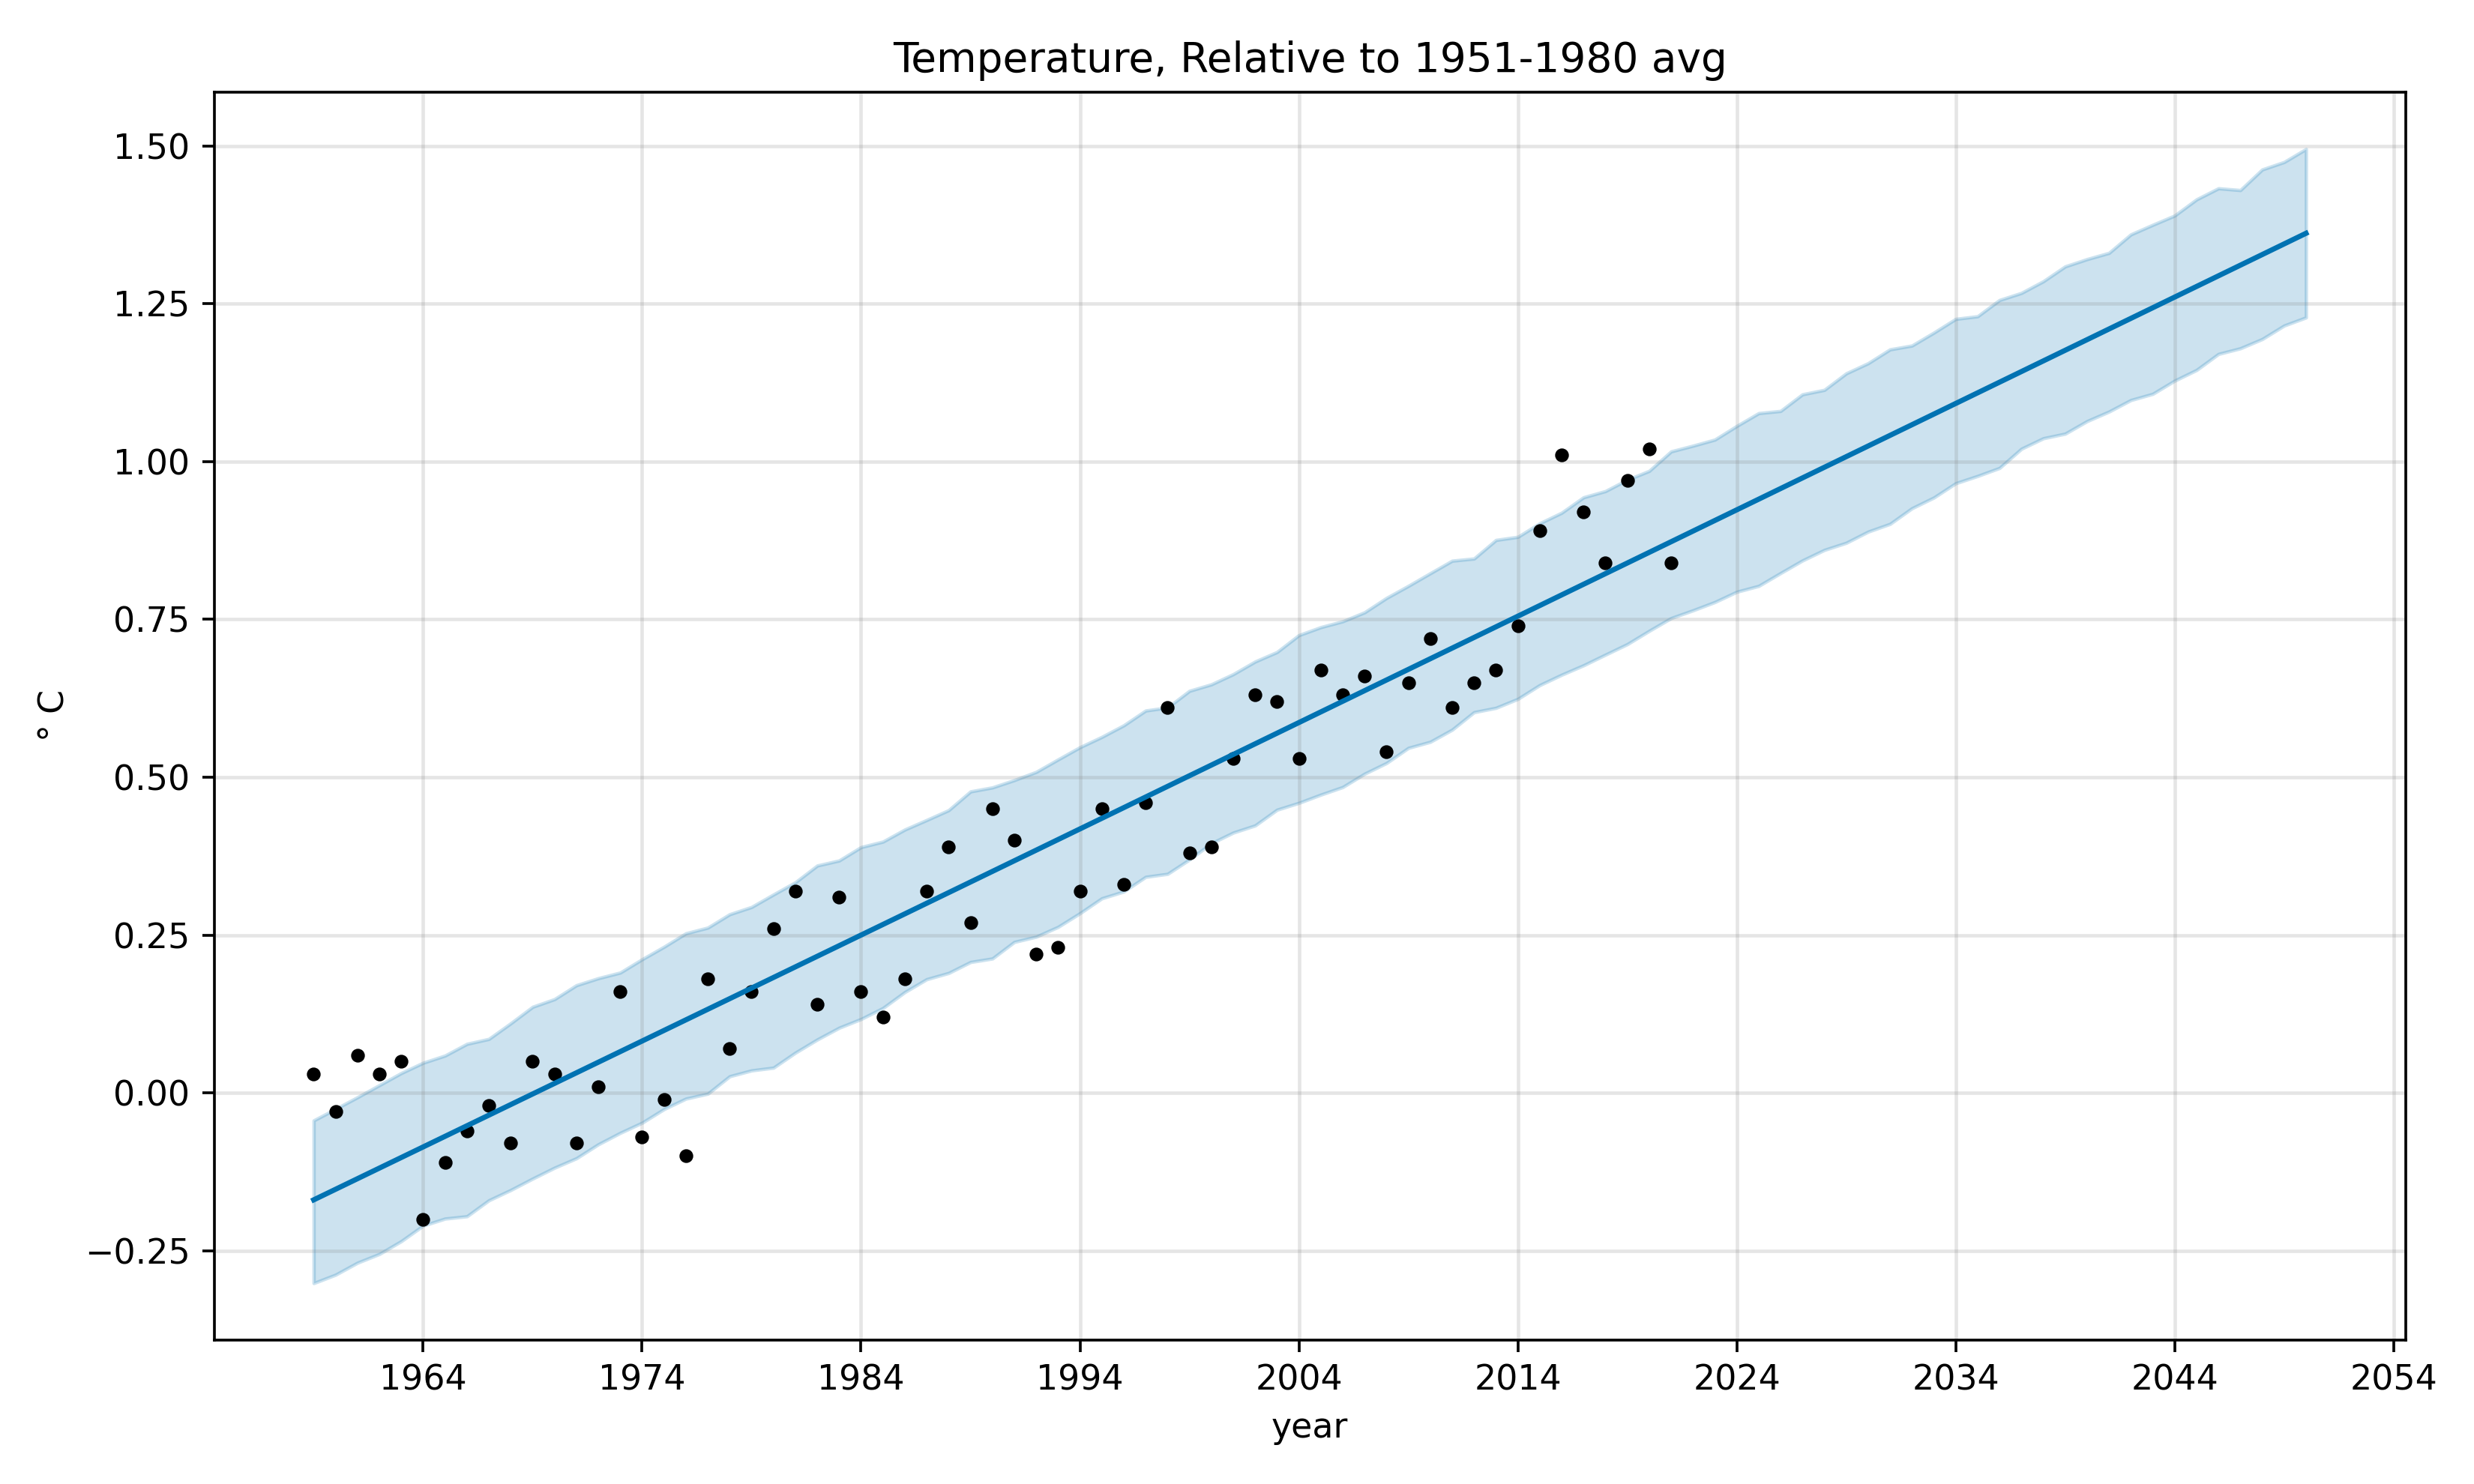
\includegraphics[width=\textwidth]{temp_prophet}
        \end{minipage}
        \caption{Linear Temperature Predictions}
        \label{fig:temp_pred}
    \end{figure}


    As can be observed, the regression line’s margin of error extends to cover the vast majority of known value points. Additionally, what can be remarked is that the Prophet model was applied to the data to produce a completely identical trend-line to that of linear regression. It was previously argued in the introduction that Prophet and exponential modelling would not be used as visually, linear regression indicated the best fit. However, this argument applied mainly to the CO2 and temperature relationship. Prophet is capable of producing a more nuanced model that accounts for varying parameters; hence, the fact that its application yields an identical result to that of linear regression supports the initial argument that the best model option is linear regression.


    \subsection{Predictive Ability}

    \noindent\textbf{Temperature over CO\textsubscript{2} Model}

    The linear model relating CO2 level to temperature is accurate and reliable when performing interpolation, since it fits existing data points with a very high coefficient of determination of 0.924. However, in order to predict future temperatures based on future CO2 levels, extrapolation must be performed on the CO2 model. By nature, extrapolation is less accurate than interpolation. This implies a lower forecast reliability of the model, as the assumption is made that the relationships remain unchanged.

    Regardless, current data exhibits a very strong linear relationship between CO2 and temperature, as shown by a PCC of 0.961. Prophet, which is able to fit to complex trends and perform highly accurate interpolation, simply produced a perfectly linear model. This supports the conclusion that the best model is a linear relationship, and that the relationship shows no sign of changing in the future.

    The three linear regression models - CO2-time, CO2-temperature, and temperature-time - are linked together by the fact that the relationship between CO2 and temperature exhibits a  strong statistical correlation. It is scientifically proven that CO2 and temperature have a cause-and-effect relationship, due to the greenhouse effect, where CO2 has a warming effect. This provides a link between the three models, where all three variables correlate strongly. This multi-variable correlation supports the accuracy of each individual model. On the contrary, if there is an unforeseen change in one of the relationships, all models will be incorrect.

    Another approach to verify the accuracy and reliability of the models was to compare the predictions with external sources (existing literature). This can help us analyse the reliability of the forecast.

    Values of CO2 concentration and Temperature Rise from secondary sources projected for 2100

    \begin{center}
        \begin{tabular}{ |c|c|}
            \hline
            \textbf{CO\textsubscript{2} (ppm)} & \textbf{Temperature Rise (C)} \\
            \hline
            701 & 2.2 \\
            \hline
        \end{tabular}
    \end{center}

    \begin{center}
        \begin{tabular}{ |c|c|c|}
            \hline
            Data from: & \textbf{CO\textsubscript{2} (ppm)} & \textbf{Temperature Rise (C)} \\
            \hline
            Confirmed Proposals (2011) & 900 & 4.0 \\
            \hline
            INDCs Strict (2015) & 670 & 3.5 \\ \hline
            2C Pathway (2015) & 475 & 2.0 \\ \hline
            1.8C Pathway (2015) & 450 & 1.8 \\ \hline
            1.5C Pathway (2015) & 425 & 1.5 \\ \hline
            2014 `Actuals' & 397 & 0.9 \\ \hline
            \textbf{Mean} & 536.16567 & 2.283333 \\ \hline
            \textbf{Standard Deviation} & 161.49974 & 1.206681 \\ \hline
        \end{tabular}
    \end{center}


    \noindent\textbf{Temperature over Time Model}

    As linear regression’s accurate predictive ability has been confirmed, the equation line can then be used to obtain the years at which a temperature change of 1.25C, 1.5C and 2C will occur, compared to the base period. External predicted year values were obtained from carbonbrief.org as comparison. The results are presented in the table below:

    \begin{table}[h]
        \centering
        \begin{tabular}{ |c|c|c|c|}
            \hline
            & \textbf{1.25C} & \textbf{1.5C} & \textbf{2C}         \\
            \hline
            \textbf{Linear Regression} & 2043           & 2058          & 2088                \\
            \hline
            \textbf{External}          & N/A            & 2026--2042    & 2043--2052 \\ \hline
        \end{tabular}
    \end{table}

    The year values obtained are generally higher in comparison to the external values, which is possibly due to the spike in temperature from 2018--2021. The spike may have caused the gradient of the regression line to increase to accommodate for the sudden temperature increases, which in turn led to higher values.



    \section{References}

%    \printbibliography

\end{document}
